\documentclass[12pt,a4paper]{article}
\usepackage[utf8]{inputenc}
\usepackage{amsmath}
\usepackage{amsfonts}
\usepackage{amssymb}
\usepackage{graphicx}
\graphicspath{ {./img/} }
\usepackage{hyperref}
\usepackage{array}
\usepackage[table]{xcolor}
\usepackage{xcolor,colortbl}
\usepackage{multirow}
\usepackage[a4paper, total={6in, 8in}]{geometry}

\usepackage{titlesec}

\setcounter{secnumdepth}{4}

\titleformat{\paragraph}
{\normalfont\normalsize\bfseries}{\theparagraph}{1em}{}
\titlespacing*{\paragraph}
{0pt}{3.25ex plus 1ex minus .2ex}{1.5ex plus .2ex}

\author{Natale Guadagno, Paolo Patrone}
\title{Requisites Analysis Document - TecStore}
\renewcommand{\contentsname}{Contenuti}

\usepackage{hyperref}
\hypersetup{
    colorlinks,
        citecolor=blue,
    filecolor=blue,
    linkcolor=blue,
    urlcolor=blue,
    linktocpage
}

\begin{document}

\maketitle
\newpage
\tableofcontents
\newpage
\newgeometry{top=0.5in,bottom=0.5in,right=0.5in,left=0.5in}
\section*{Partecipanti}
\begin{center}
\begin{tabular} {|c|c|}
\hline
\textbf{Nome} & \textbf{Matricola} \\
\hline
Guadagno Natale & 0512106546 \\
Patrone Paolo & 0512106153 \\
\hline
\end{tabular}
\end{center}


\section*{Revision History}
\begin{center}
\begin{tabular} {|c|c|c|}
\hline
\textbf{Data} & \textbf{Versione} & \textbf{Descrizione} \\
01/12/2021 & 0.1 & Prima stesura \\
02/12/2021 & 0.2 & Requisiti funzionali \\
\hline

\hline
\end{tabular}
\end{center}

\newpage

\section{Introduzione}

\subsection{Scopo del sistema}
Il sistema si pone l'obiettivo di facilitare le operazioni di gestione e controllo di operazioni di compravendita e di operazioni gestionali che non sono a carico dell'utenza, come la gestione del personale e dell'inventario. Sono previste viste e interfacce distinte per le varie operazioni per semplificare l'utilizzo ed evitare confusione.

\subsection{Ambito del sistema}
TecStore è una piattaforma web che permette ad utenti di comprare e vendere materiale tecnologico, che può essere messo in vendita da altri utenti o dalla piattaforma stessa. Trattandosi di un negozio piccolo, il catalogo è relativamente limitato, ma si punta a creare utenza attraverso prezzi vantaggiosi e un servizio clienti di qualità.
L'utenza della piattaforma si divide in:
\begin{itemize}
\item Clienti, che, una volta registrati ed autenticati, possono acquistare articoli
\item Venditori, che mettono articoli in vendita
\item Centralinisti, che gestiscono i \emph{ticket}
\item Magazzinieri, che gestiscono le spedizioni degli articoli
\item Amministratori catalogo, che gestiscono gli articoli messi in vendita dalla piattaforma
\item Amministratori personale, che gestiscono la presenza nel sistema dei dipendenti
\end{itemize}

\subsection{Obiettivi del progetto}
 TODO

\subsection{Definizioni, acronimi ed abbreviazioni}
 TODO

\section{Sistema proposto}
 TODO
 
\subsection{Identificazione attori}
 TODO
 
\subsection{Requisiti funzionali}
\begin{center}
\begin{tabular}{|c|l|c|}
\hline
\rowcolor[gray]{0.8}
\textbf{Funzionalità} & \textbf{Requisito} & \textbf{Priorità} \\
\hline
\multirow{8}{*}{Clienti} & 3.1.1 Registrazione & Alta \\
& 3.1.2 Autenticazione & Alta \\
& 3.1.3 Acquisto & Alta \\
& 3.1.4 Annullamento & Media \\
& 3.1.5 Vendita & Media \\
& 3.1.6 Assistenza & Alta \\
& 3.1.7 ModificaProfilo & Bassa \\
& 3.1.8 RecuperoPassword & Media \\
\hline
\multirow{5}{*}{Gestione} & 3.2.1 GestioneOrdini & Alta \\
& 3.2.2 GestioneTicket & Alta \\
& 3.2.3 ControlloArticoli & Alta \\
& 3.2.4 GestionePersonale & Alta \\
& 3.2.5 GestioneCatalogo & Alta \\

\hline
\end{tabular}
\end{center}

\subsubsection{Clienti}
Questa funzionalità racchiude tutte le operazioni fornite agli utenti.

\paragraph*{Registrazione}
\begin{center}
\begin{tabular}{|c|c|}
\rowcolor[gray]{0.8}
\hline
\textbf{Attore} & \textbf{Funzionalità} \\
Cliente non registrato & Permette di registrarsi. \\
\hline
\end{tabular}
\end{center}

\paragraph*{Autenticazione}
\begin{center}
\begin{tabular}{|c|c|}
\rowcolor[gray]{0.8}
\hline
\textbf{Attore} & \textbf{Funzionalità} \\
Cliente registrato & Permette di autenticarsi. \\
\hline
\end{tabular}
\end{center}

\paragraph*{Acquisto}
\begin{center}
\begin{tabular}{|c|c|}
\rowcolor[gray]{0.8}
\hline
\textbf{Attore} & \textbf{Funzionalità} \\
Cliente registrato & Permette di acquistare un articolo. \\
\hline
\end{tabular}
\end{center}

\paragraph*{Annullamento}
\begin{center}
\begin{tabular}{|c|c|}
\rowcolor[gray]{0.8}
\hline
\textbf{Attore} & \textbf{Funzionalità} \\
Cliente registrato & Permette di annullare un ordine. \\
\hline
\end{tabular}
\end{center}

\paragraph*{Vendita}
\begin{center}
\begin{tabular}{|c|c|}
\rowcolor[gray]{0.8}
\hline
\textbf{Attore} & \textbf{Funzionalità} \\
Cliente registrato & Permette di vendere un articolo. \\
\hline
\end{tabular}
\end{center}

\paragraph*{Assistenza}
\begin{center}
\begin{tabular}{|c|c|}
\rowcolor[gray]{0.8}
\hline
\textbf{Attore} & \textbf{Funzionalità} \\
Cliente registrato & Permette di richiedere assistenza. \\
\hline
\end{tabular}
\end{center}

\paragraph*{ModificaProfilo}
\begin{center}
\begin{tabular}{|c|c|}
\rowcolor[gray]{0.8}
\hline
\textbf{Attore} & \textbf{Funzionalità} \\
Cliente registrato & Permette di modificare informazioni del profilo come password, carta di credito e indirizzo. \\
\hline
\end{tabular}
\end{center}

\paragraph*{RecuperoPassword}
\begin{center}
\begin{tabular}{|c|c|}
\rowcolor[gray]{0.8}
\hline
\textbf{Attore} & \textbf{Funzionalità} \\
Cliente registrato & Permette di modificare la password se la si è dimenticata. \\
\hline
\end{tabular}
\end{center}

\subsubsection{Gestione}
Questa funzionalità racchiude tutte le operazioni fornite al personale per la gestione della piattaforma.

\paragraph*{GestioneOrdini}
\begin{center}
\begin{tabular}{|c|c|}
\rowcolor[gray]{0.8}
\hline
\textbf{Attore} & \textbf{Funzionalità} \\
Magazziniere & Permette di confermare la spedizione di un ordine o di annullarlo. \\
\hline
\end{tabular}
\end{center}

\paragraph*{GestioneTicket}
\begin{center}
\begin{tabular}{|c|c|}
\rowcolor[gray]{0.8}
\hline
\textbf{Attore} & \textbf{Funzionalità} \\
Centralinista & Permette di interagire con gli utenti per risolvere un problema. \\
\hline
\end{tabular}
\end{center}

\paragraph*{ControlloArticoli}
\begin{center}
\begin{tabular}{|c|c|}
\rowcolor[gray]{0.8}
\hline
\textbf{Attore} & \textbf{Funzionalità} \\
Centralinista & Permette di filtrare quali articoli messi in vendita vengono accettati. \\
\hline
\end{tabular}
\end{center}

\paragraph*{GestionePersonale}
\begin{center}
\begin{tabular}{|c|c|}
\rowcolor[gray]{0.8}
\hline
\textbf{Attore} & \textbf{Funzionalità} \\
Amministratore personale & Permette di aggiungere, rimuovere e modificare account per i dipendenti. \\
\hline
\end{tabular}
\end{center}

\paragraph*{GestioneCatalogo}
\begin{center}
\begin{tabular}{|c|c|}
\rowcolor[gray]{0.8}
\hline
\textbf{Attore} & \textbf{Funzionalità} \\
Amministratore catalogo & Permette di aggiungere, rimuovere e modificare articoli venduti da TecStore. \\
\hline
\end{tabular}
\end{center}

\newpage

\subsection{Requisiti non funzionali}
\subsubsection{Sicurezza e privacy}
Il sistema deve prevedere tutte le pratiche di sicurezza fondamentali, come l'utilizzo di SSL per la trasmissione dei dati, l'utilizzo di \textit{hashing} e \textit{salt} per le password memorizzate nel database, tutti i dati delle carte di credito e anagrafiche devono essere cifrati prima di essere inseriti nel database utilizzando una cifratura robusta con una chiave che non deve essere esposta pubblicamente per nessun motivo. \\
In accordo con il Regolamento UE 2016/679, anche noto come General Data Protection Regulation, ``GDPR", all'utente sarà descritto l'utilizzo che si farà dei dati raccolti durante il suo uso della piattaforma e sarà possibile la cancellazione totale di tutti i dati pertinenti, meno i dati necessari al mantenimento di un inventario accurato. \\
In caso di tentativo di accesso a schermate riservate da parte di un utente consumatore o viceversa, ovvero un utente del personale che cerca di accedere al catalogo, deve essere previsto un avviso e un \textit{redirect} ad una pagina correttamente accessibile da quel tipo di utente.

\subsection{Affidabilità}
Il sistema deve garantire un \emph{uptime} di almeno il 99.9\%, ovvero un \textit{downtime} annualizzato di meno di 9 ore. Ciò è cruciale per far sì che l'utenza non venga scoraggiata dall'utilizzo di TecStore come negozio primario, creando perdite potenziali molto alte. \footnote{https://www.the20.com/blog/the-cost-of-it-downtime/}

\subsection{Performance}
Il sistema deve prevedere la possibilità di utilizzo di sistemi di \textit{load balancing} per distribuire il carico di utenza in caso di picchi improvvisi tra più server, in modo da garantire l'uso della piattaforma al maggior numero di clienti possibile.

\subsection{Manutenibilità}
Il sistema sarà progettato secondo principi di sviluppo che ne garantiranno la semplicità di aggiornamento, ampliamento e modifica.
Sarà utilizzata un'architettura Three-Tier per separare la gestione dei dati, il programma server e l'interfaccia utente.

\subsection{Implementazione}
Sarà utilizzata la tecnologia JSP con servlet su server Tomcat per la presentazione delle pagine web all'utente , un database MariaDB per la memorizzazione dei dati e ogni utente utilizzerà un comune browser web per accedere al sistema.

\newpage
\subsection{Scenari}
\subsubsection{Un utente non registrato vuole acquistare un articolo}
\textbf{Attore:} Luca Garibaldi, utente non registrato e Massimo Boni, magazziniere \\
\noindent
\textbf{Flusso di eventi:}
\begin{enumerate}
\item Luca ha deciso di effettuare un upgrade al suo computer.

\item Non convinto dai prezzi dei principali venditori, decide di cercare un negozio alternativo e si imbatte in TecStore.

\item Cercando tra le CPU compatibili con la sua scheda madre, si imbatte nella CPU "Intel i5 10400f" a un prezzo scontato rispetto alla concorrenza e decide quindi di effettuare l'acquisto.

\item Aggiunge il componente al carrello. \\

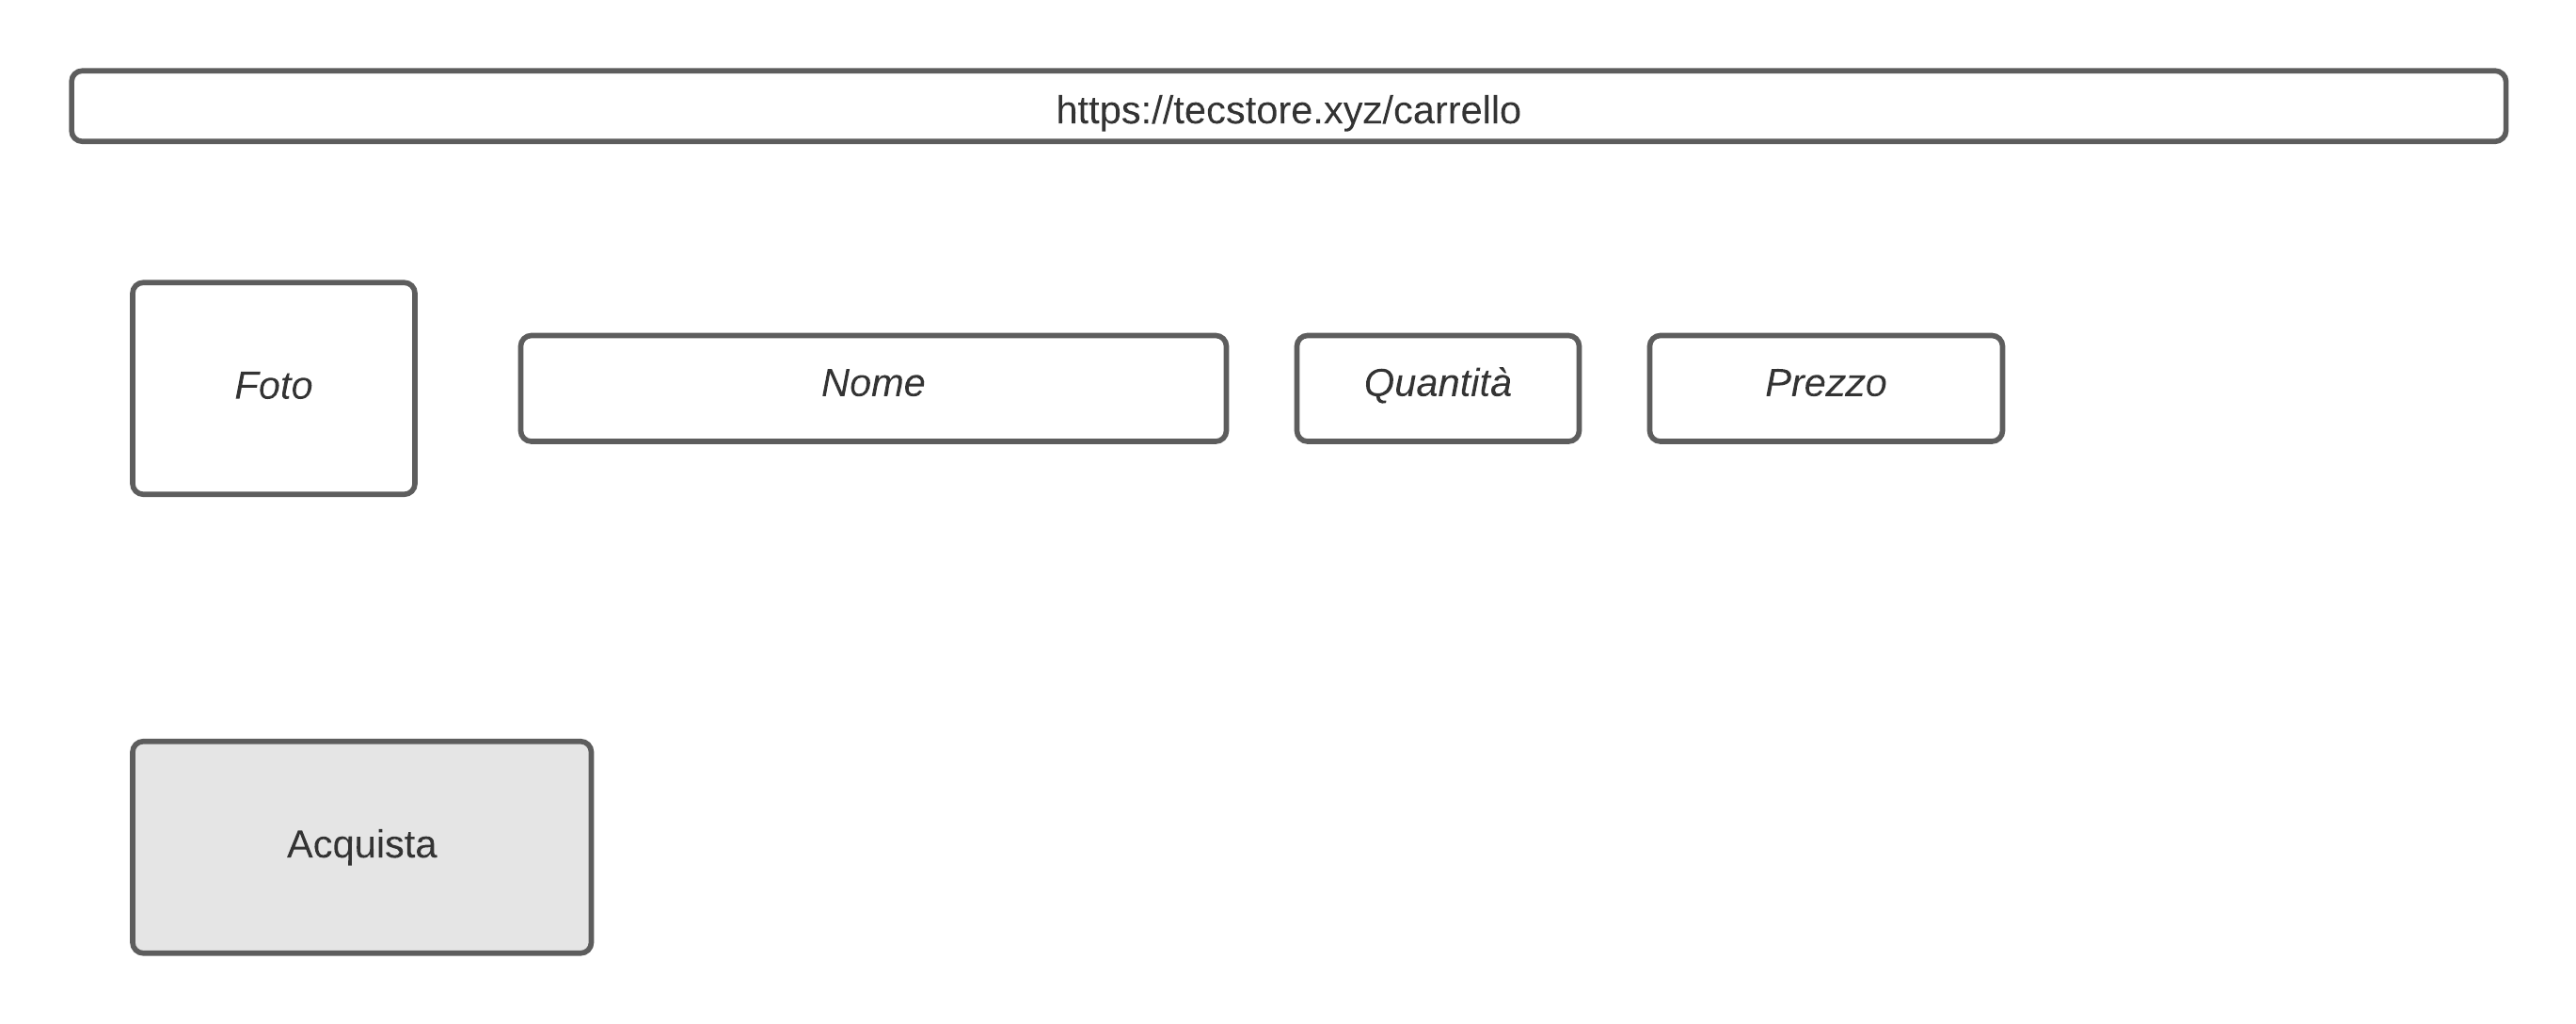
\includegraphics[height=150px]{Mockup/carrello}

\item Fa click sul tasto per effettuare l'ordine e gli viene chiesto di effettuare il login. Dato che non è ancora utente, fa click sul tasto "Registrazione".

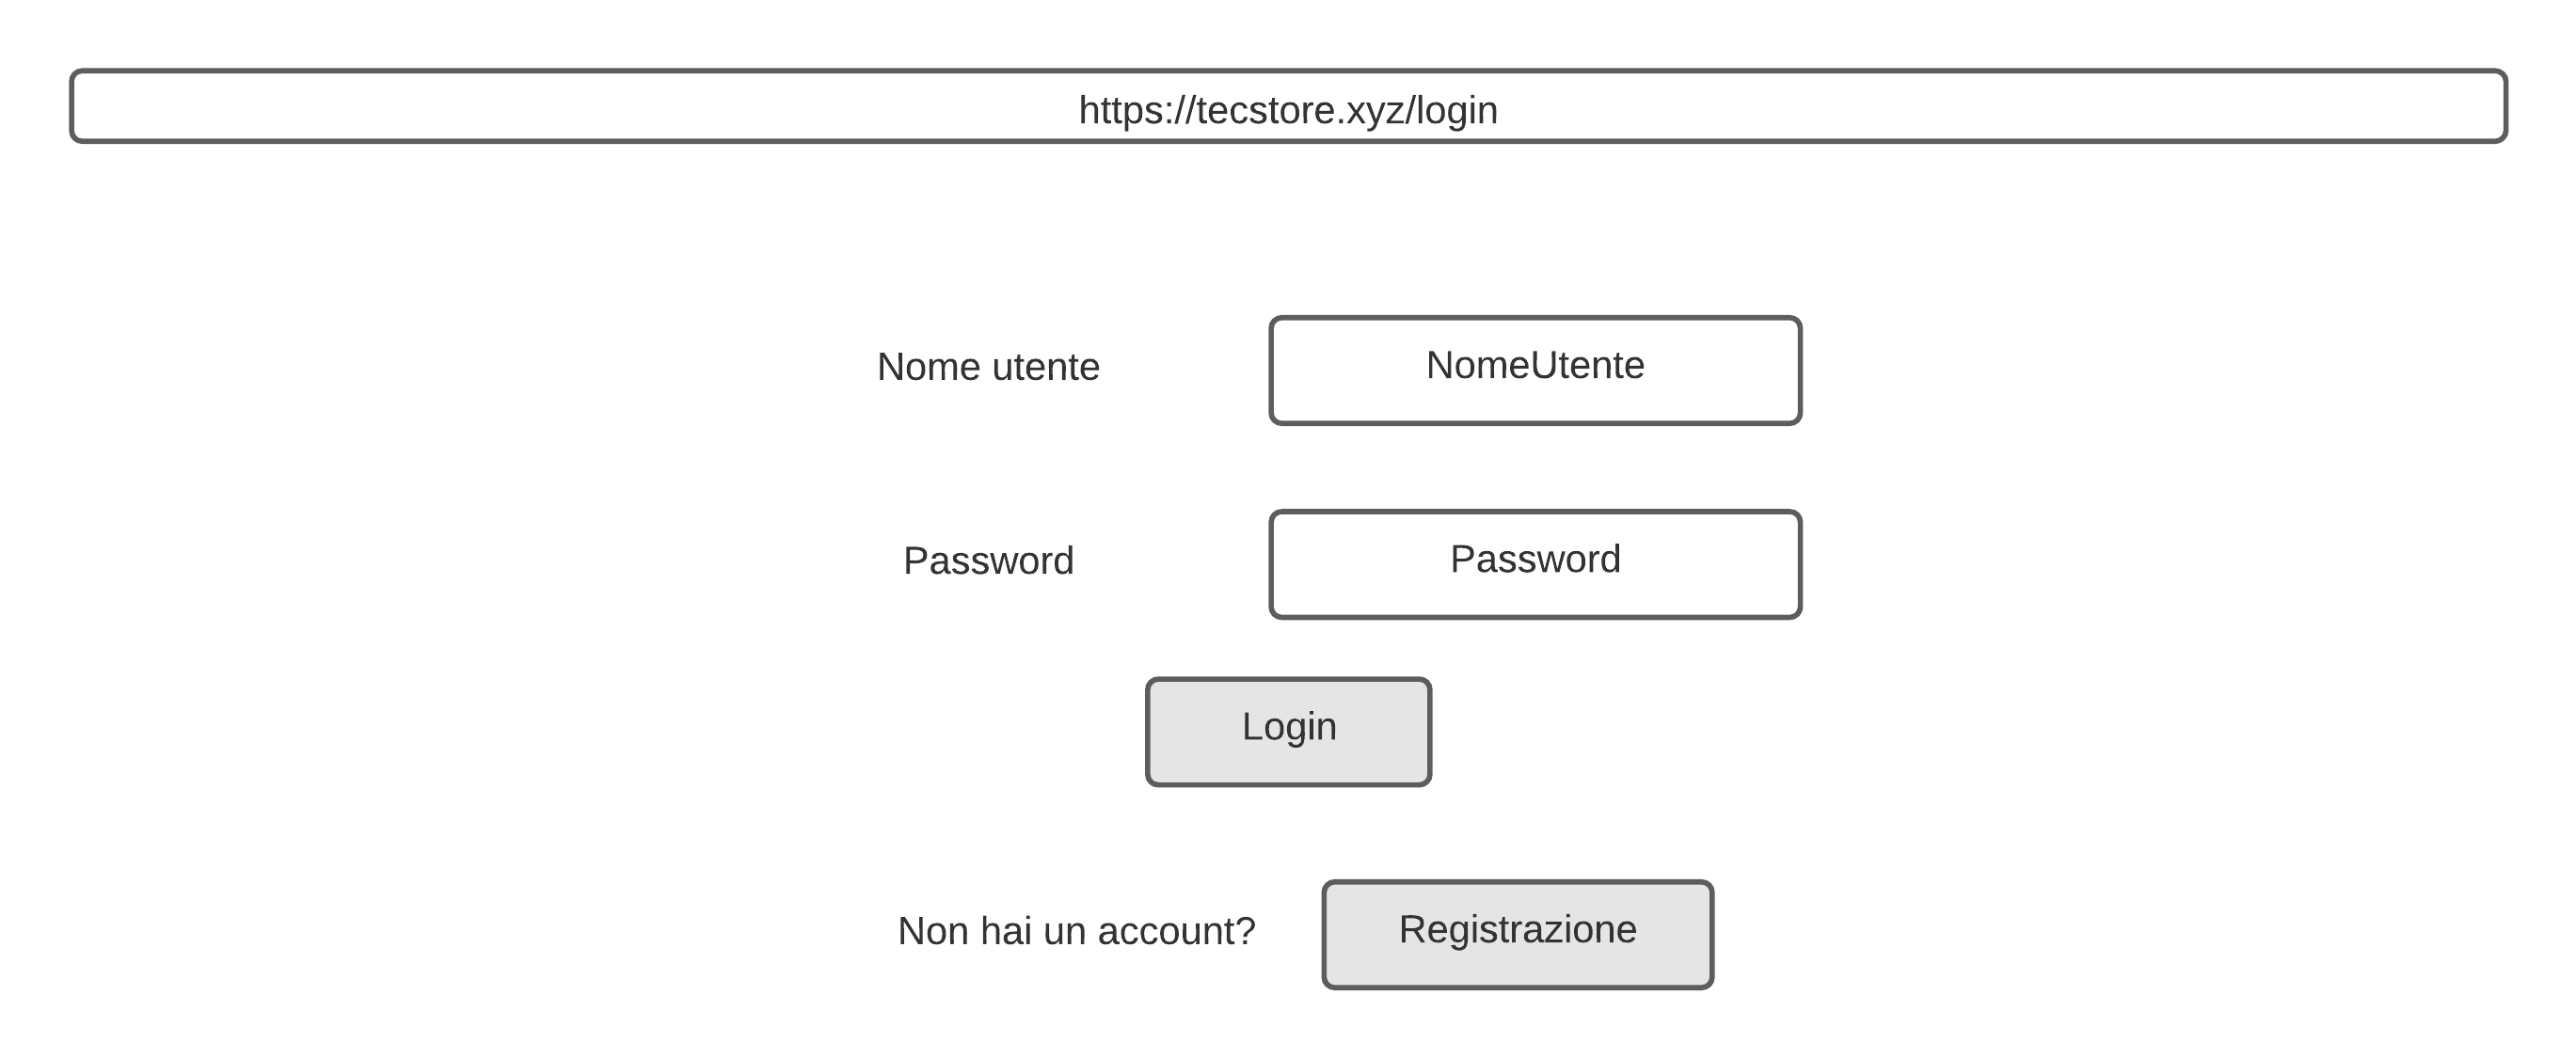
\includegraphics[height=150px]{Mockup/login}

\item Inserisce quindi i suoi dati nel form, "Luca" in nome, "Garibaldi" in cognome, "lucagaribaldi@email.tld" in email, "password1" in password e in conferma password, "20/06/1991" nel campo data di nascita e fa click sul tasto "Conferma". \\

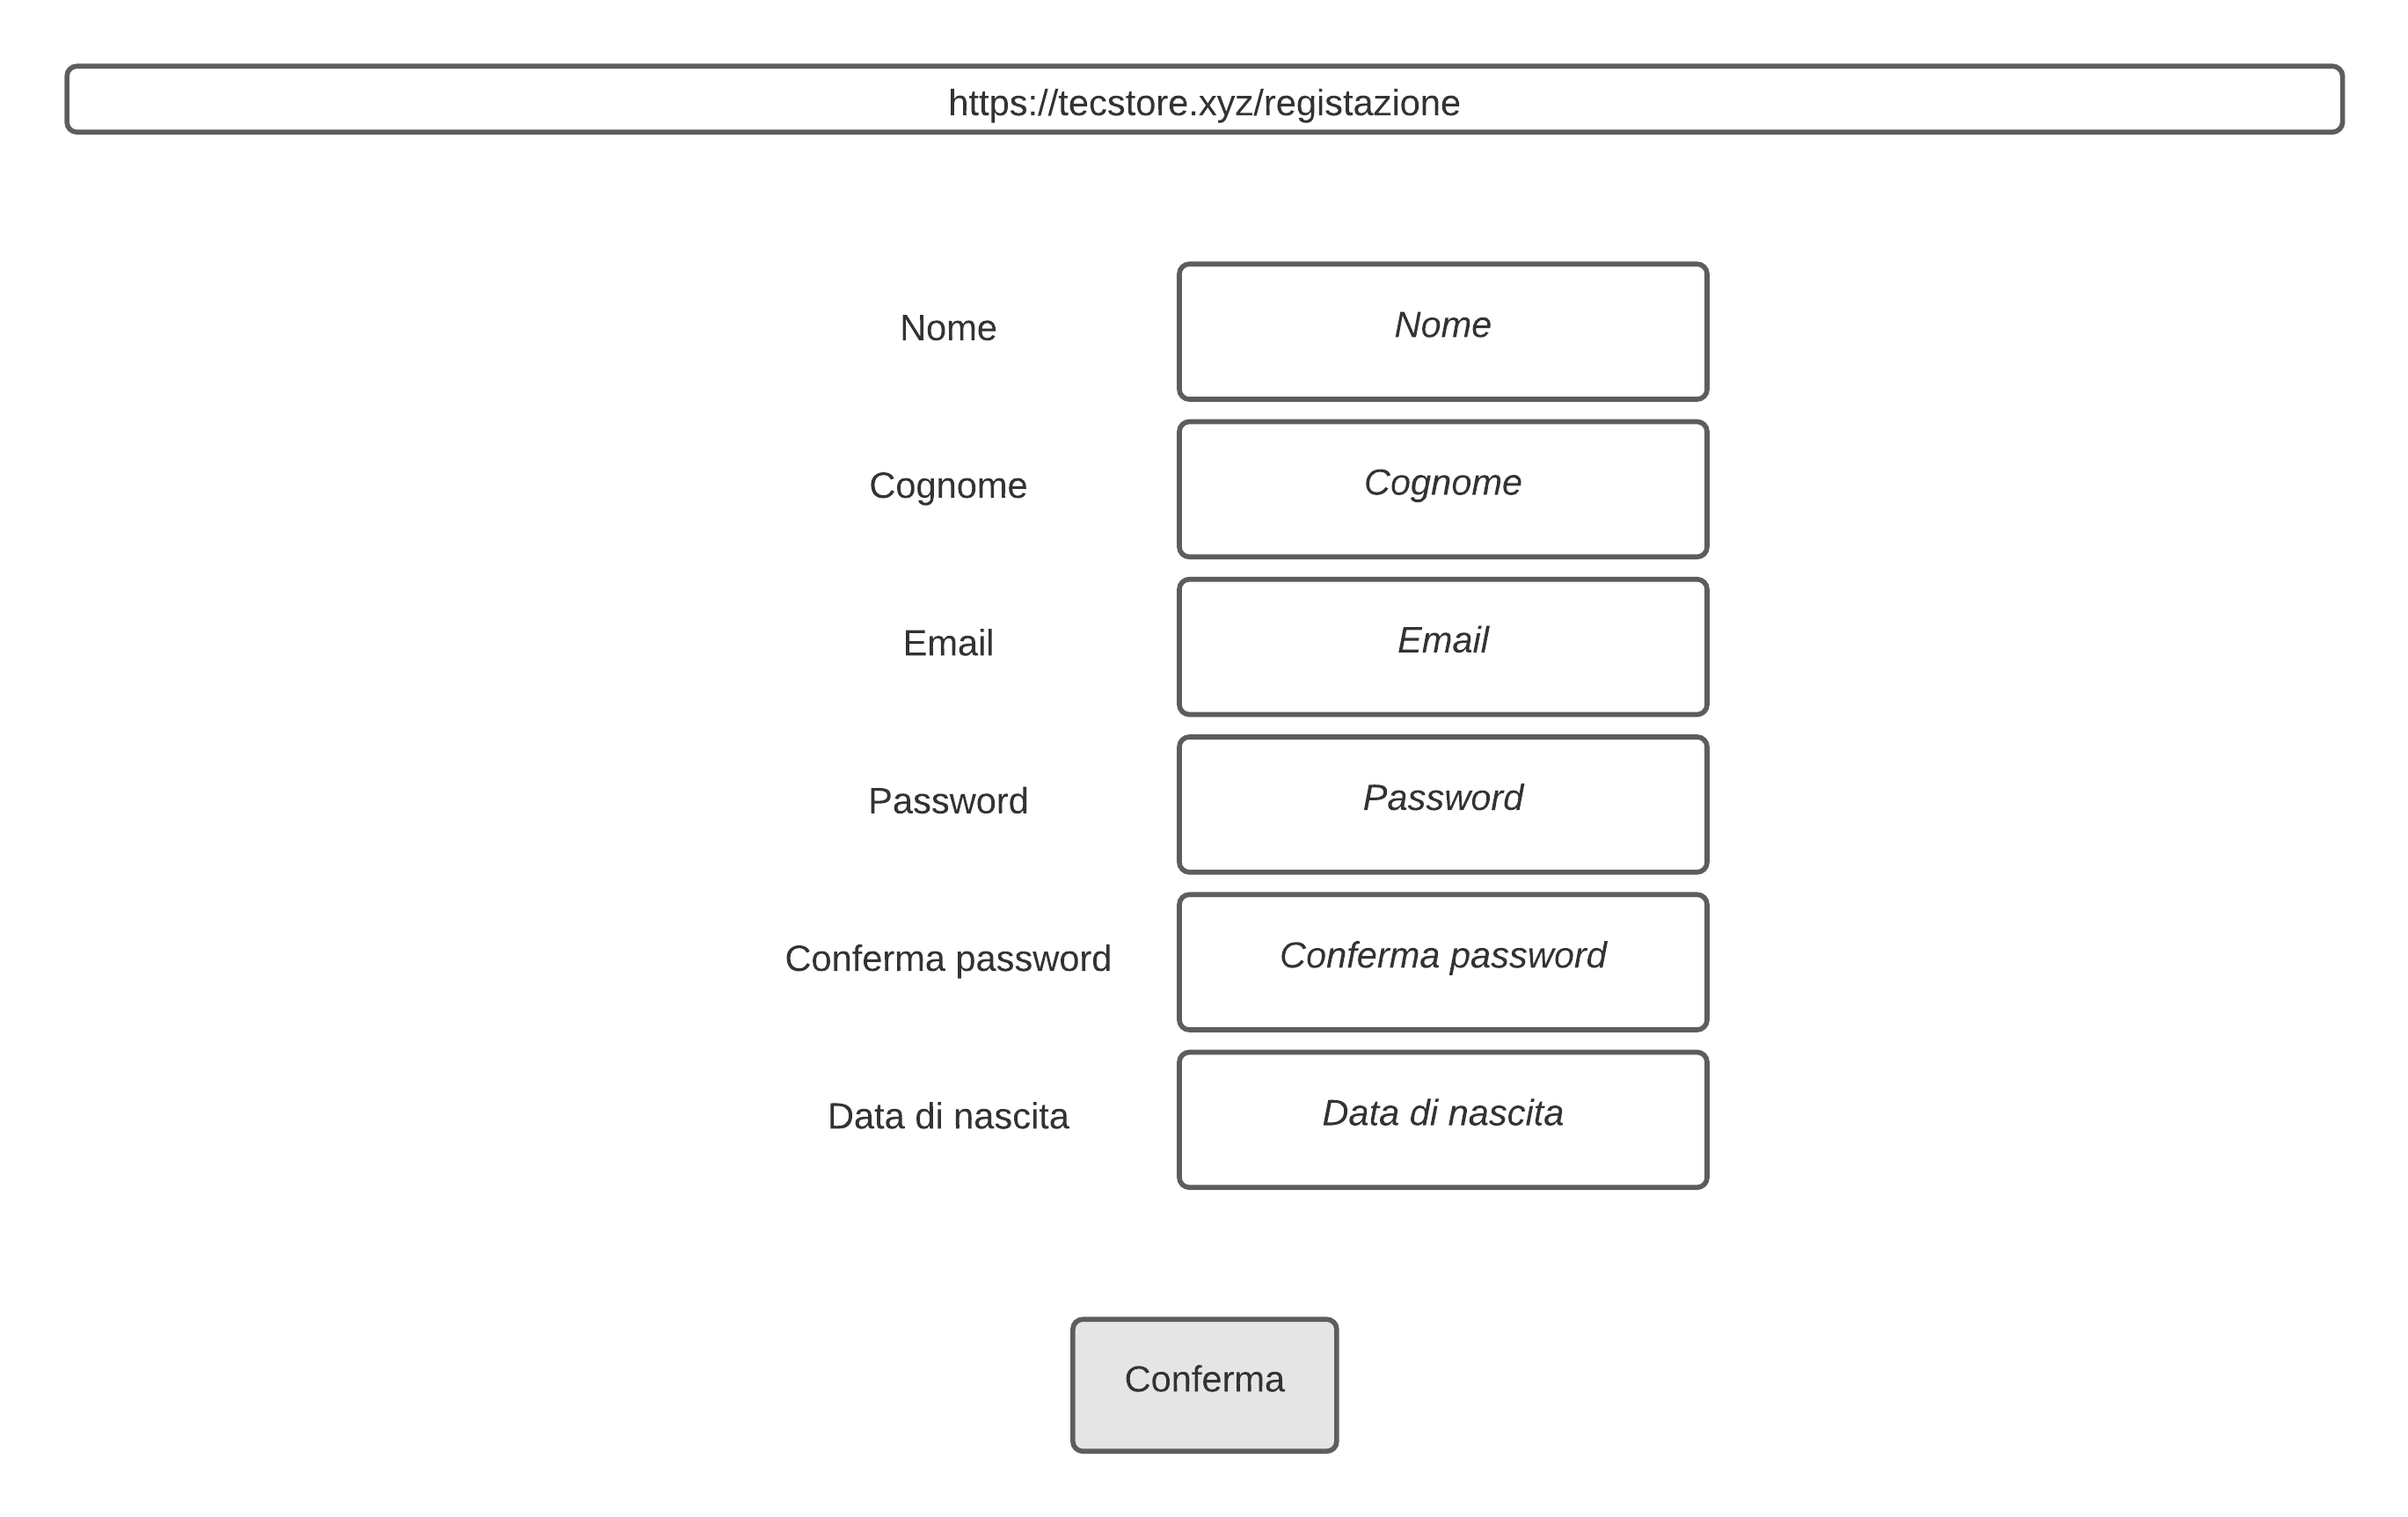
\includegraphics[width=\textwidth]{Mockup/anagrafica}

\newpage
\item Gli vengono chiesti i dati della carta di credito e inserisce "4555133720756196" nel campo numero, 03/23 nel campo scadenza, 356 nel campo CVV, "Via Roma 1" nel campo indirizzo, "Torino 10123" nel campo città, e "Italia" nel campo nazione e fa click sul tasto "Conferma".

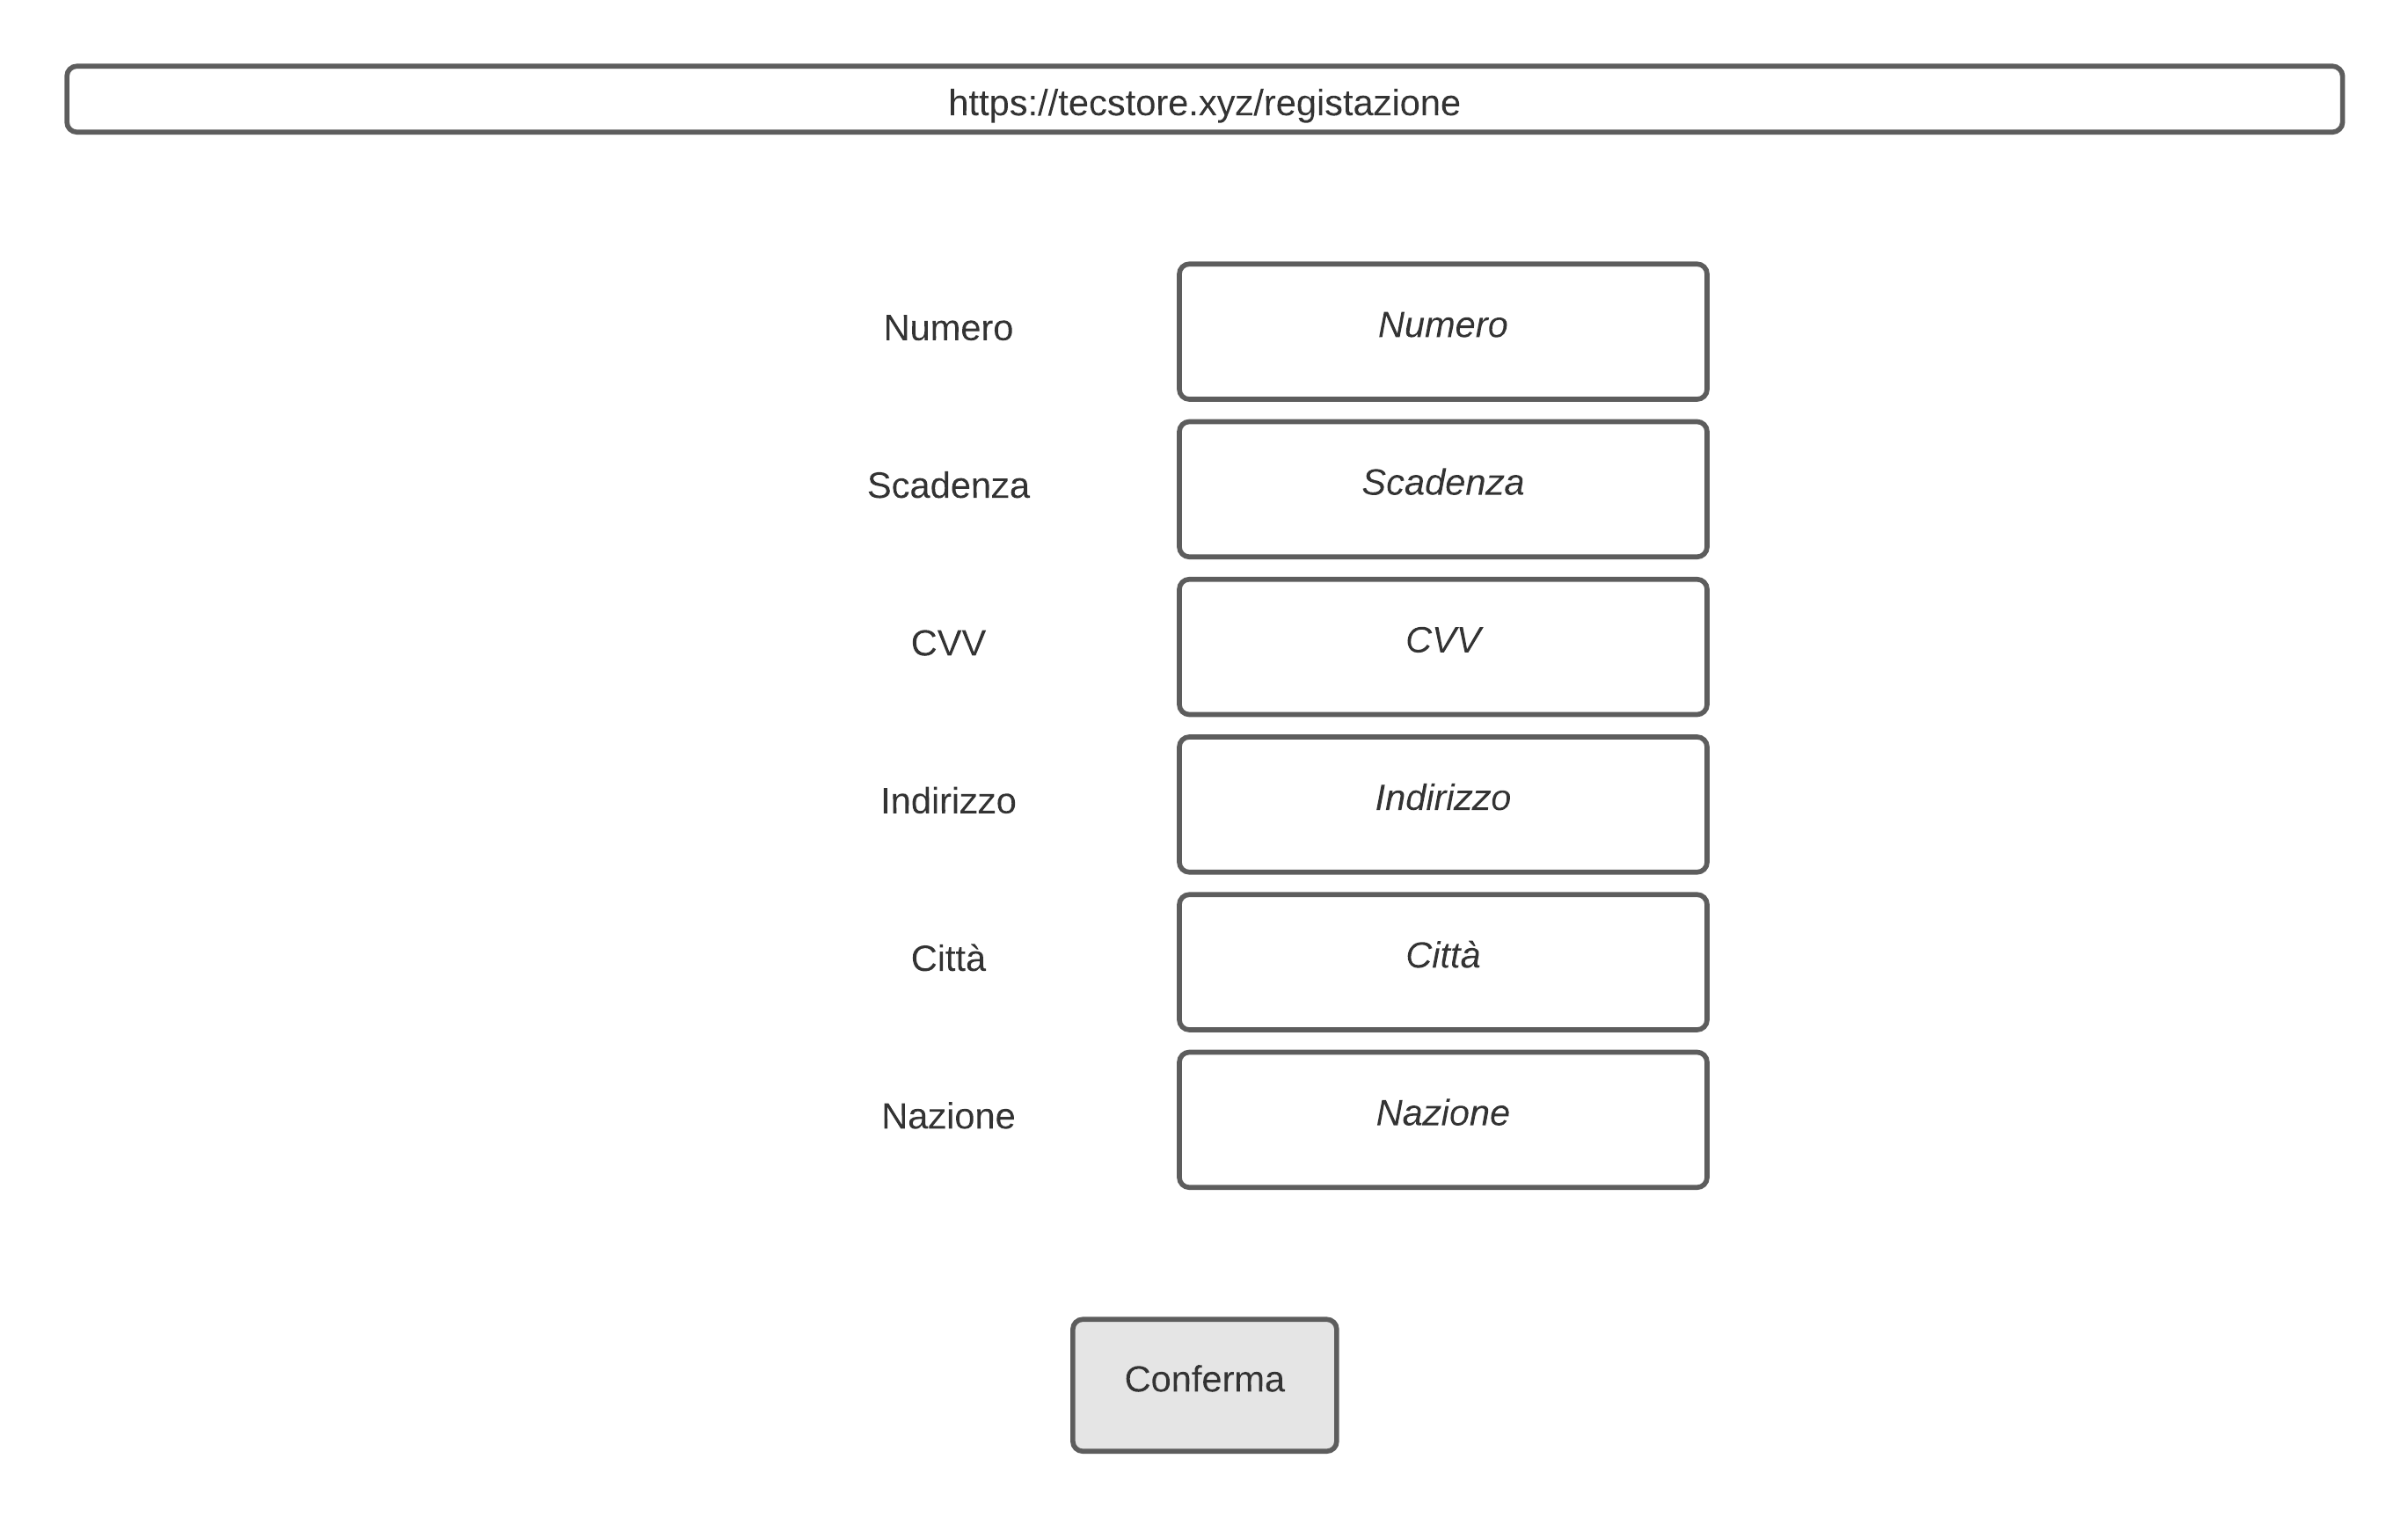
\includegraphics[width=\textwidth]{Mockup/carta}

\item Gli viene chiesta un'ultima conferma prima di effettuare l'ordine. \\
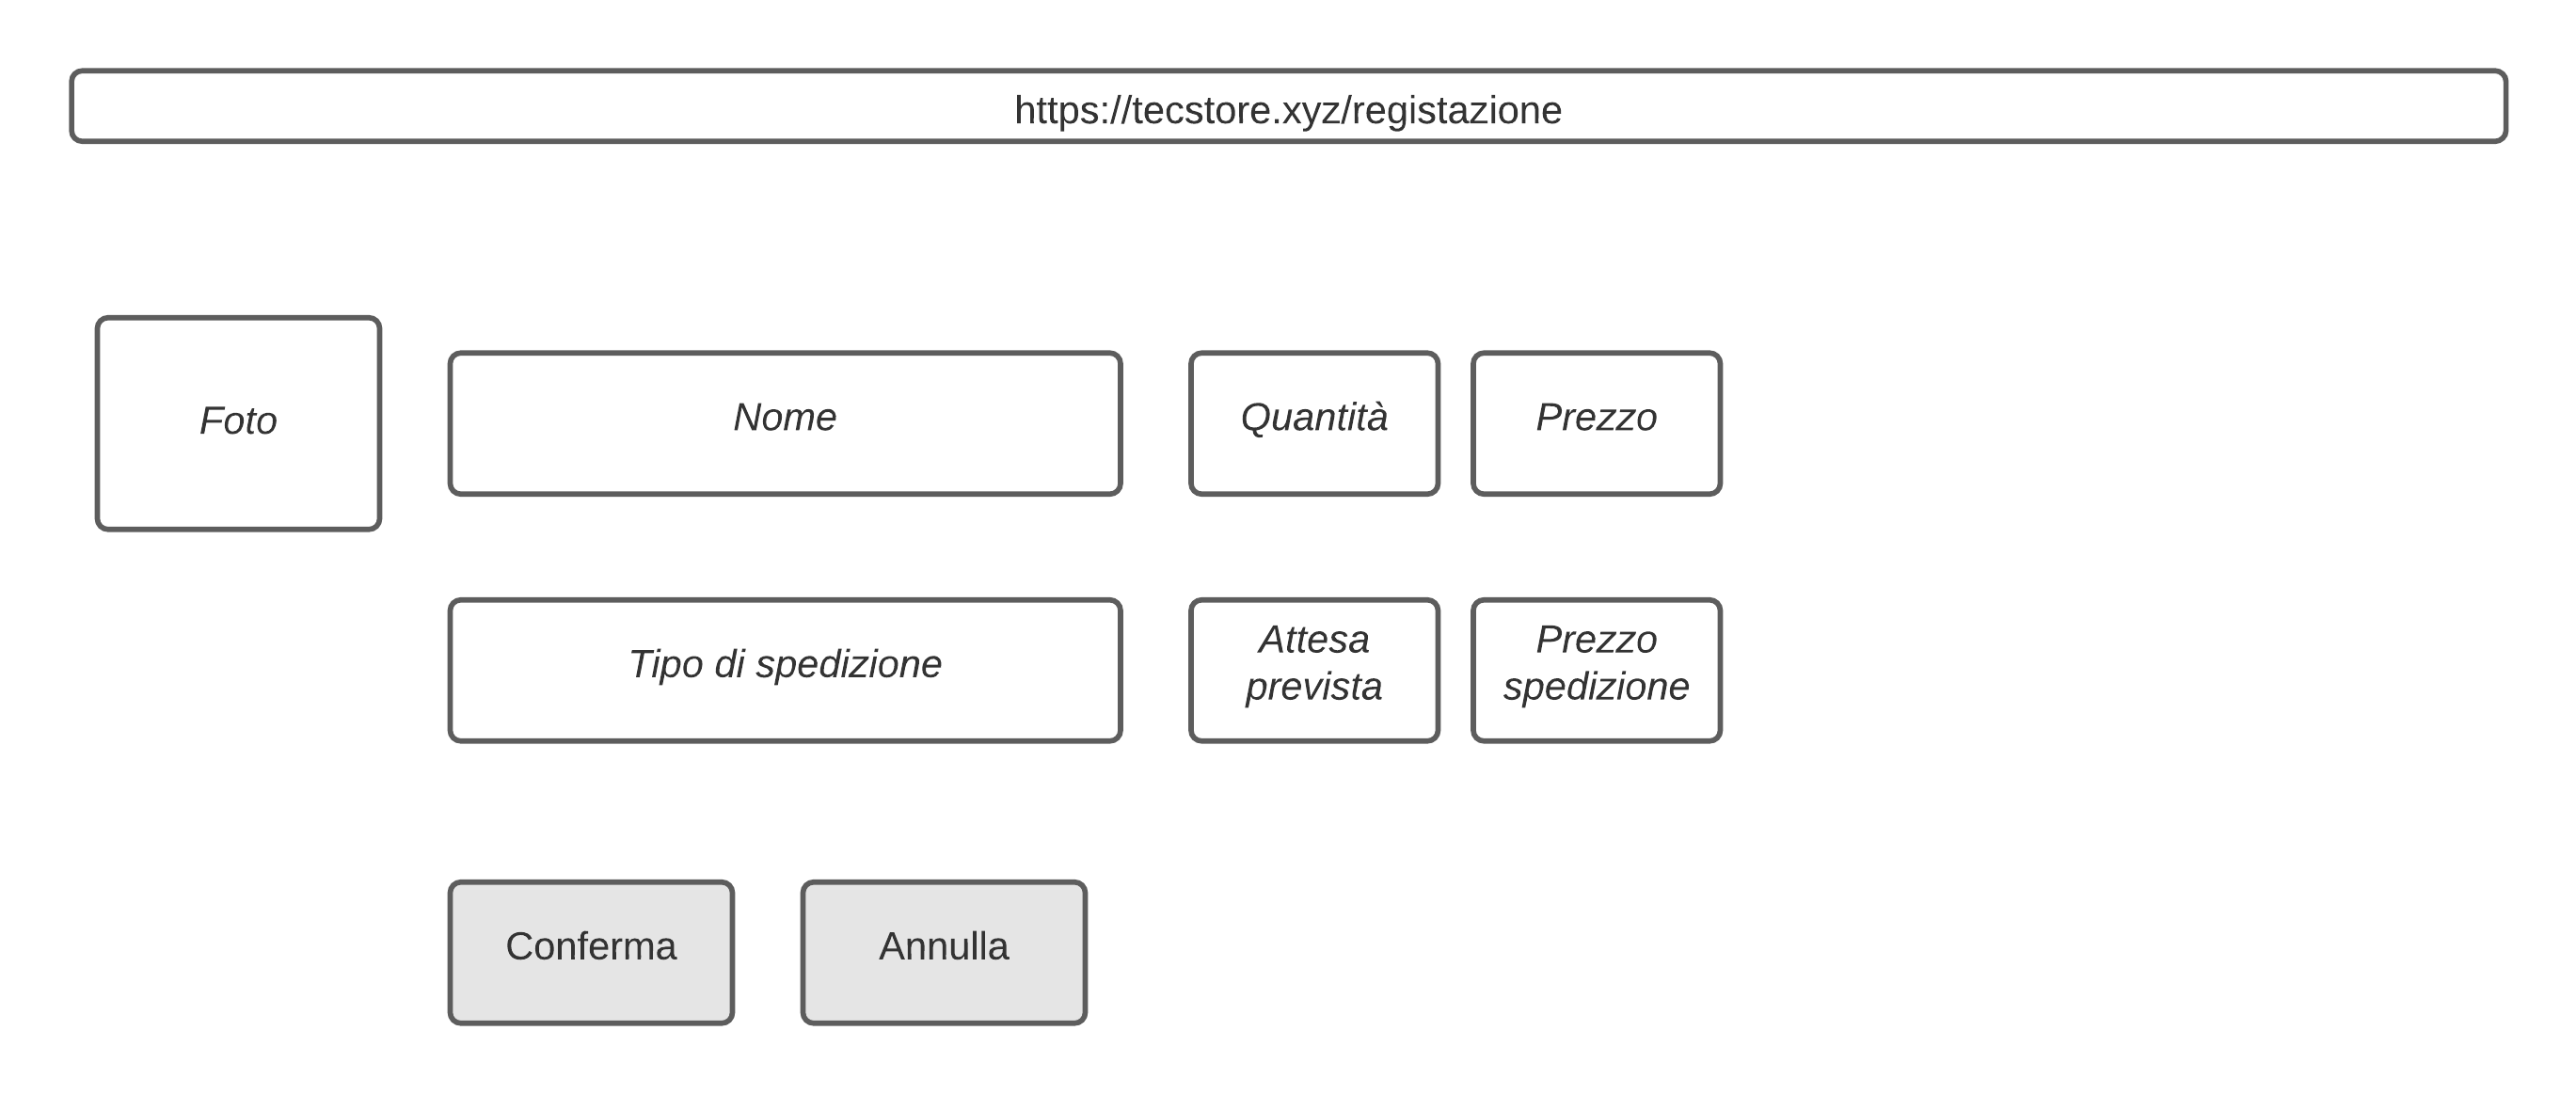
\includegraphics[width=\textwidth]{Mockup/conferma}

\item Al che Luca preme "Acquista".

\item Il mattino dopo, Massimo arriva al lavoro, effettua il login con le credenziali "magazz1" e "0GfbwmXYCIERGT3aU7ja" come password. Vede l'ordine effettuato da Luca, reperisce l'articolo dal magazzino, lo impacchetta, stampa la bolla di spedizione e prenota il corriere per il ritiro dell'articolo.

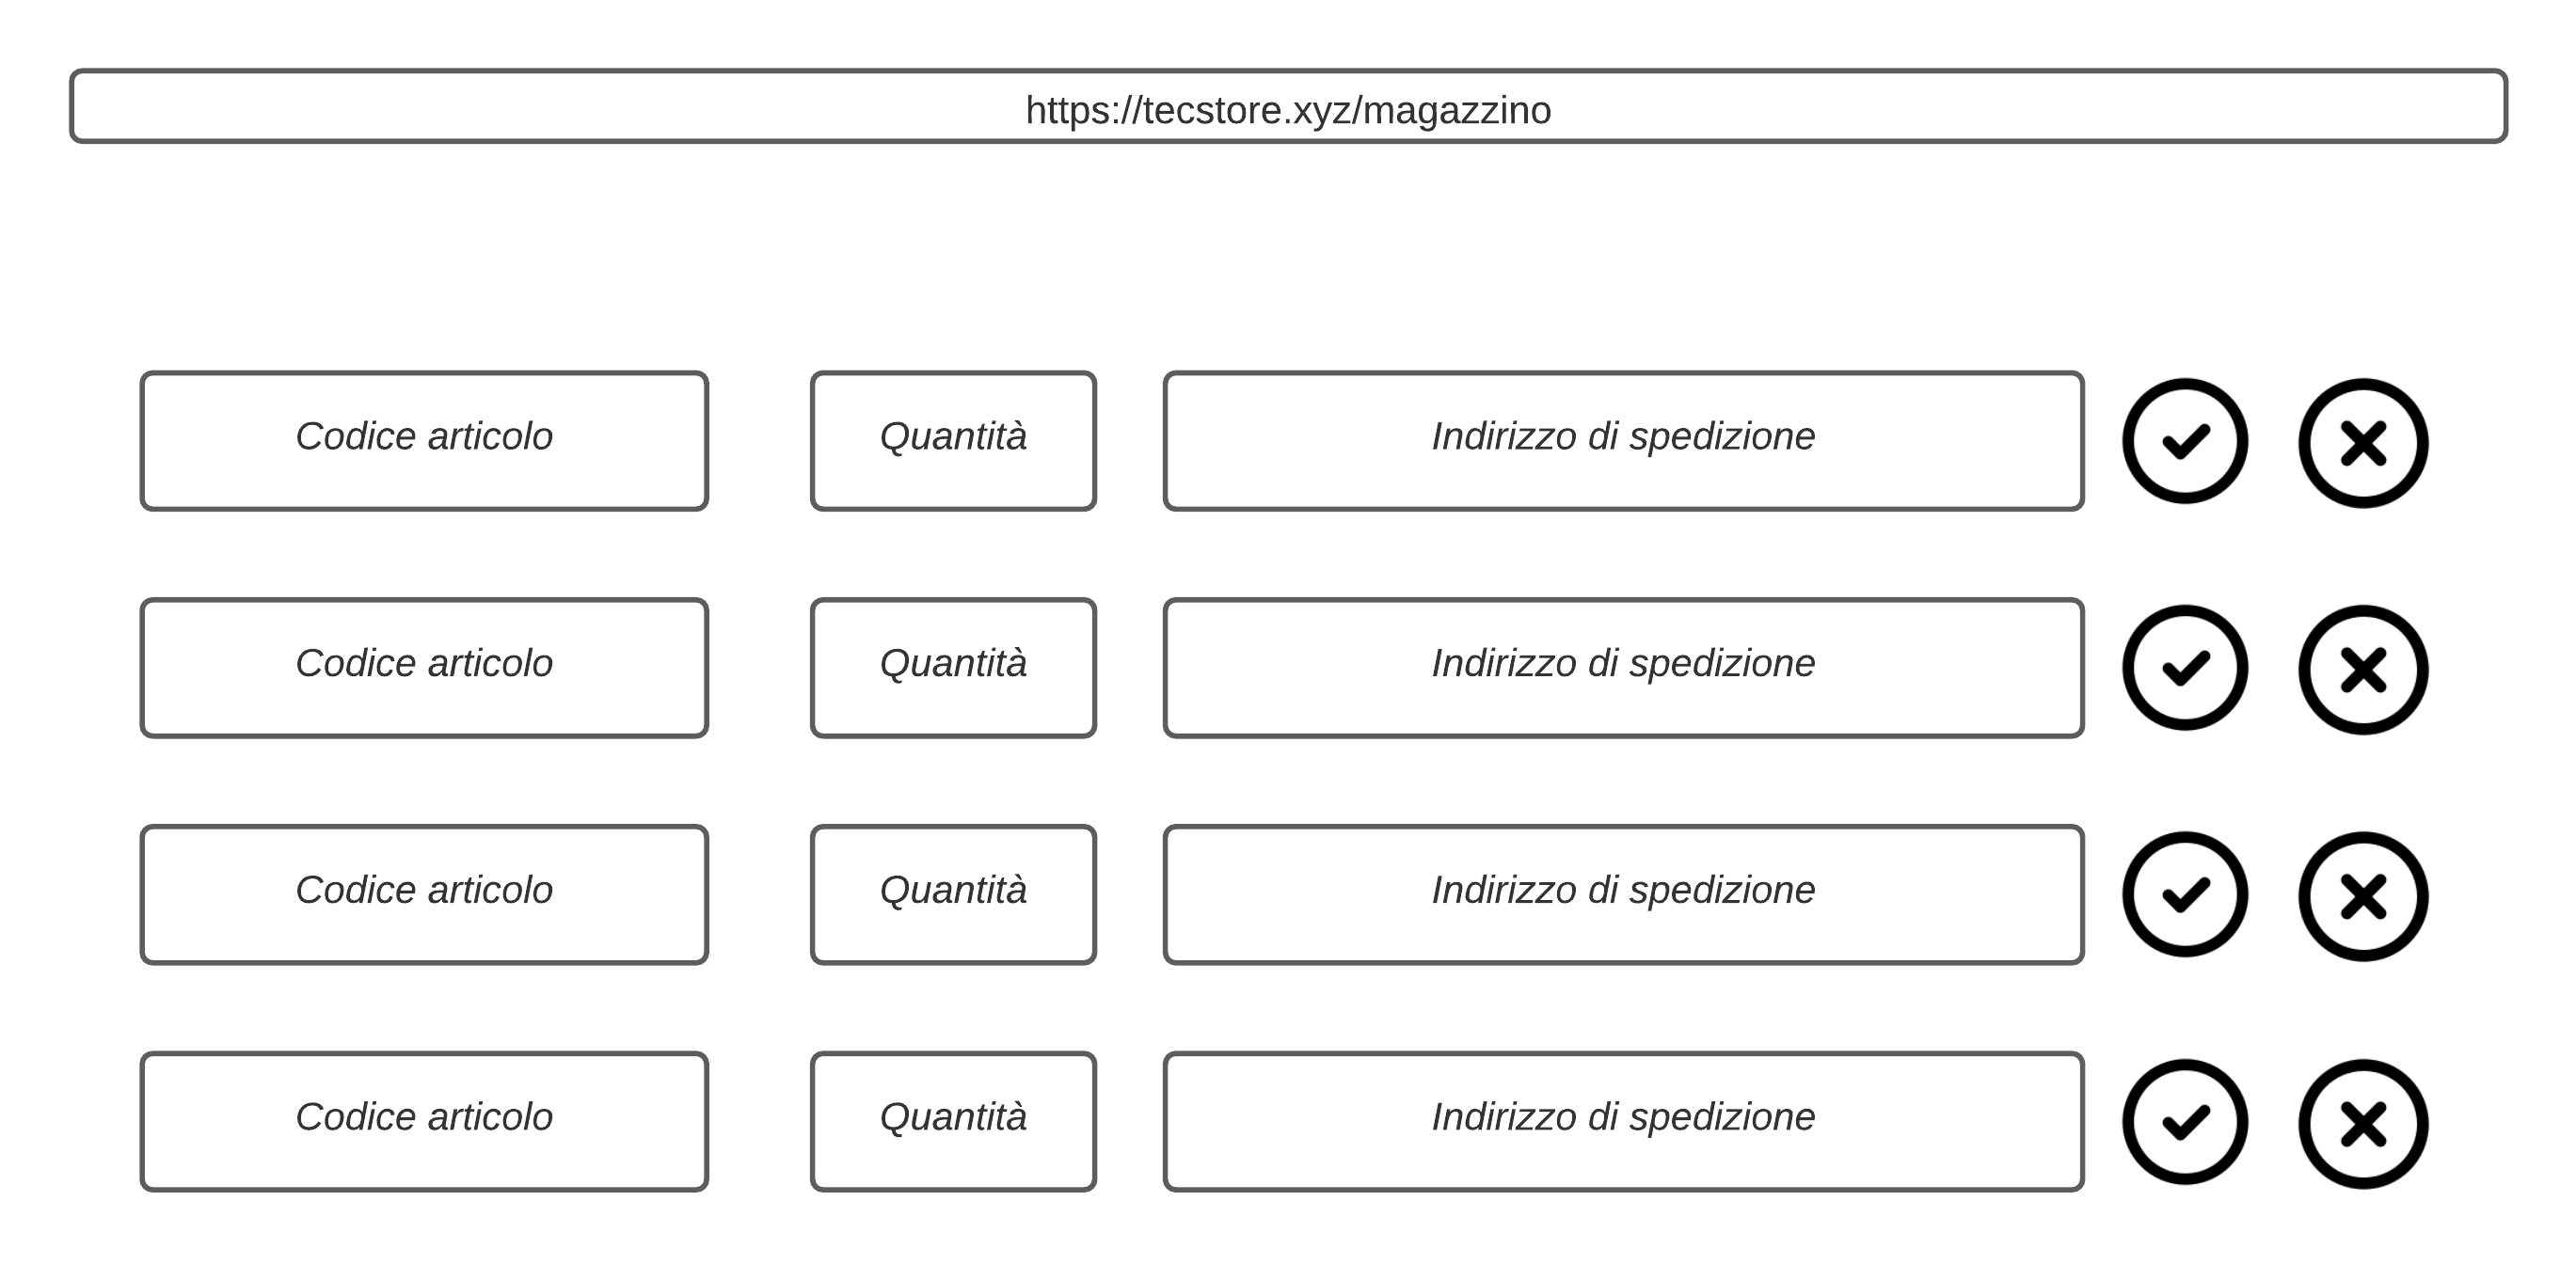
\includegraphics[width=\textwidth]{Mockup/magazzino}

\item Tre giorni dopo un corriere gli consegna l'articolo acquistato.
\end{enumerate}

\newpage
\subsubsection{Un utente apre una segnalazione all'assistenza}
\textbf{Attori:} Carlo Cavour, utente e Lucia Pellegrino, centralinista \\
\noindent
\textbf{Flusso di eventi:}
\begin{enumerate}
\item 10 giorni fa Carlo ha ordinato un nuovo hard disk, ma non l'ha ancora ricevuto. Decide quindi di aprire un ticket su TecStore.

\item Apre la homepage del sito. \\

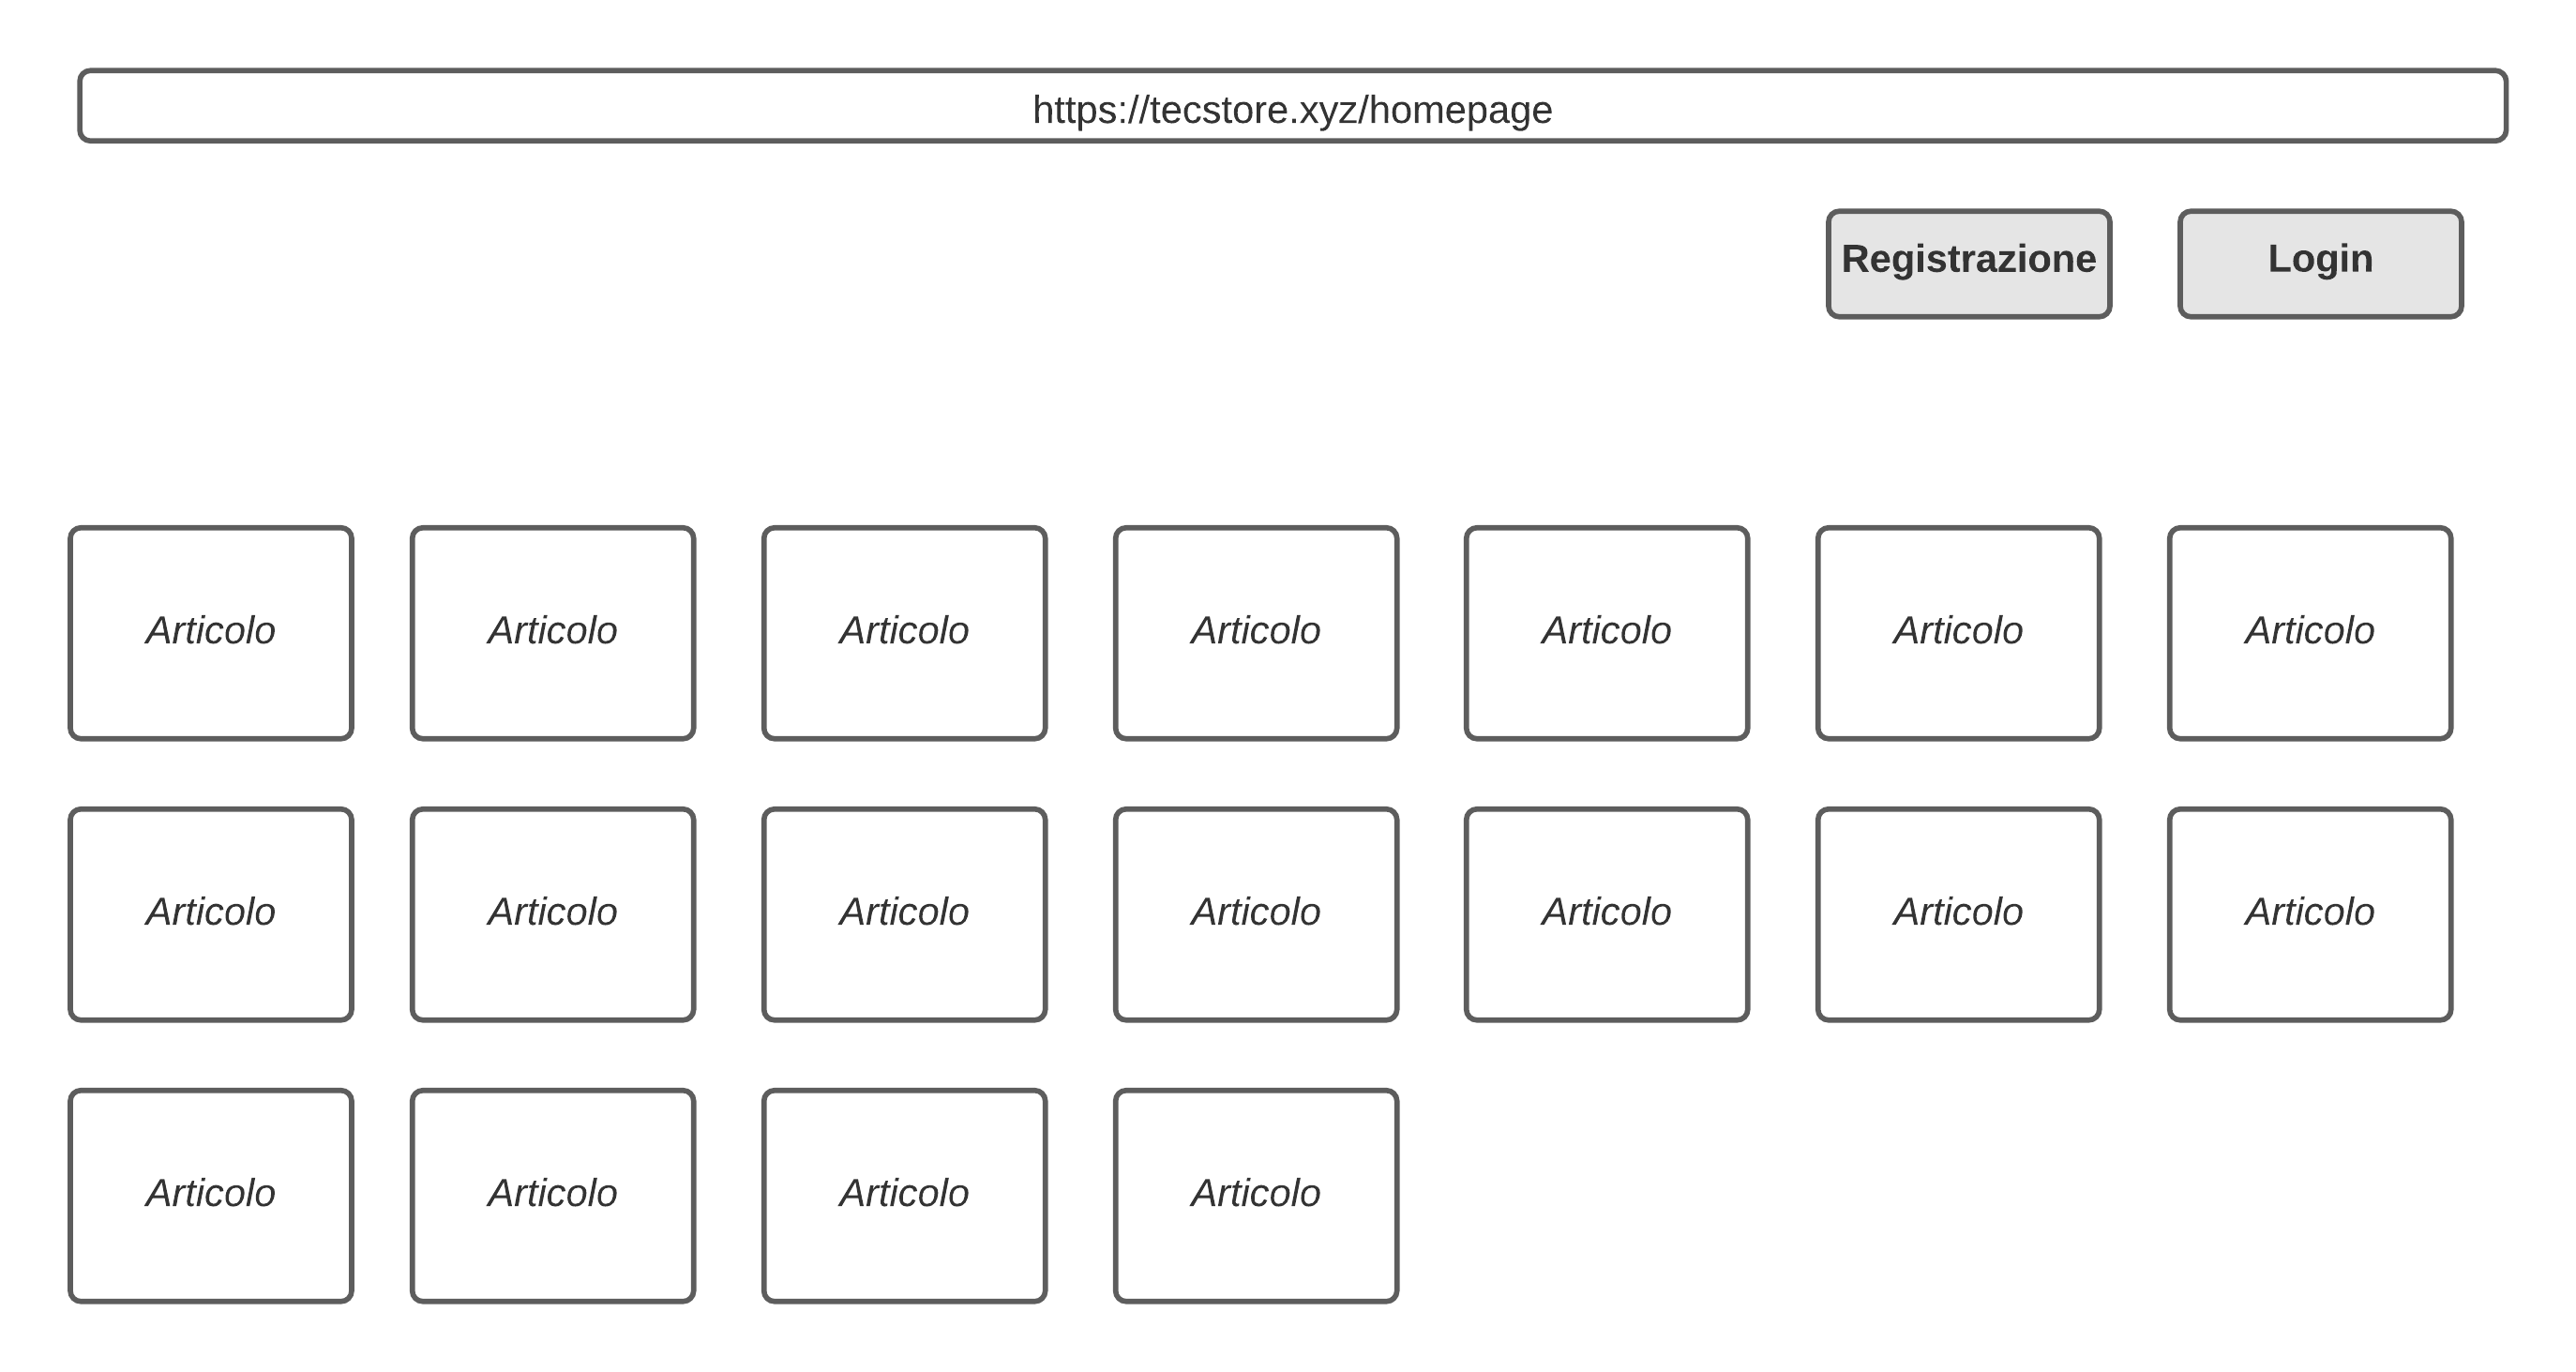
\includegraphics[width=\textwidth]{Mockup/homepage}

\item Fa click sul tasto "Login" e viene riportato al form in cui gli viene chiesto di inserire email e password, inserisce rispettivamente \\ "carlocavour@email.tld" e "hunter2" e fa click sul tasto per confermare.

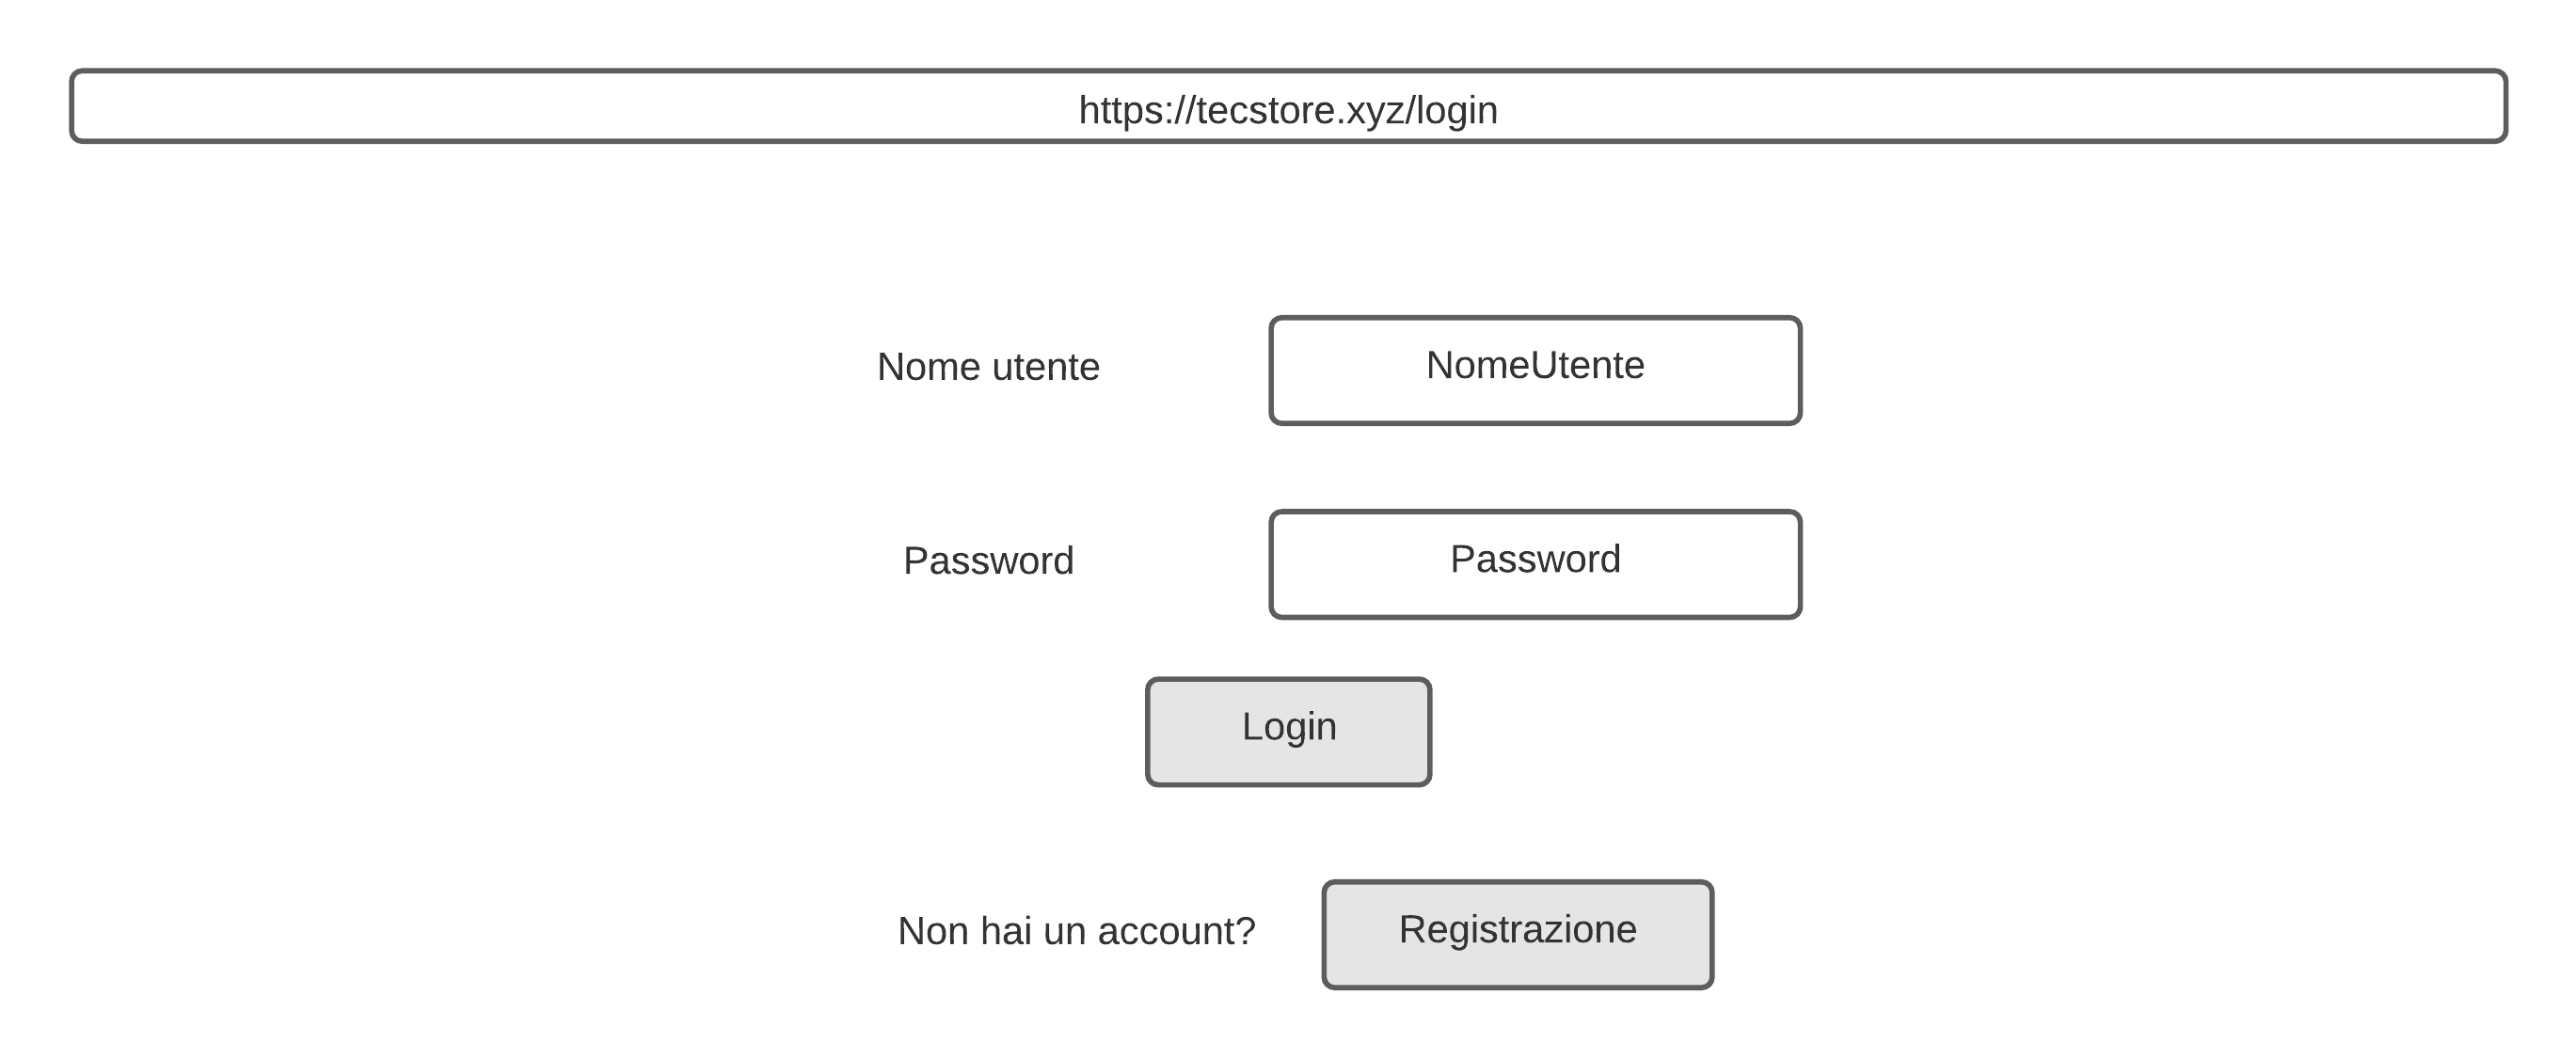
\includegraphics[height=150px]{Mockup/login}

\newpage
\item Viene quindi reindirizzato all'interfaccia principale. Passa il mouse sul suo nome e fa click sul tasto "Assistenza clienti".

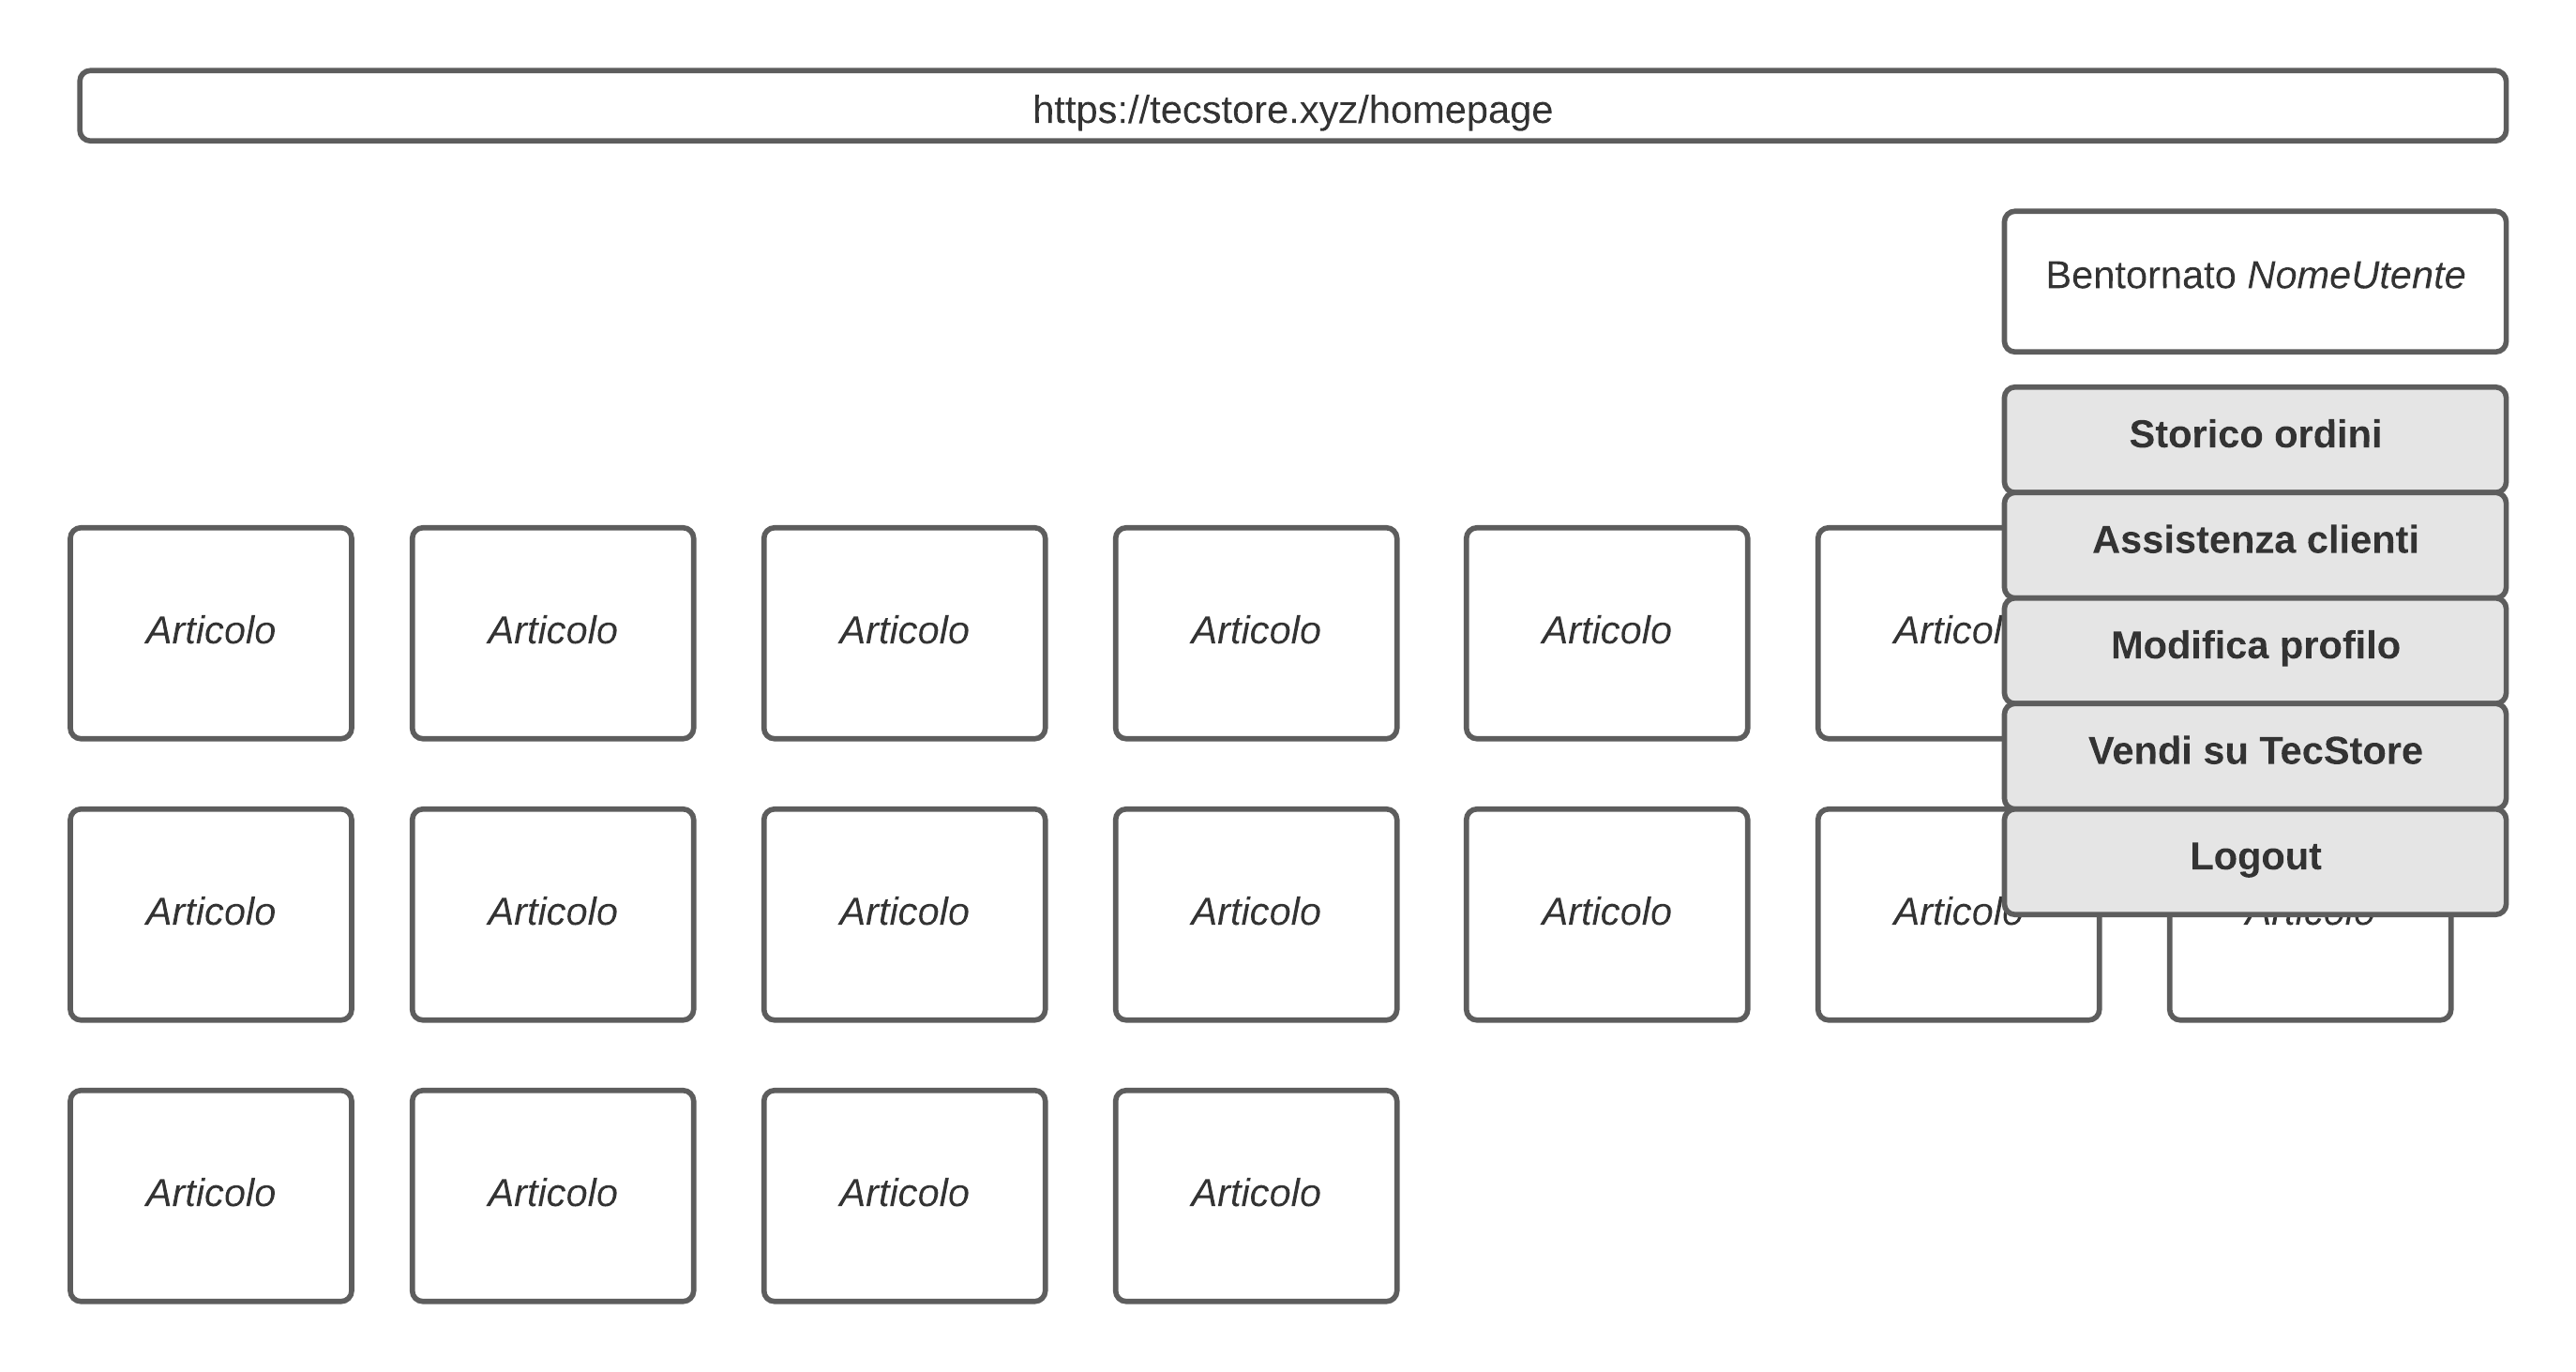
\includegraphics[width=\textwidth]{Mockup/homepage_login}

\item Viene portato nella pagina per la creazione di un nuovo ticket, sceglie "Problemi di spedizione" come tipologia e scrive "Non ho ricevuto il mio articolo dopo 10 giorni" nel campo descrizione. \\
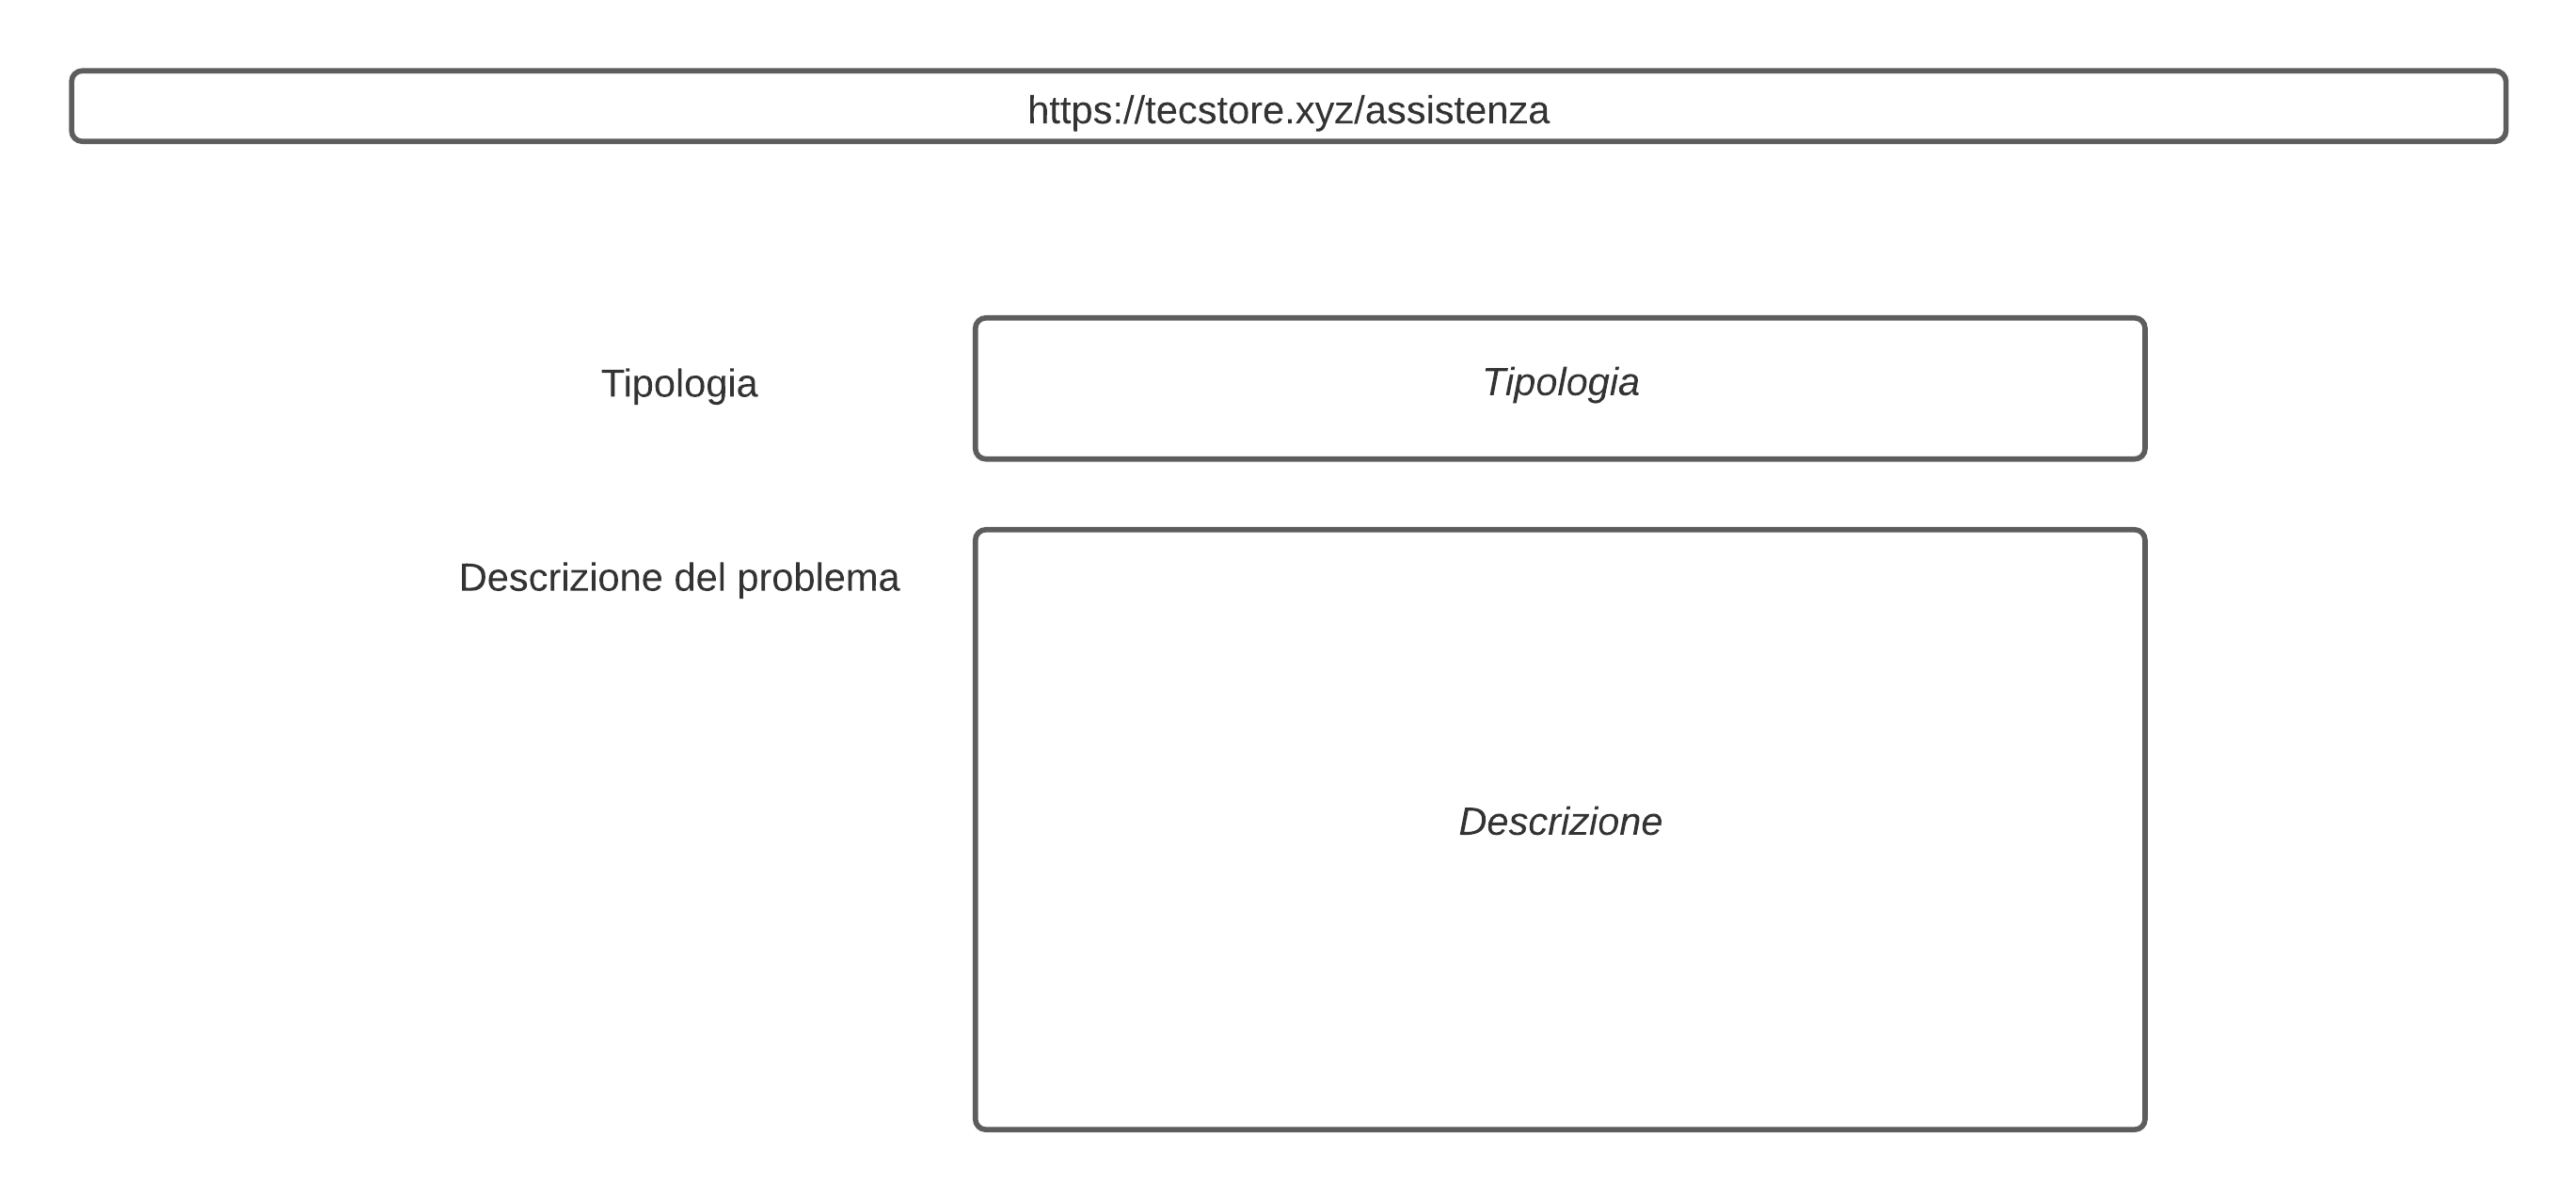
\includegraphics[width=\textwidth]{Mockup/assistenza}

\newpage
\item Lucia effettua il login, vede il nuovo ticket e risponde a Carlo che nei giorni precedenti ci sono stati problemi con il corriere che TecStore solitamente utilizza per spedire gli articoli e lo assicura che riceverà l'articolo entro le successive 48 ore.

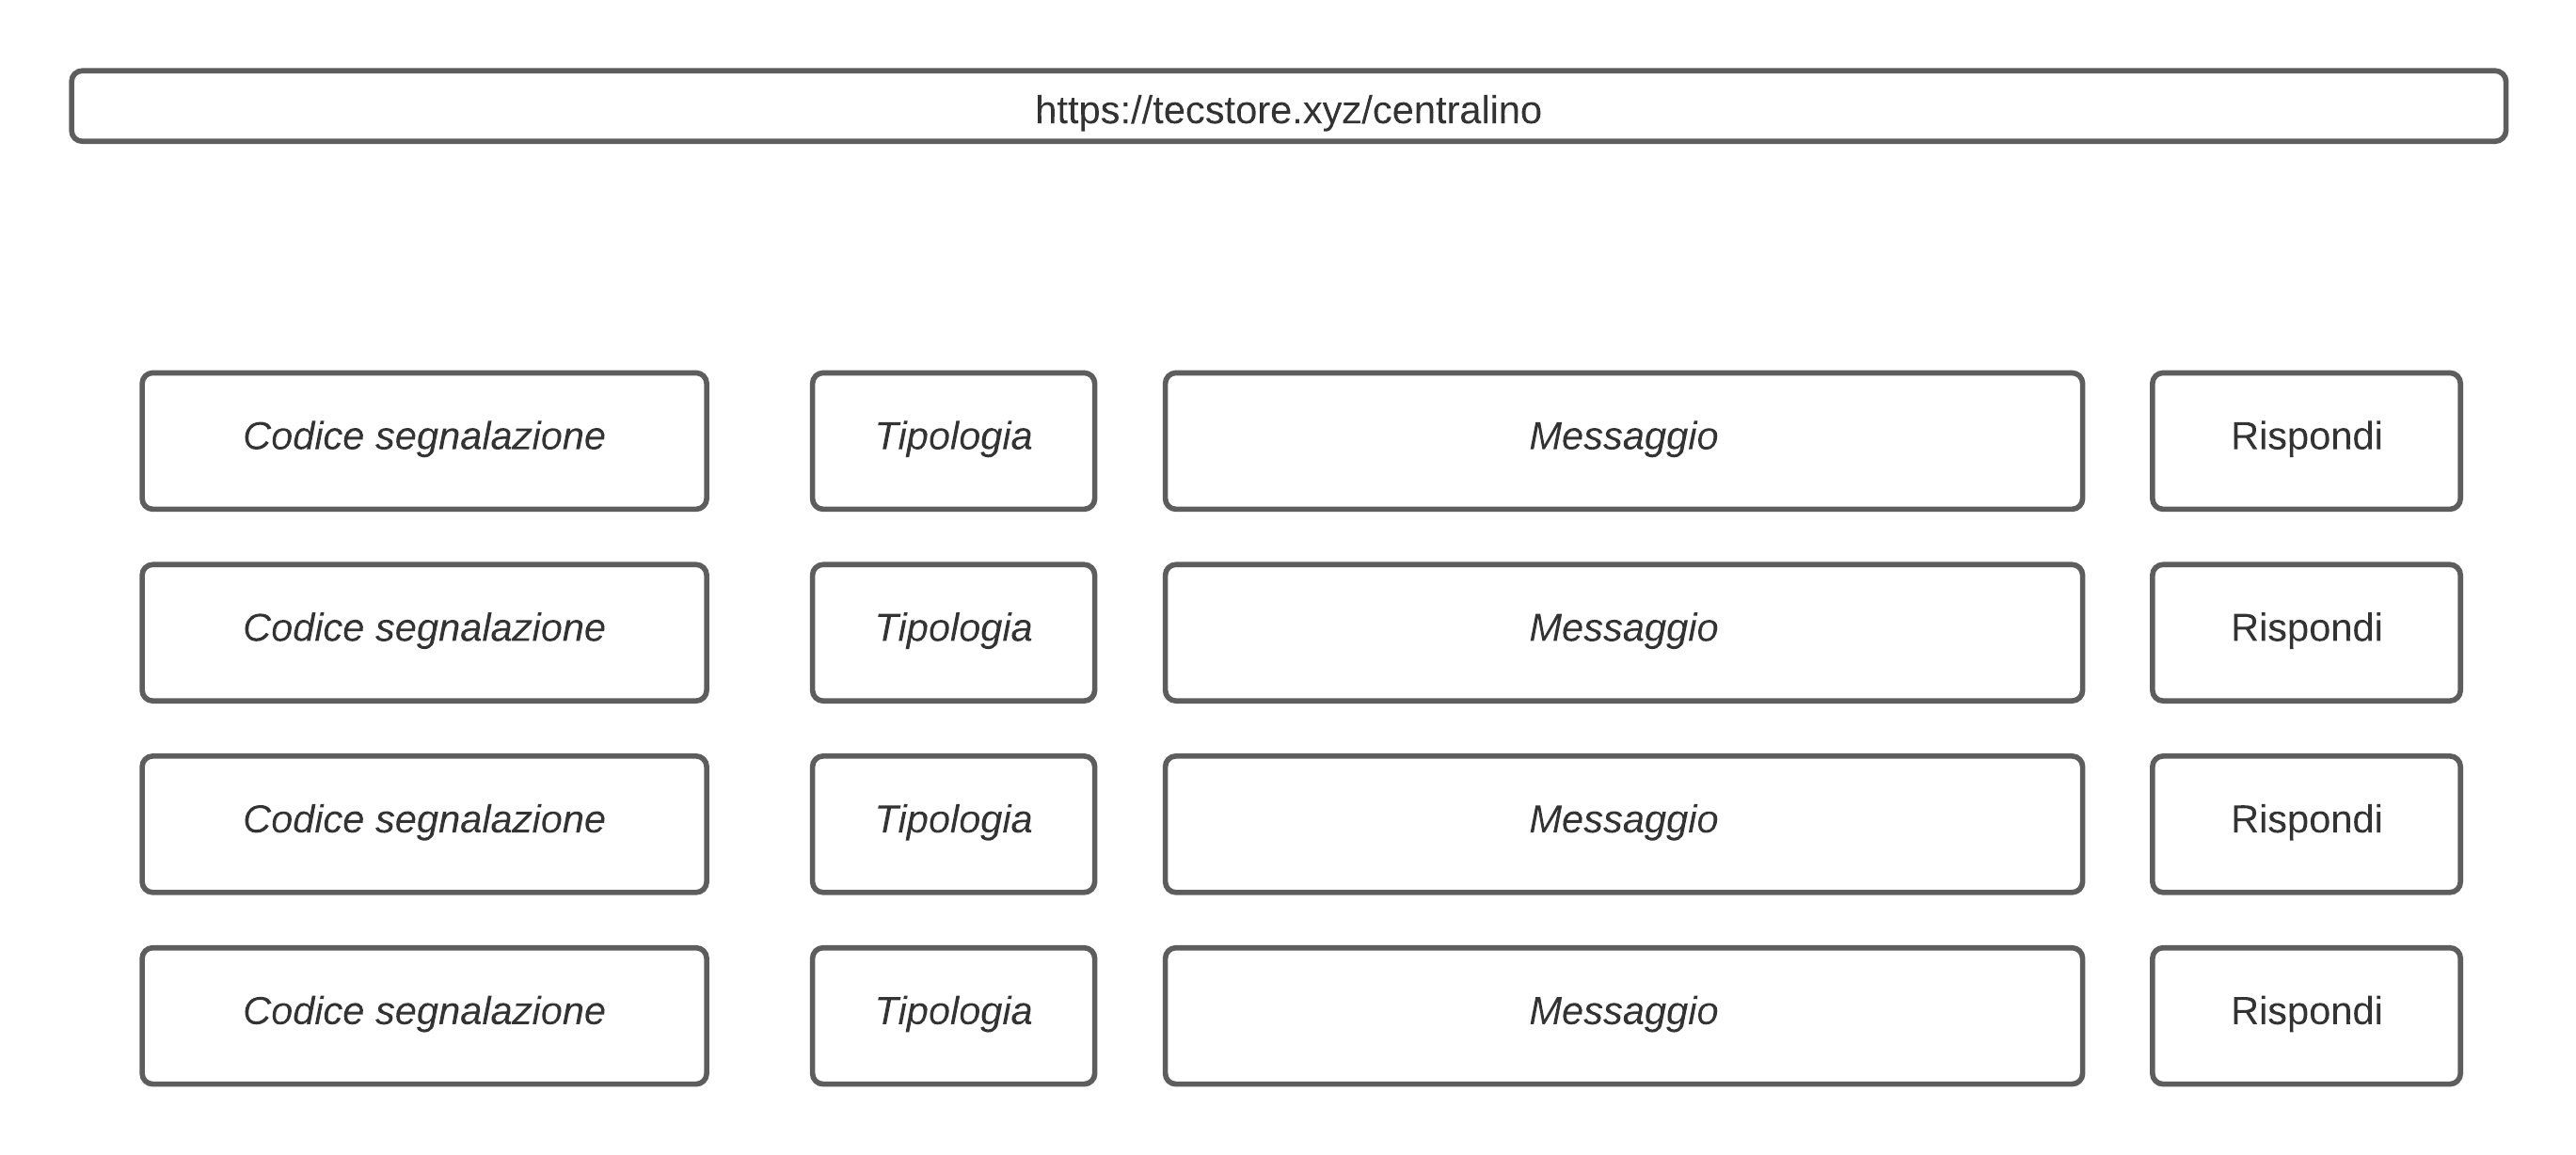
\includegraphics[width=\textwidth]{Mockup/centralino}

\item La mattina del giorno dopo Carlo riceve l'articolo ordinato.
\end{enumerate}

\subsubsection{Un utente vuole mettere in vendita un articolo}
\textbf{Attori:} Alfonso Siciliani, utente e Silvana Piazza, centralinista \\

\noindent
\textbf{Flusso di eventi:}

\begin{enumerate}

\item Alfonso ha un piccolo negozio di informatica e ha un surplus di monitor che non riesce a vendere nel suo negozio. Decide quindi di metterli in vendita online.

\item Per ampliare la potenziale utenza, oltre a piattaforme più note, decide di inserirlo anche in qualche sito meno conosciuto e sceglie tra le possibili opzioni anche TecStore.
\newpage

\item Essendo un utente già registrato, apre la homepage, clicka sul link "Login".

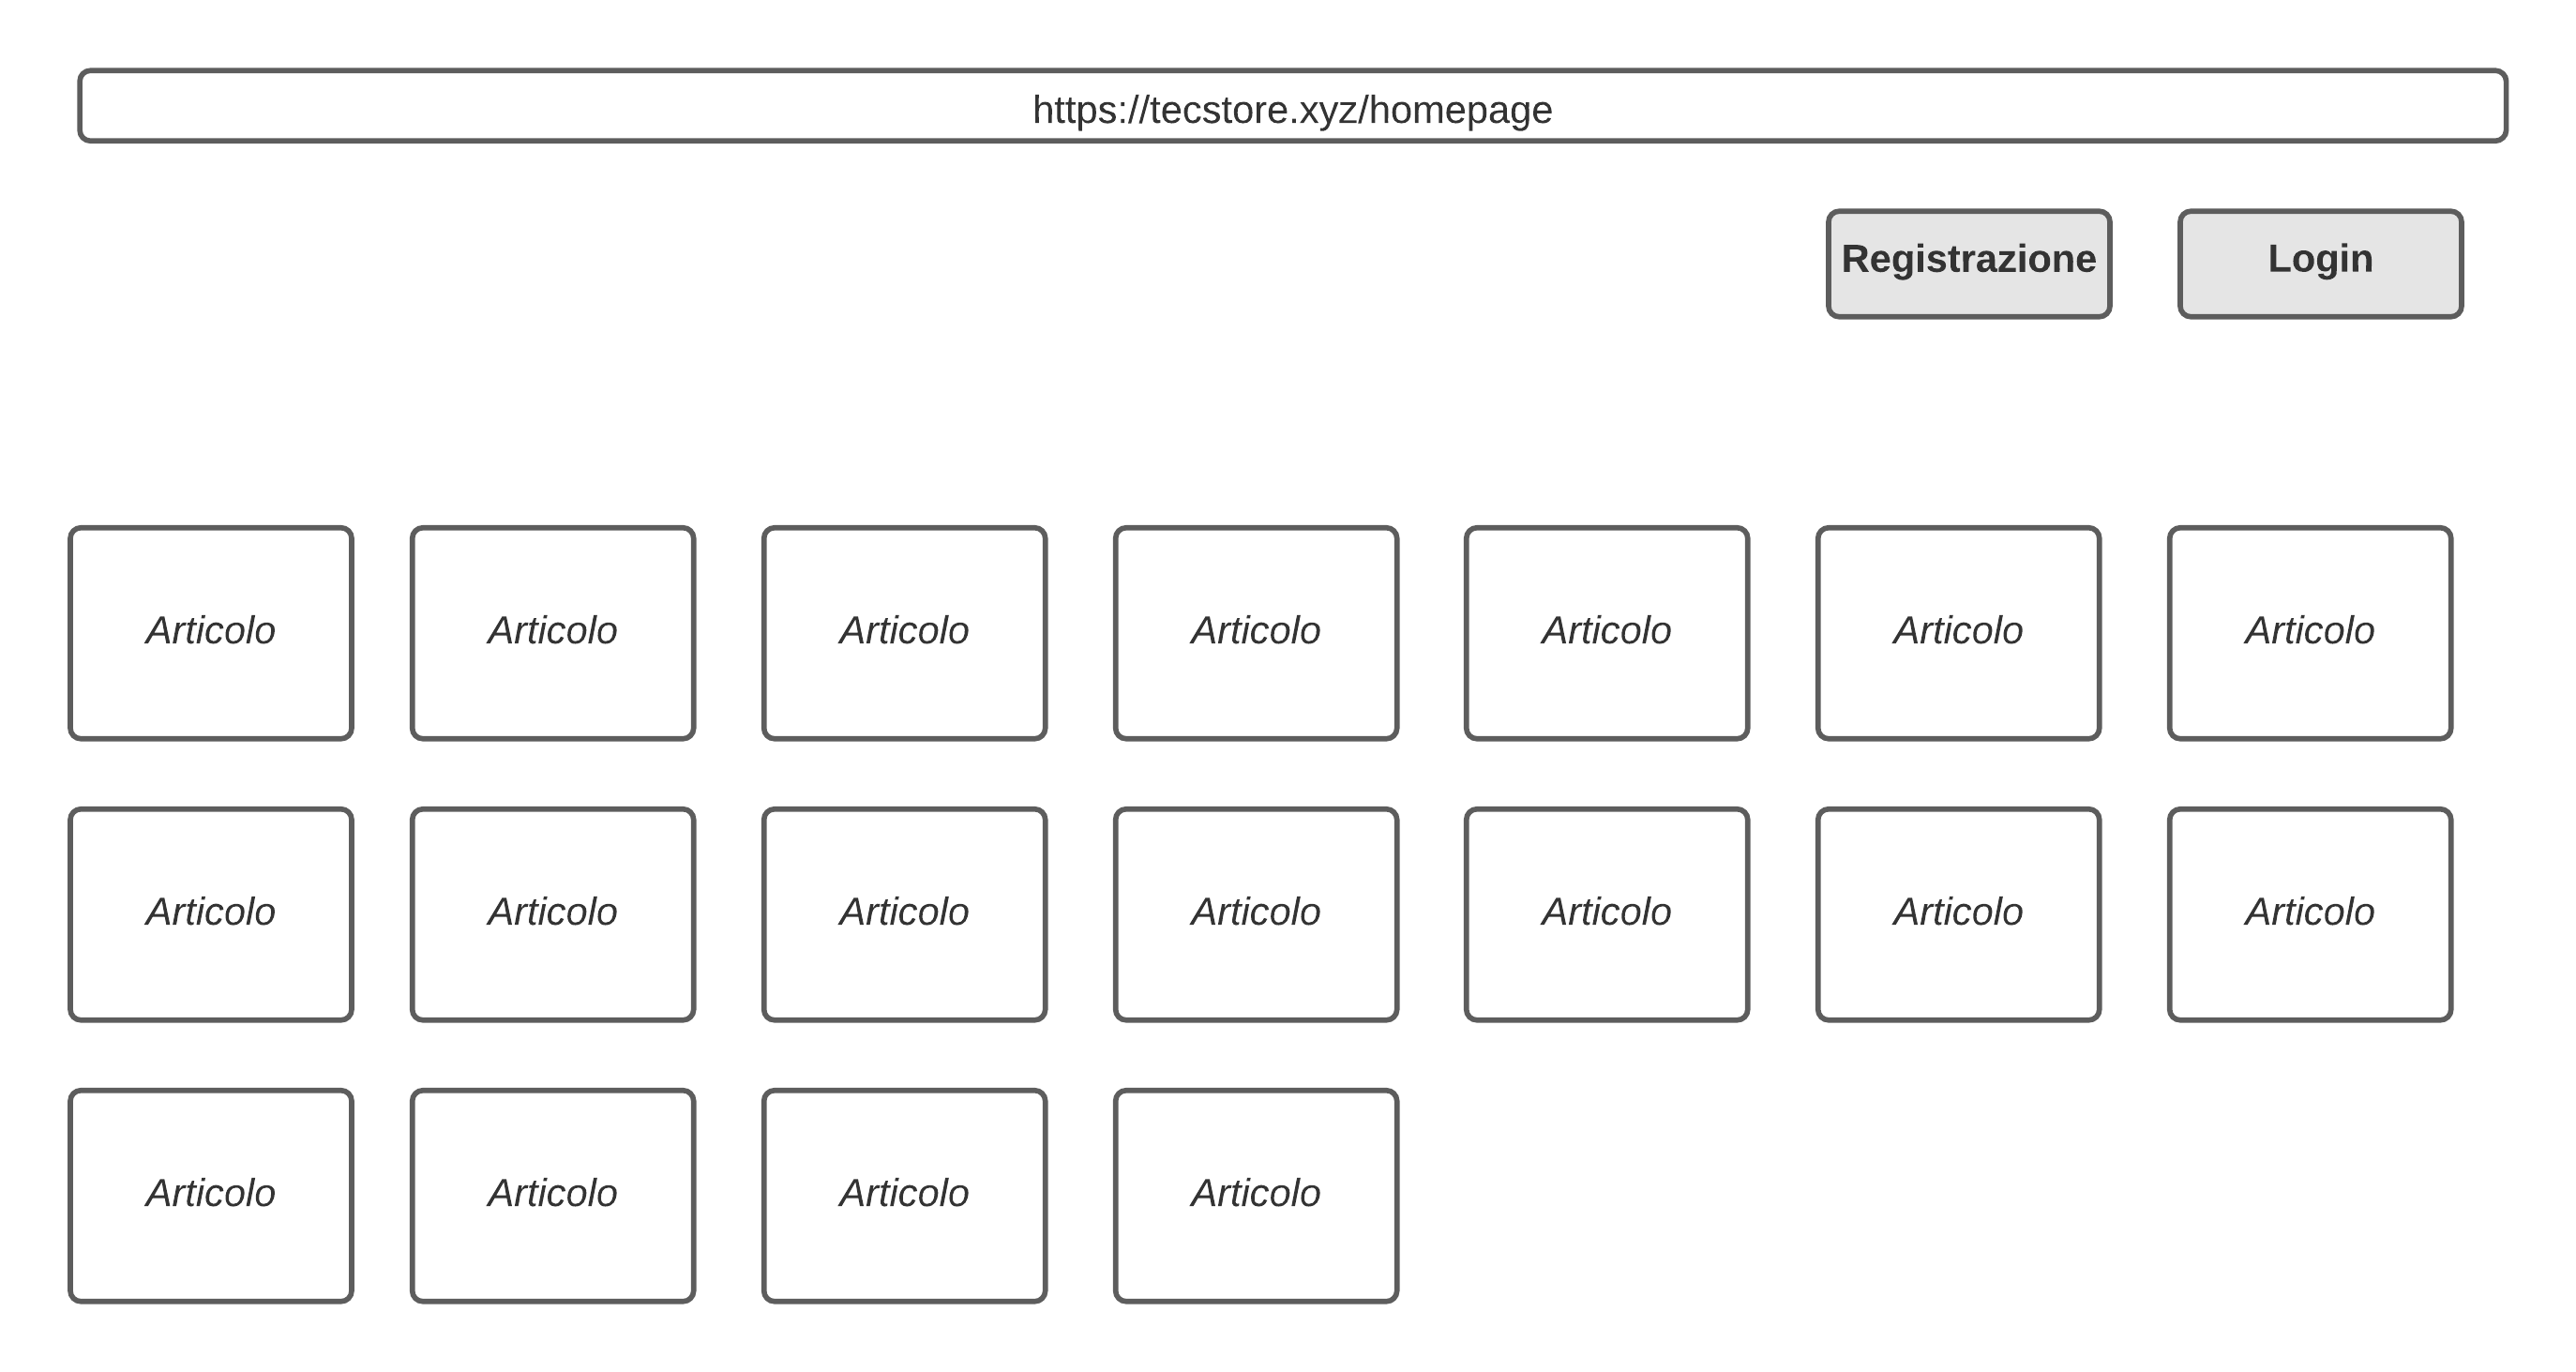
\includegraphics[width=\textwidth]{Mockup/homepage}

\item Inserisce i suoi dati nel form, rispettivamente "alfonsosiciliani@email.tld" e "KDCH5GeWLBBus02fu6W4"

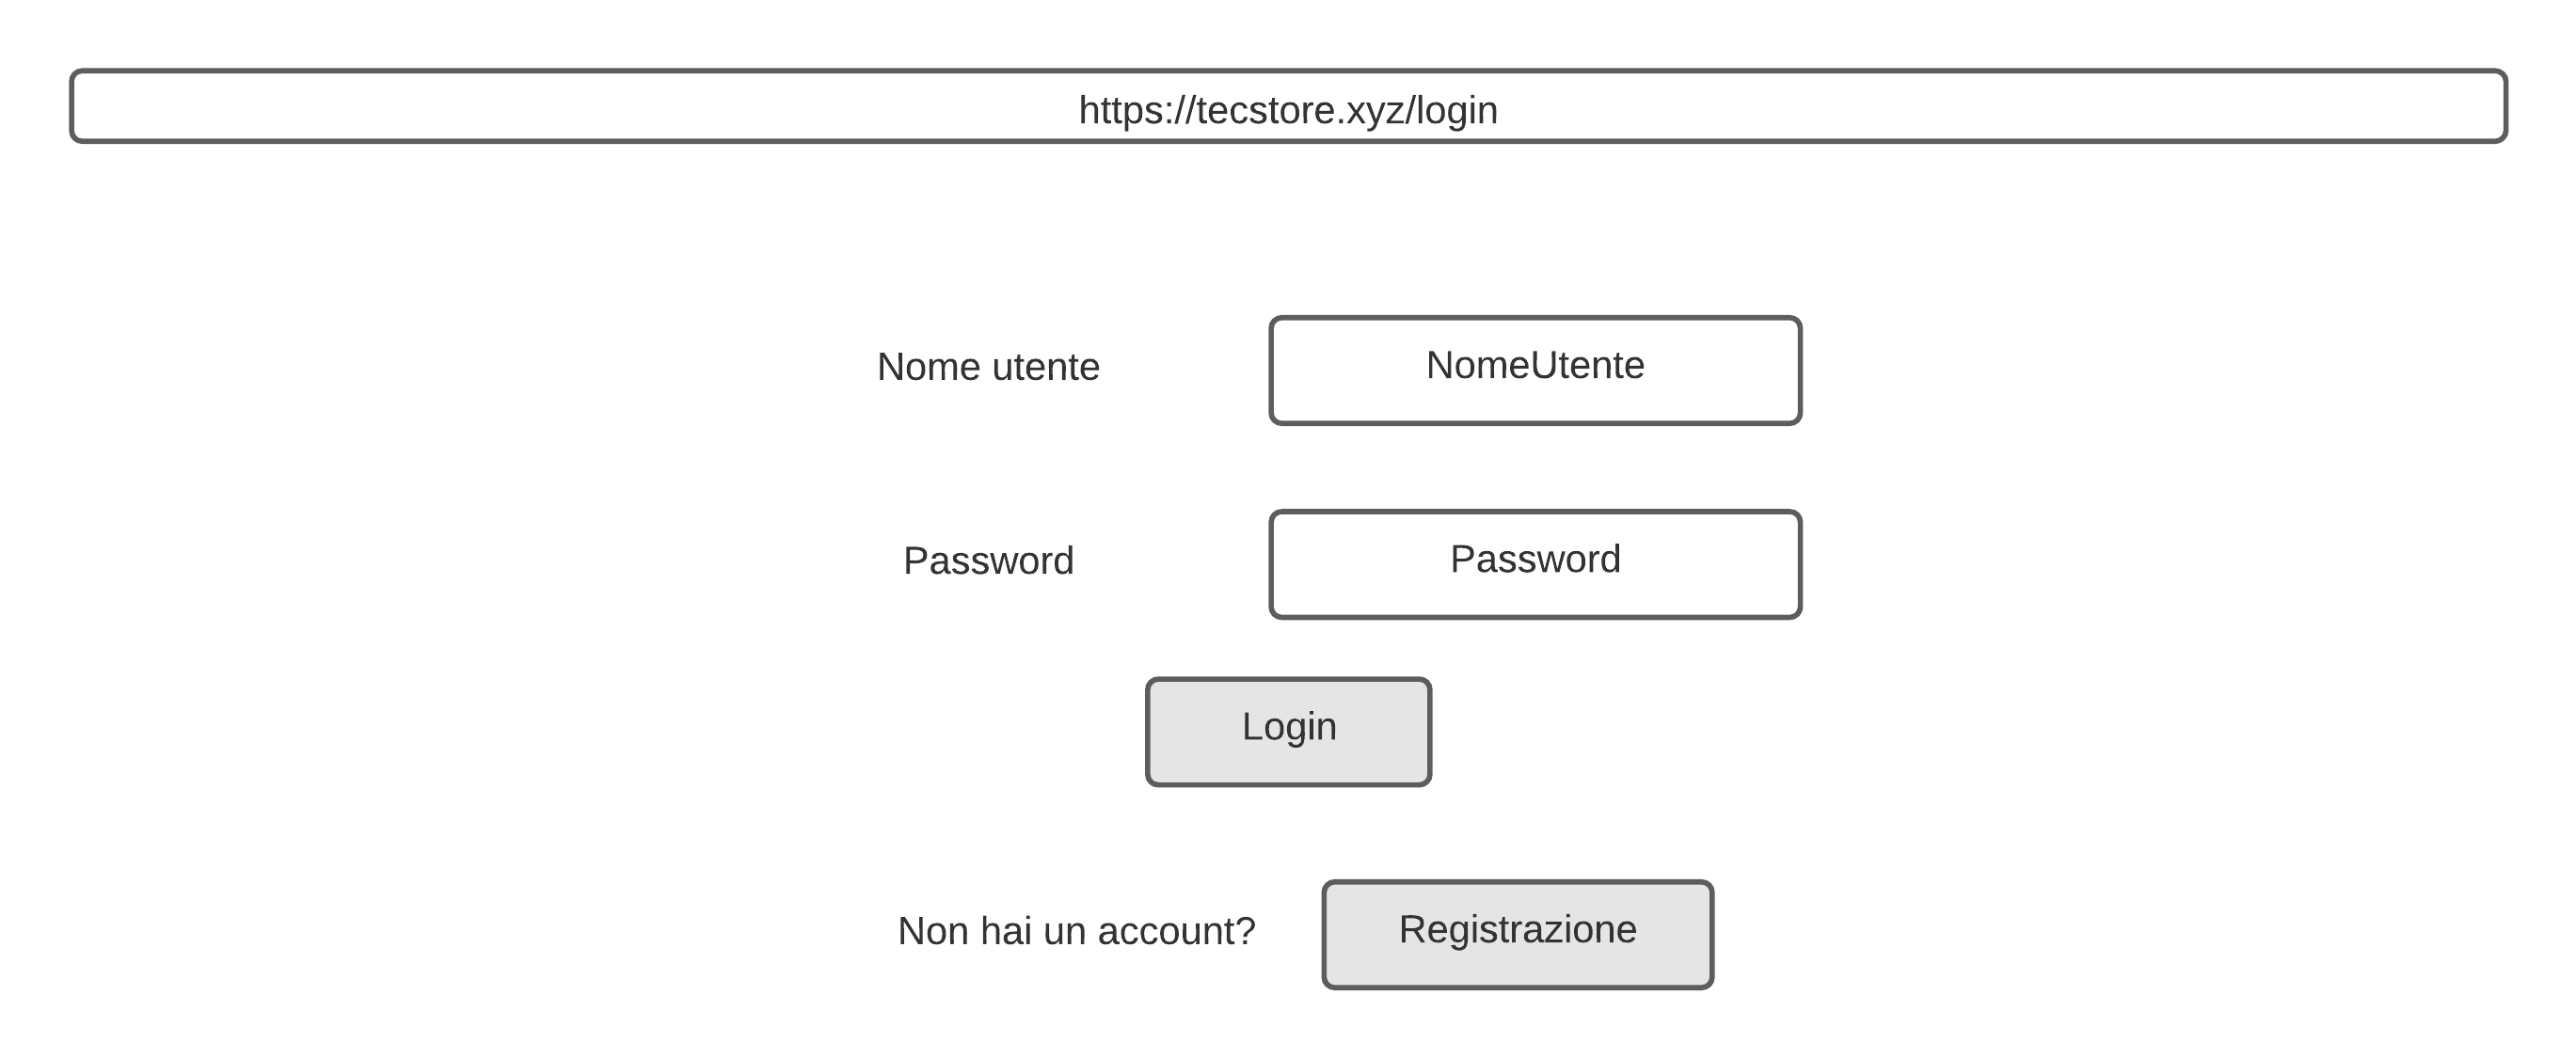
\includegraphics[width=\textwidth]{Mockup/login}

\newpage

\item Viene quindi reindirizzato alla homepage, passa il mouse sul suo nome e clicka sul link "Vendi su TecStore".

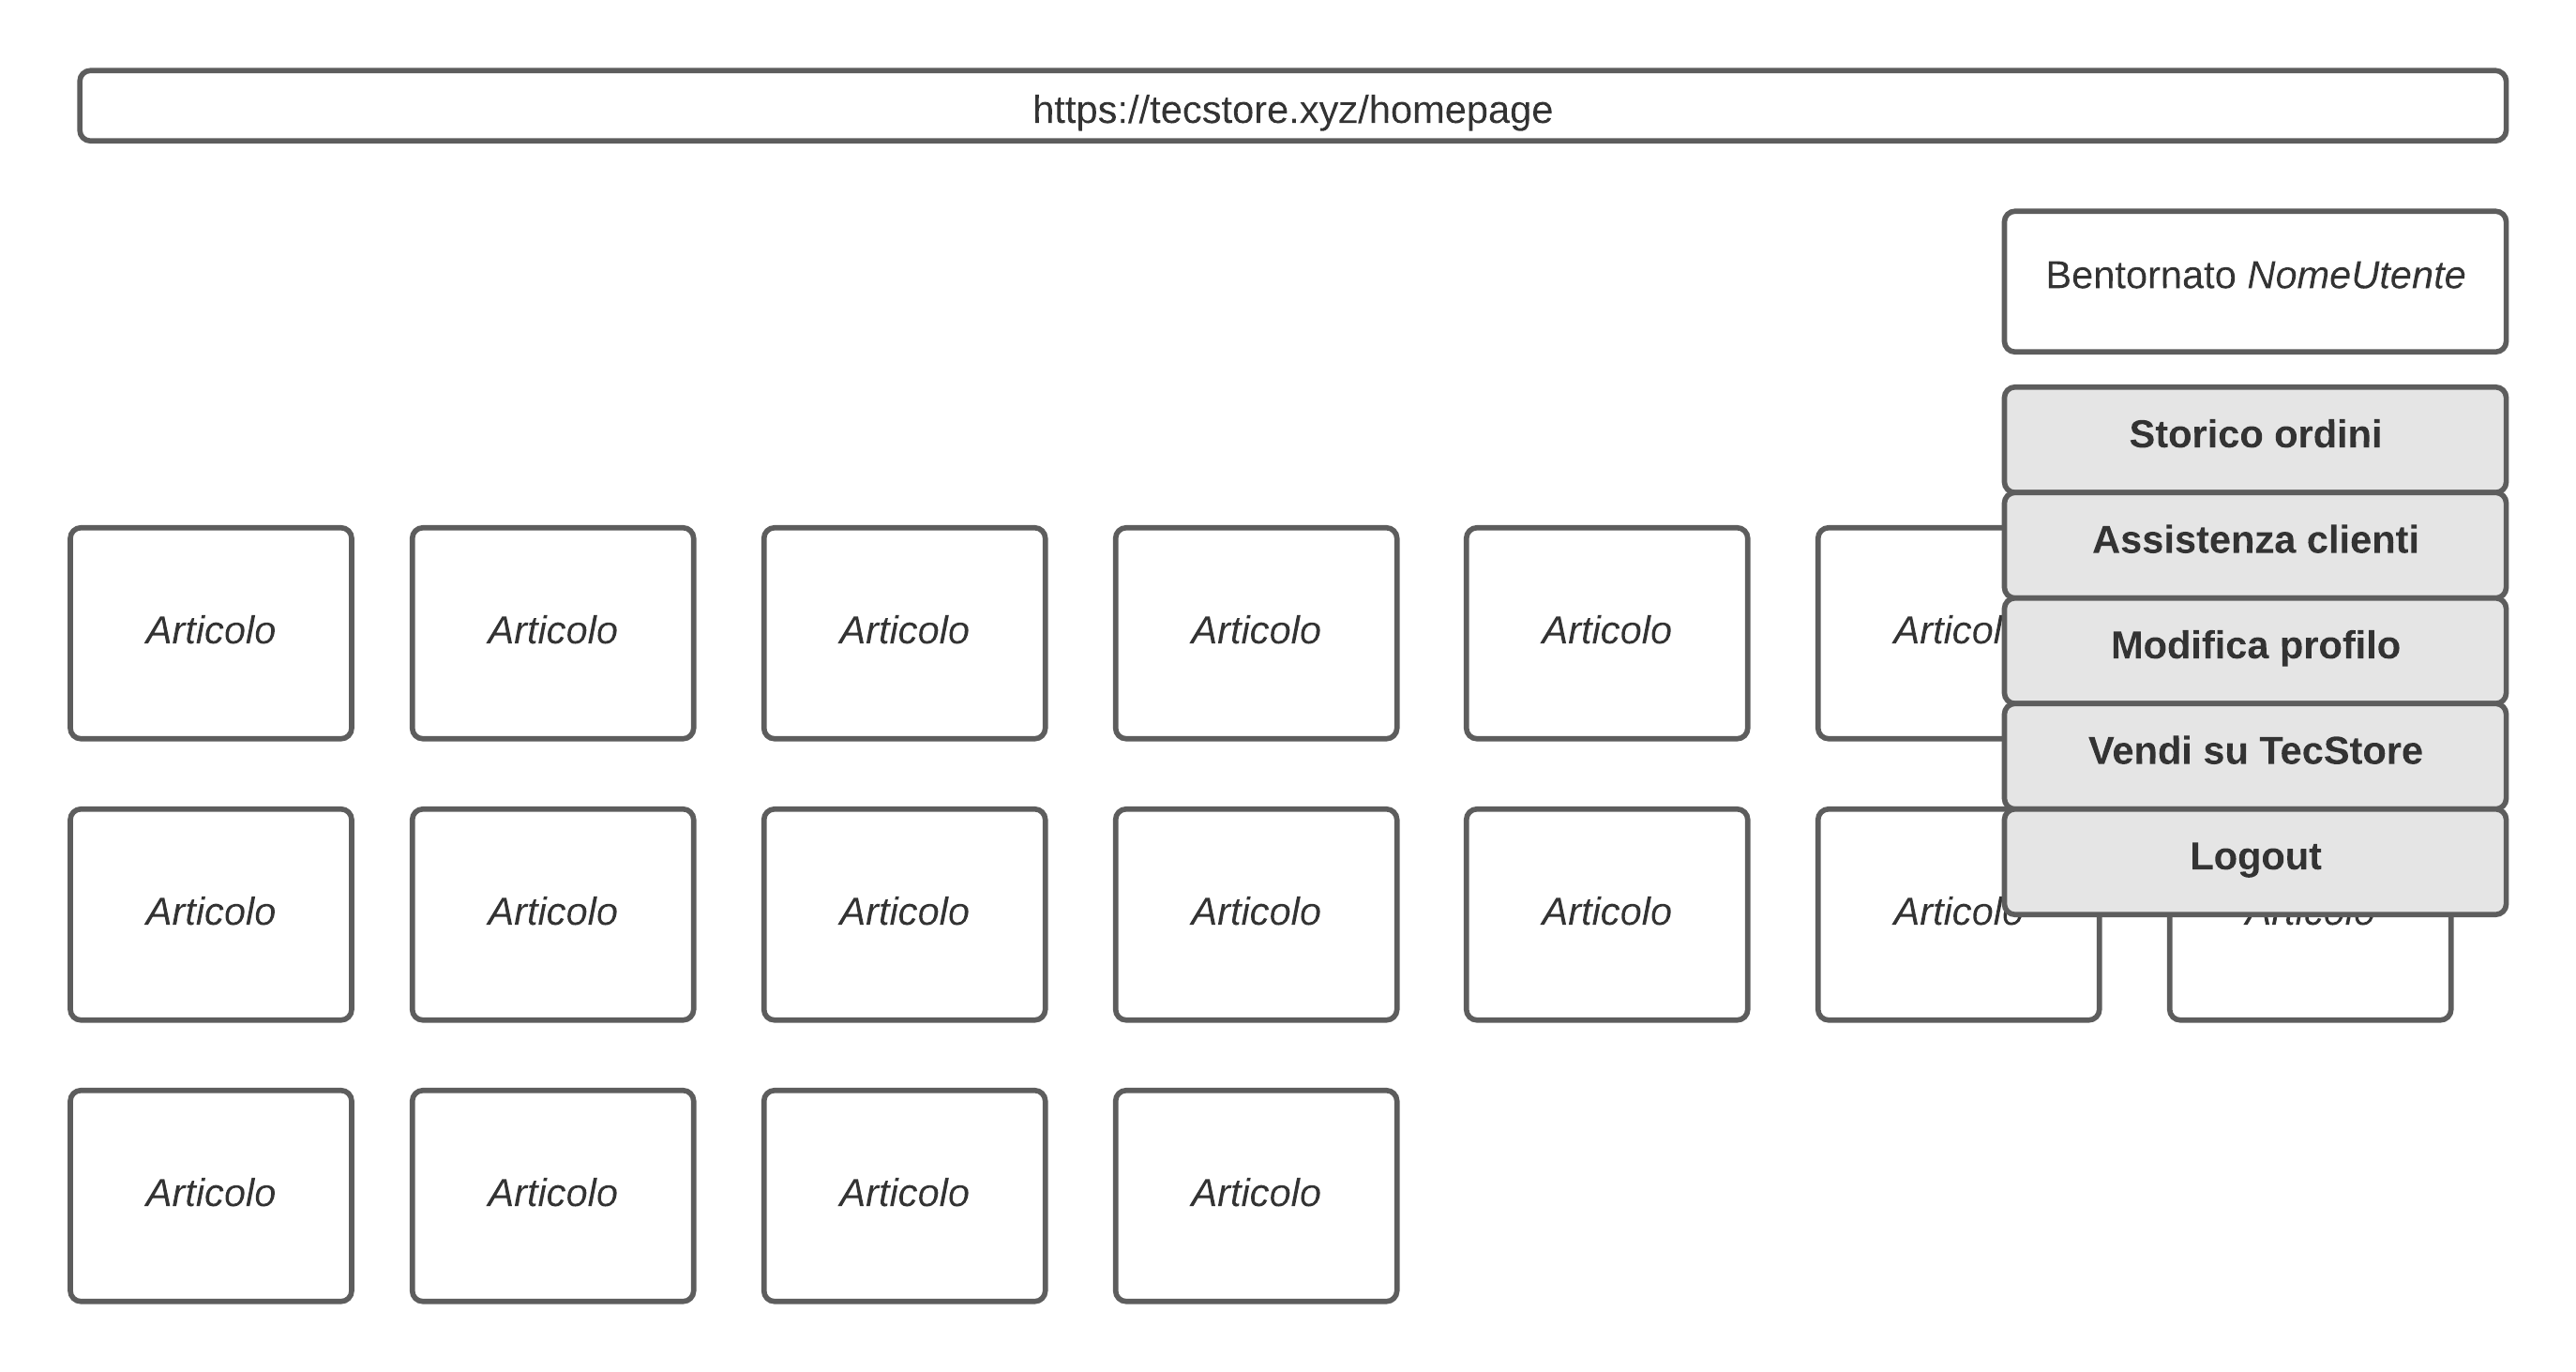
\includegraphics[width=\textwidth]{Mockup/homepage_login}

\item Viene reindirizzato ad una pagina contenente il form per i dati dell'articolo e inserisce, in ordine, "Monitor AOC 22B2H", "Monitor 21.5'' 1080p 75Hz, VGA, HDMI Nero", "8" e "122.25€ e carica alcune foto del dispositivo.

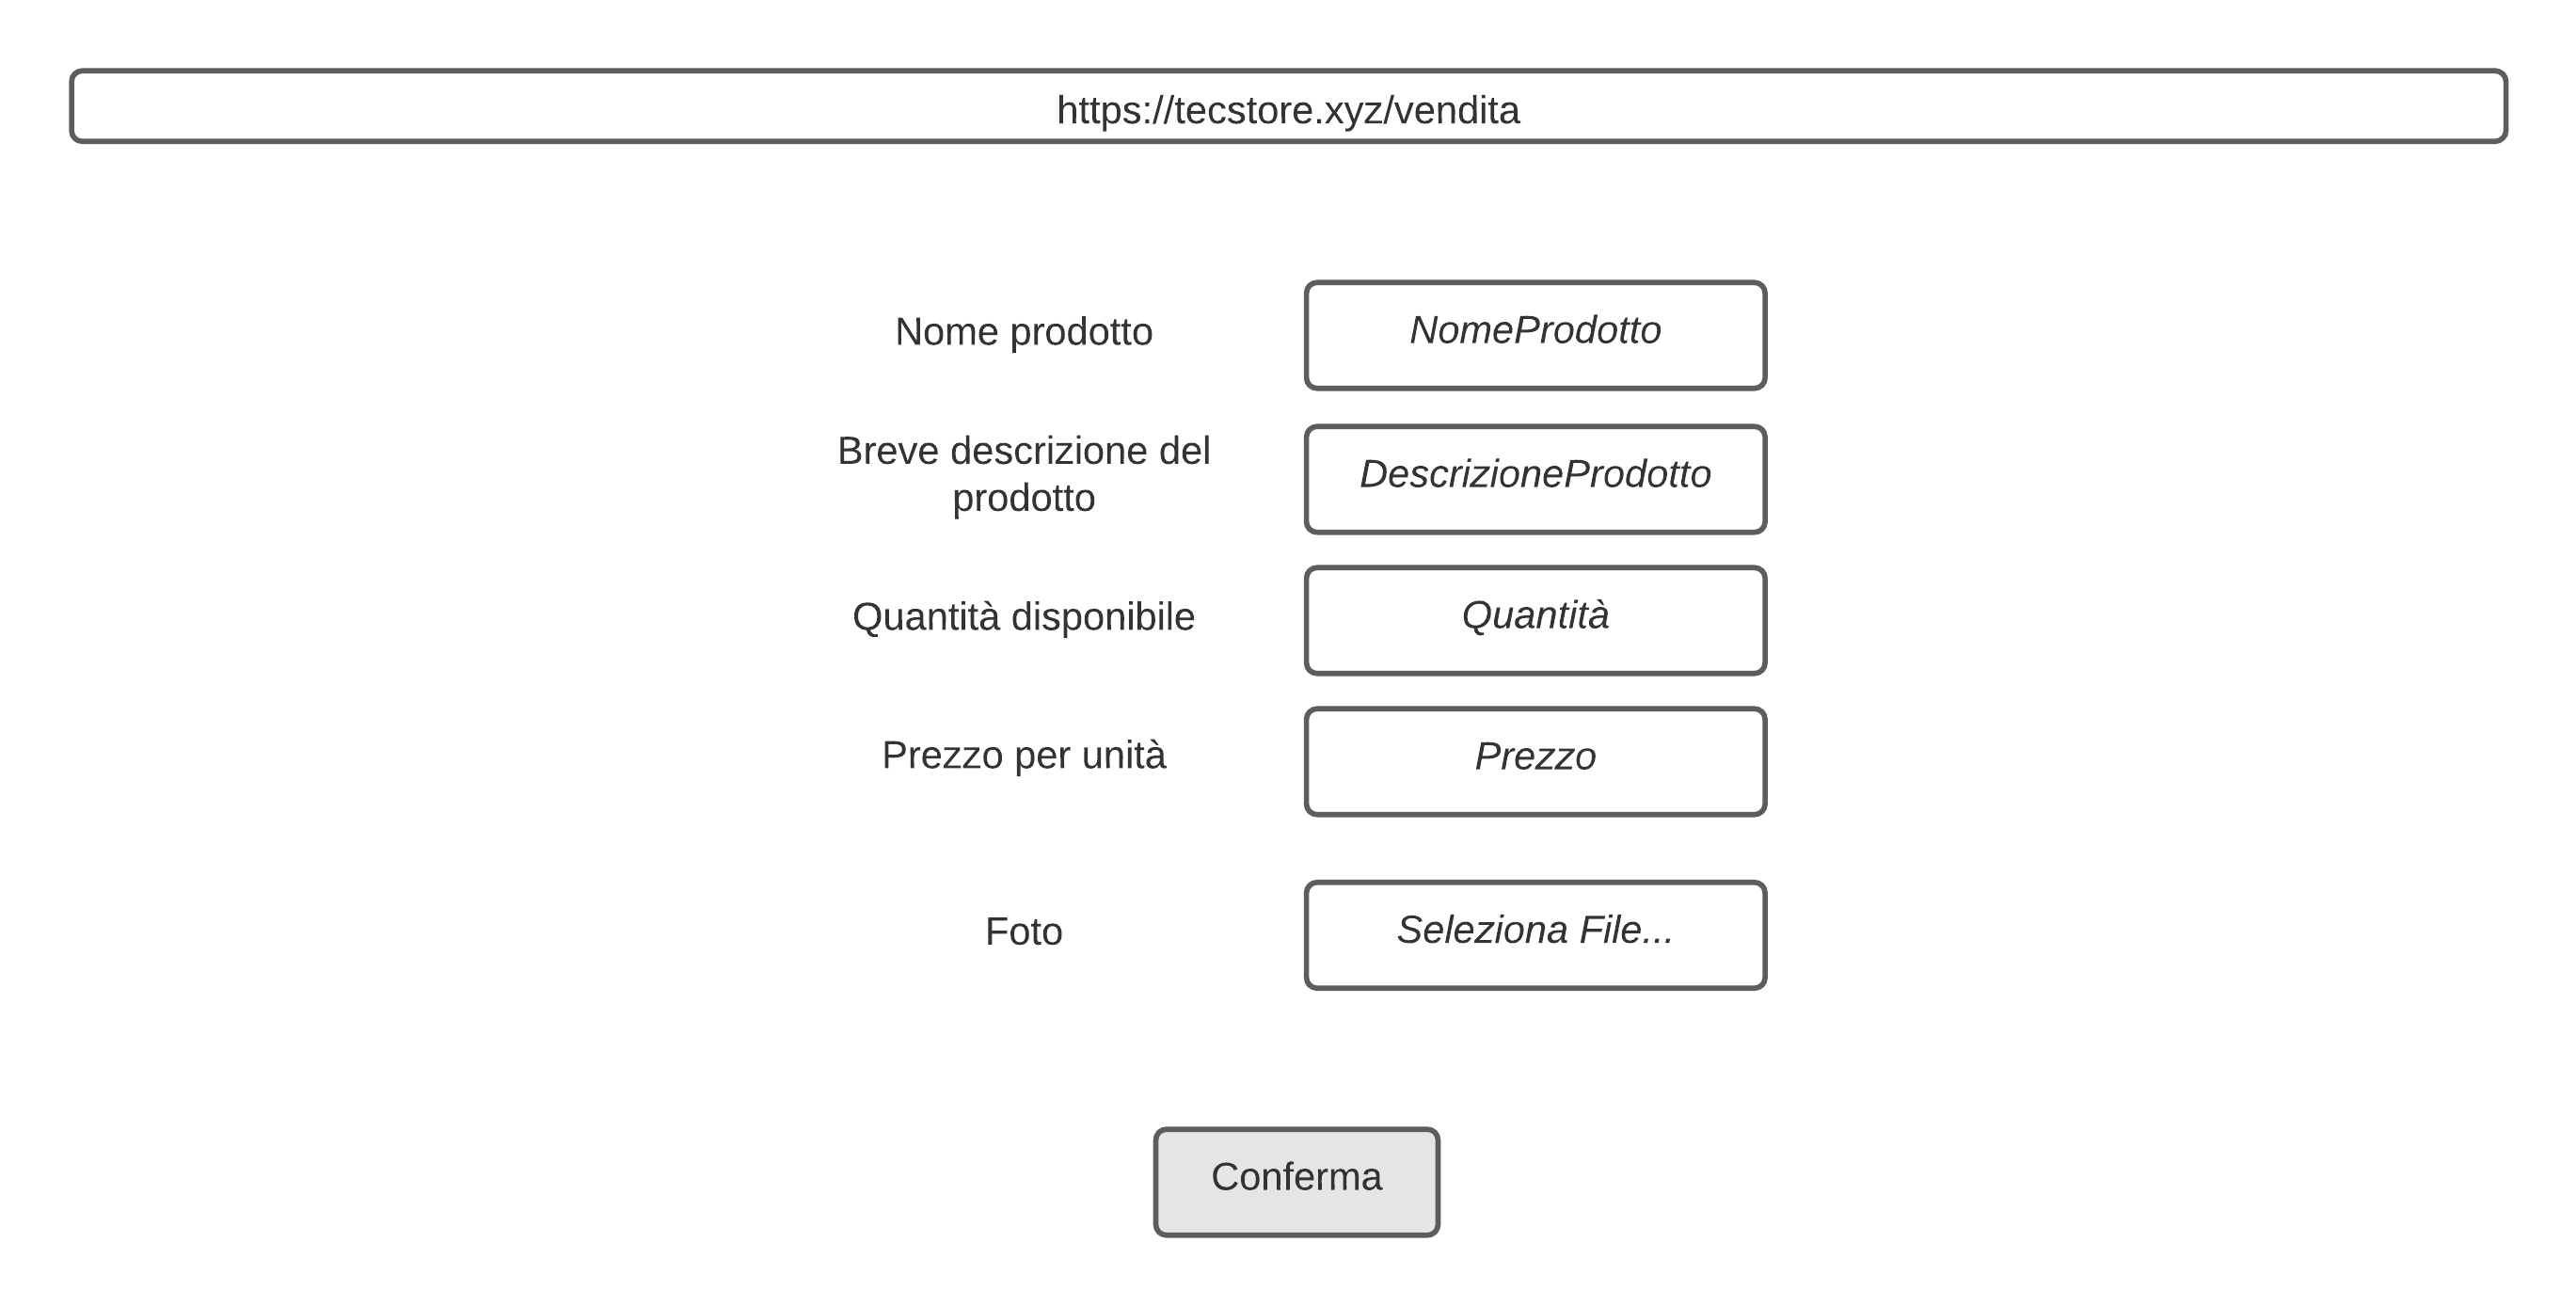
\includegraphics[width=\textwidth]{Mockup/vendita}

\newpage
\item Pochi istanti dopo, un sistema automatico effettua un controllo sommario sul contenuto dell'inserzione e, dato che non contiene profanità o altri contenuti indesiderati, Silvana riceve una notifica nella sua \textit{dashboard}, richiedendo una conferma manuale all'inserimento dell'ordine nel catalogo.

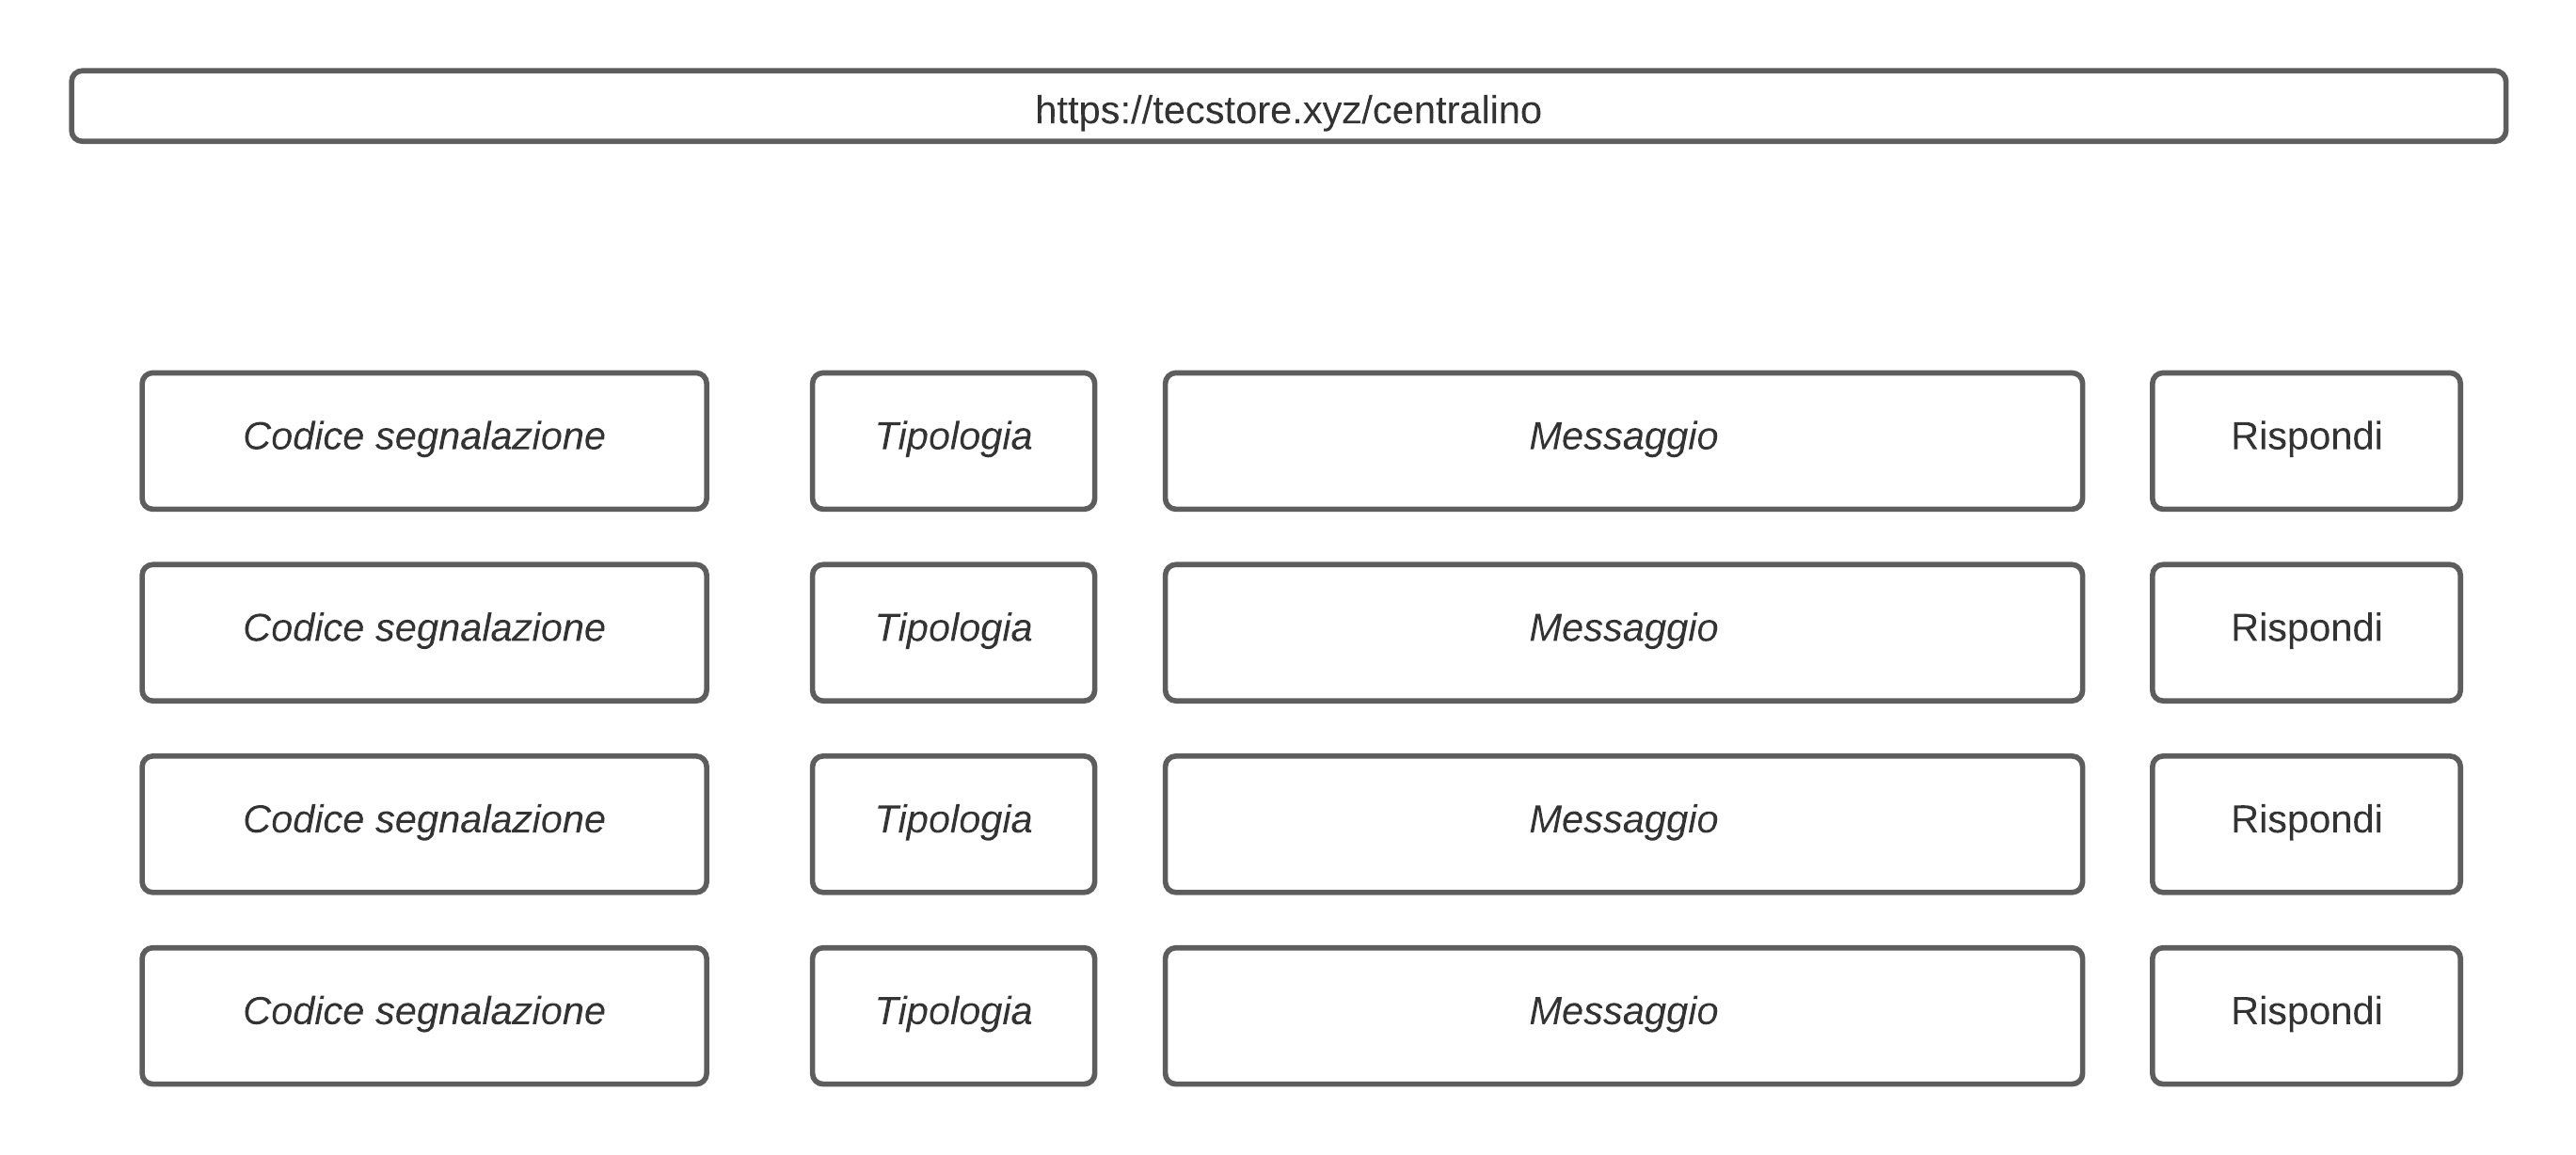
\includegraphics[width=\textwidth]{Mockup/centralino}

\item Dopo aver effettuato delle ulteriori verifiche, Silvana decide di accettare l'inserzione di Alfonso, che apparirà a tutti gli altri utenti.
\end{enumerate}

\newpage

\subsubsection{Il responsabile del personale ha assunto un nuovo centralinista}
\textbf{Attori:} Carlo Martello, responsabile del personale e Matilde Rossi, centralinista \\

\noindent
\textbf{Flusso di eventi:}
\begin{enumerate}
\item Dopo aver sostenuto un colloquio, Matilde è stata assunta come nuova centralinista. Carlo ha il compito di registrare l'identità di Matilde nel sistema, in modo che possa lavorare.

\item Carlo effettua dalla homepage fa click sul pulsante "login" e inserisce le credenziali "HR1" e "waU9qGBrTQ3yXk21MZwo"

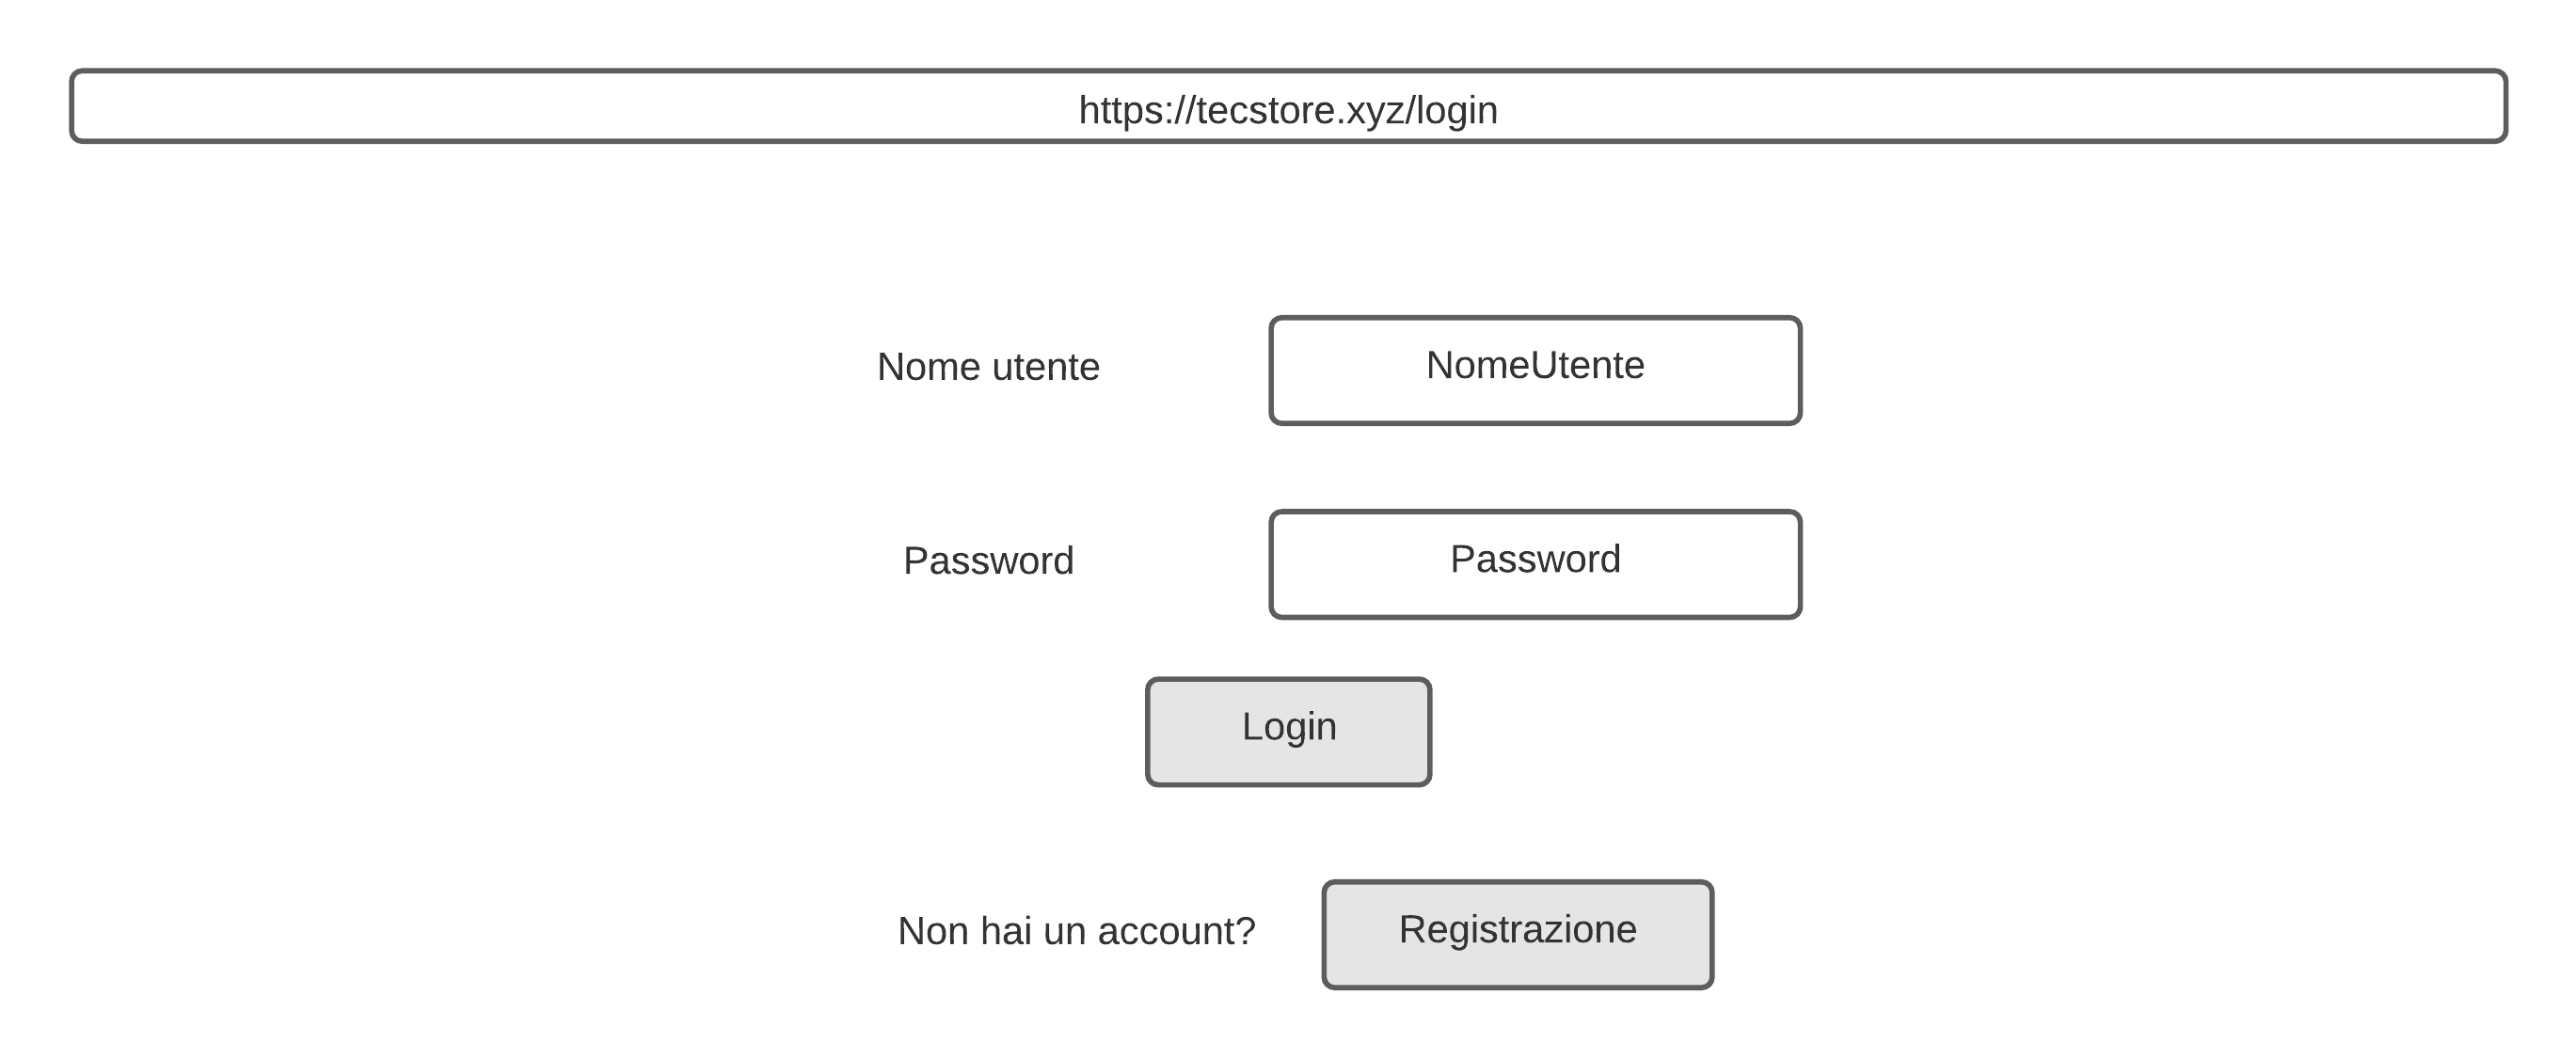
\includegraphics[width=\textwidth]{Mockup/login}

\newpage
\item Viene reindirizzato alla pagina per la gestione del personale, dalla quale fa click sul pulsante per aggiungere un nuovo dipendente

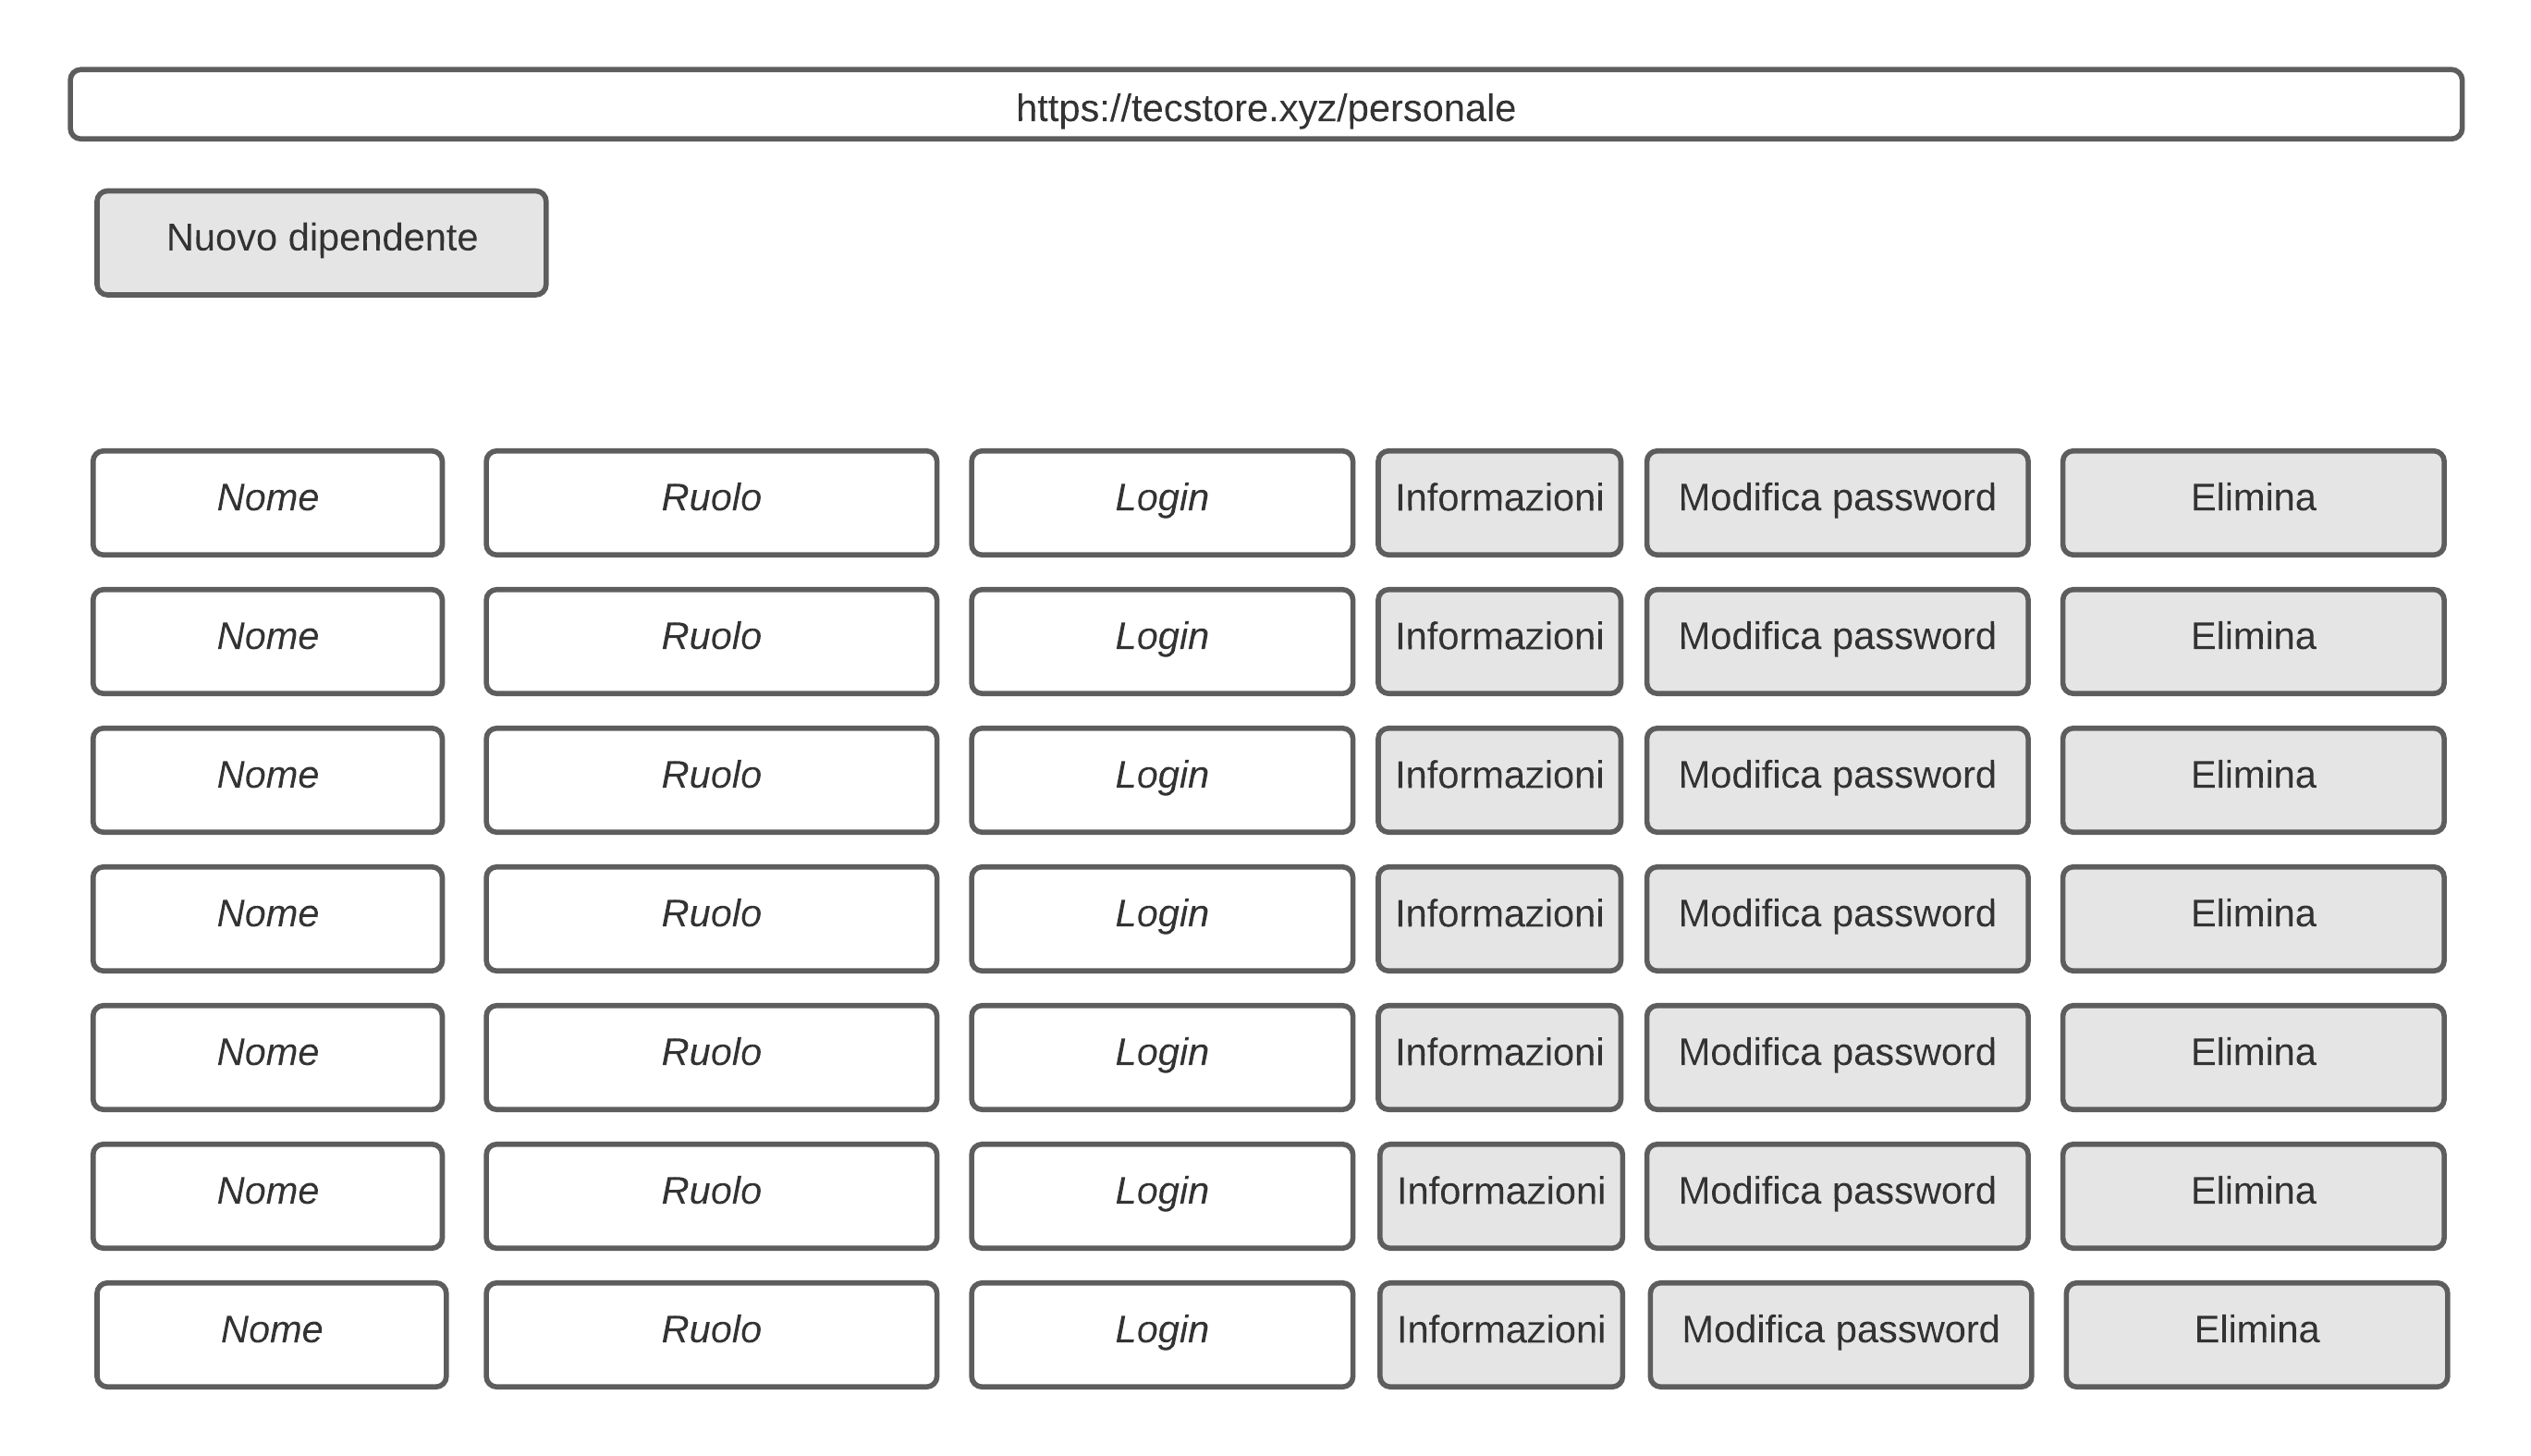
\includegraphics[width=\textwidth]{Mockup/personale}

\item Viene reindirizzato al form per la creazione di un nuovo dipendente, in cui inserisce, in ordine, "Matilde", "Rossi", "21/04/1987", "Roma", "RSSMLD87D61H501M", "Roma", "Via Torino, 1", "IT18T0300203280984179265554", "Centralino" e fa click su conferma.

\begin{center}
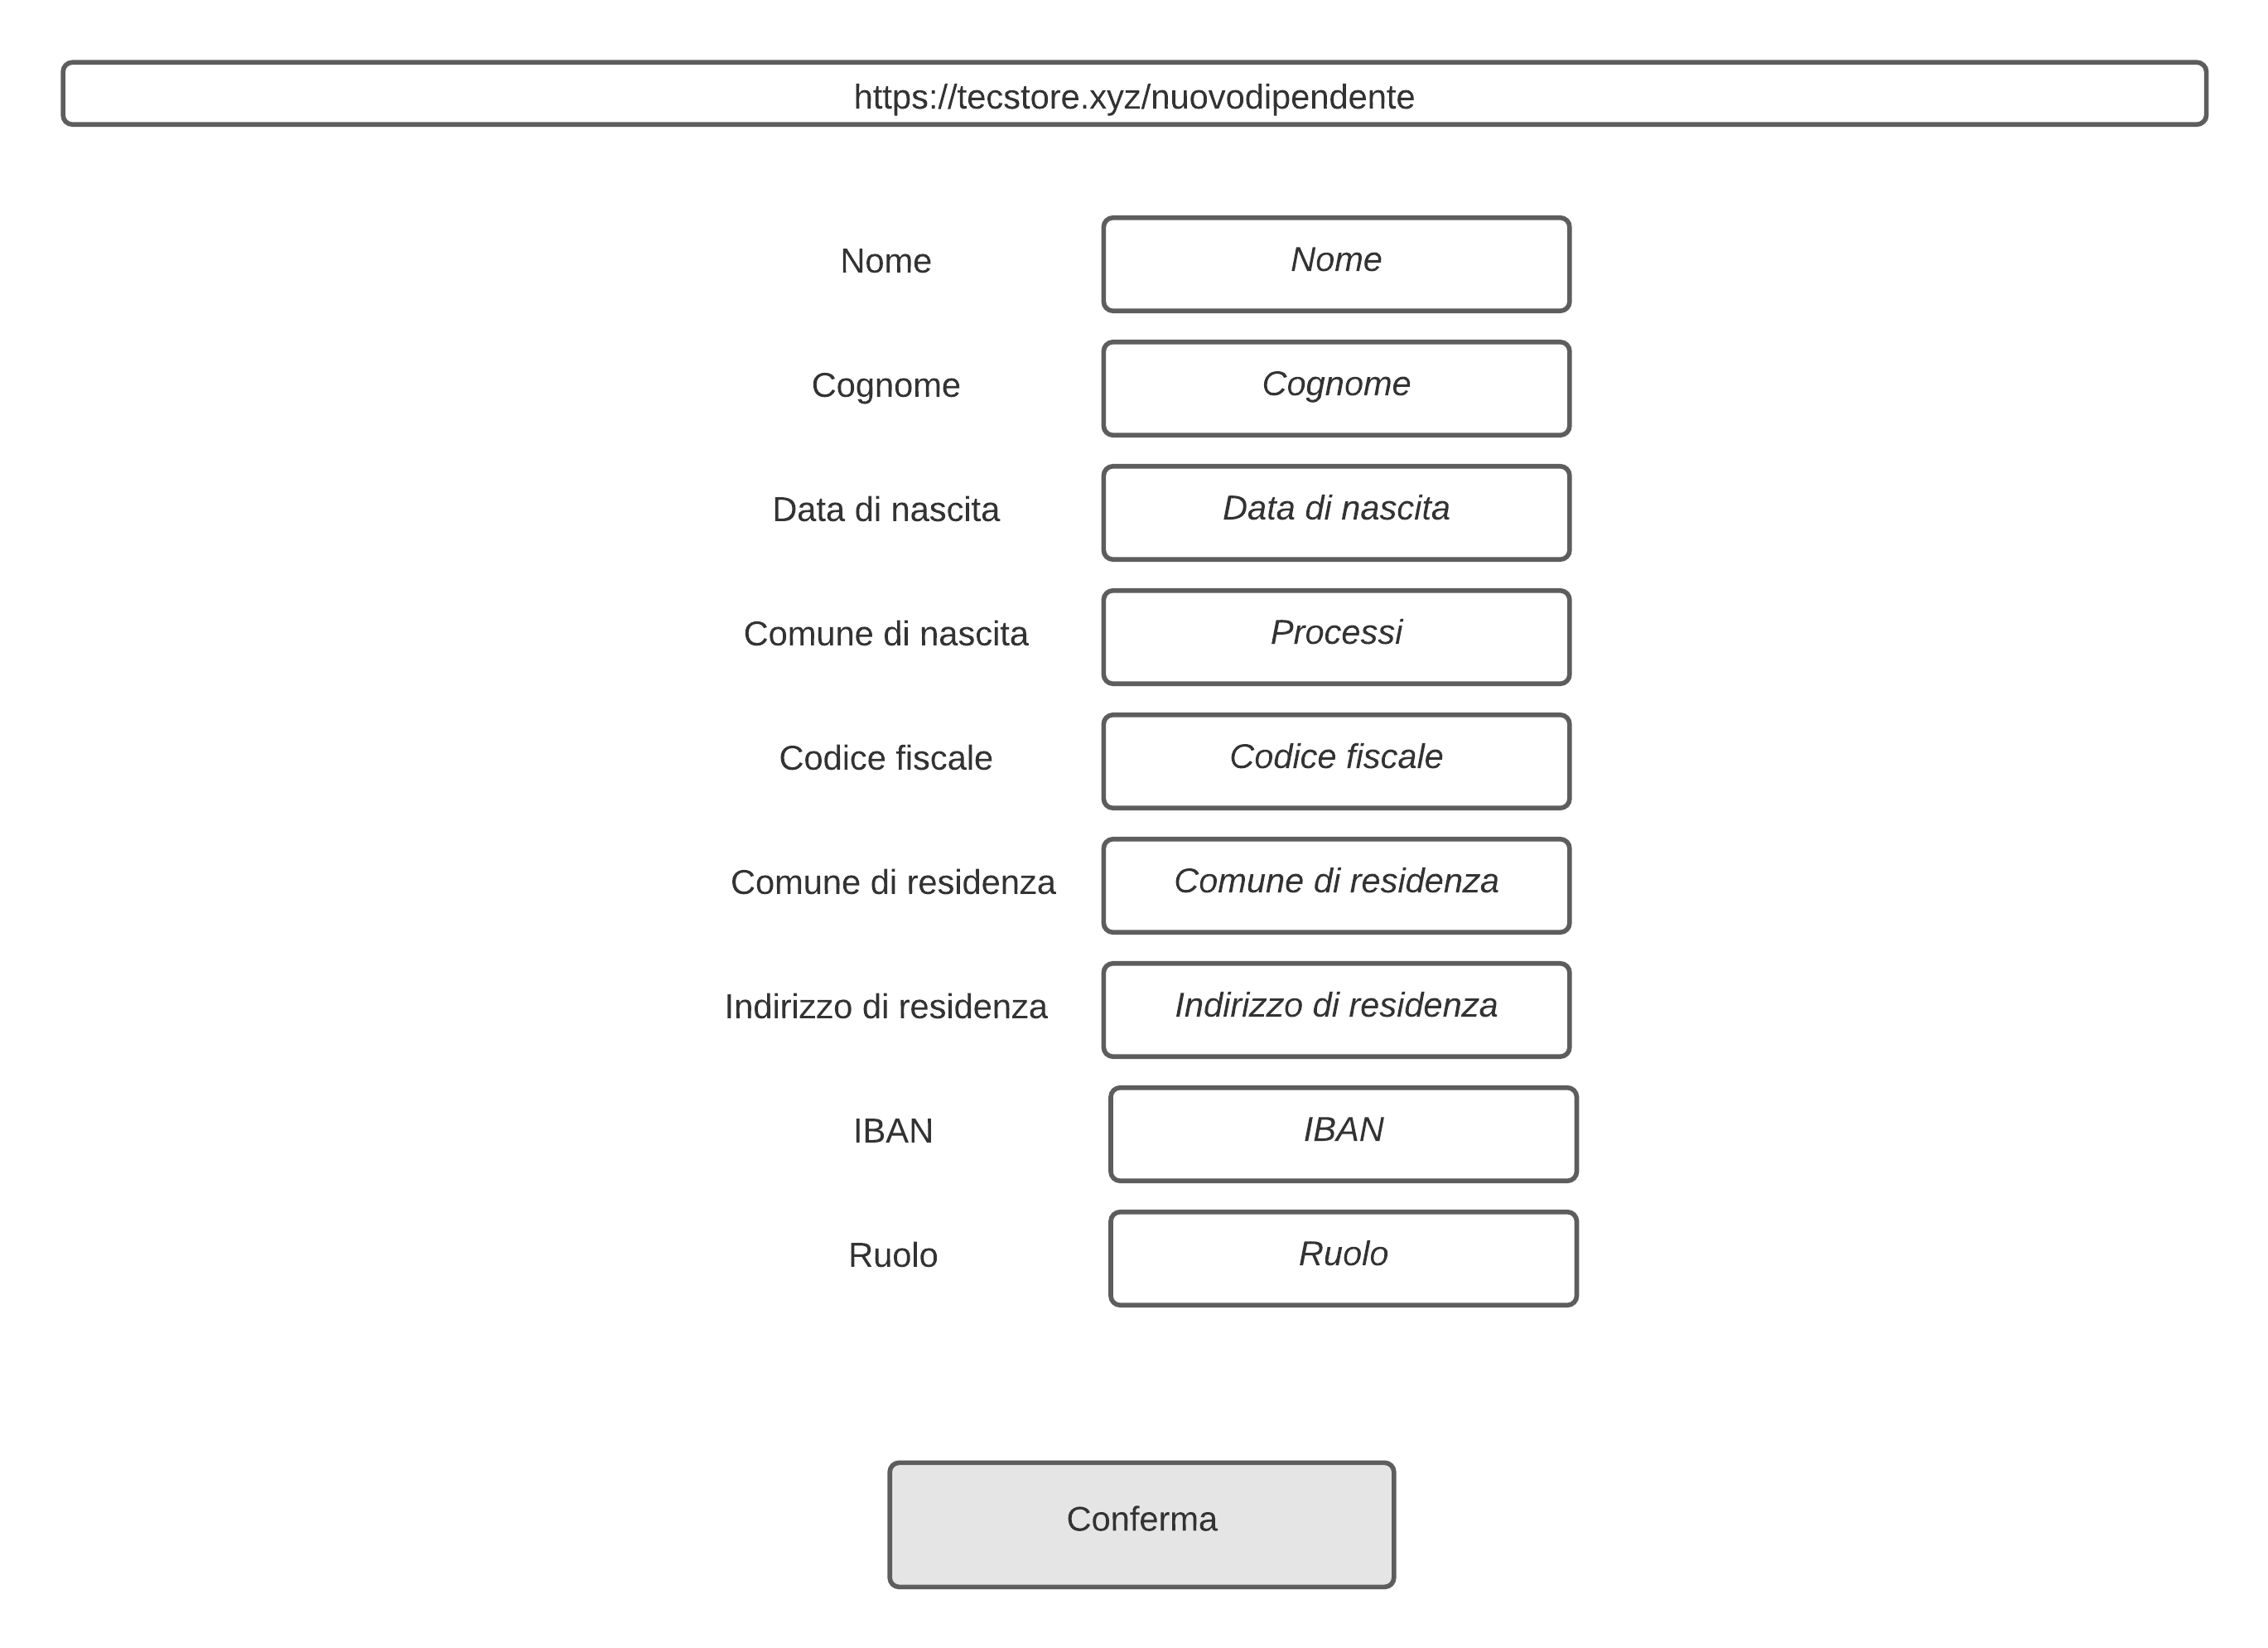
\includegraphics[height=250px]{Mockup/nuovodipendente}
\end{center}

\newpage
\item Viene mostrata una pagina contenente le informazioni di accesso per Matilde generate dal sistema, con un avviso di stampare i dati e conservarli in un luogo sicuro.

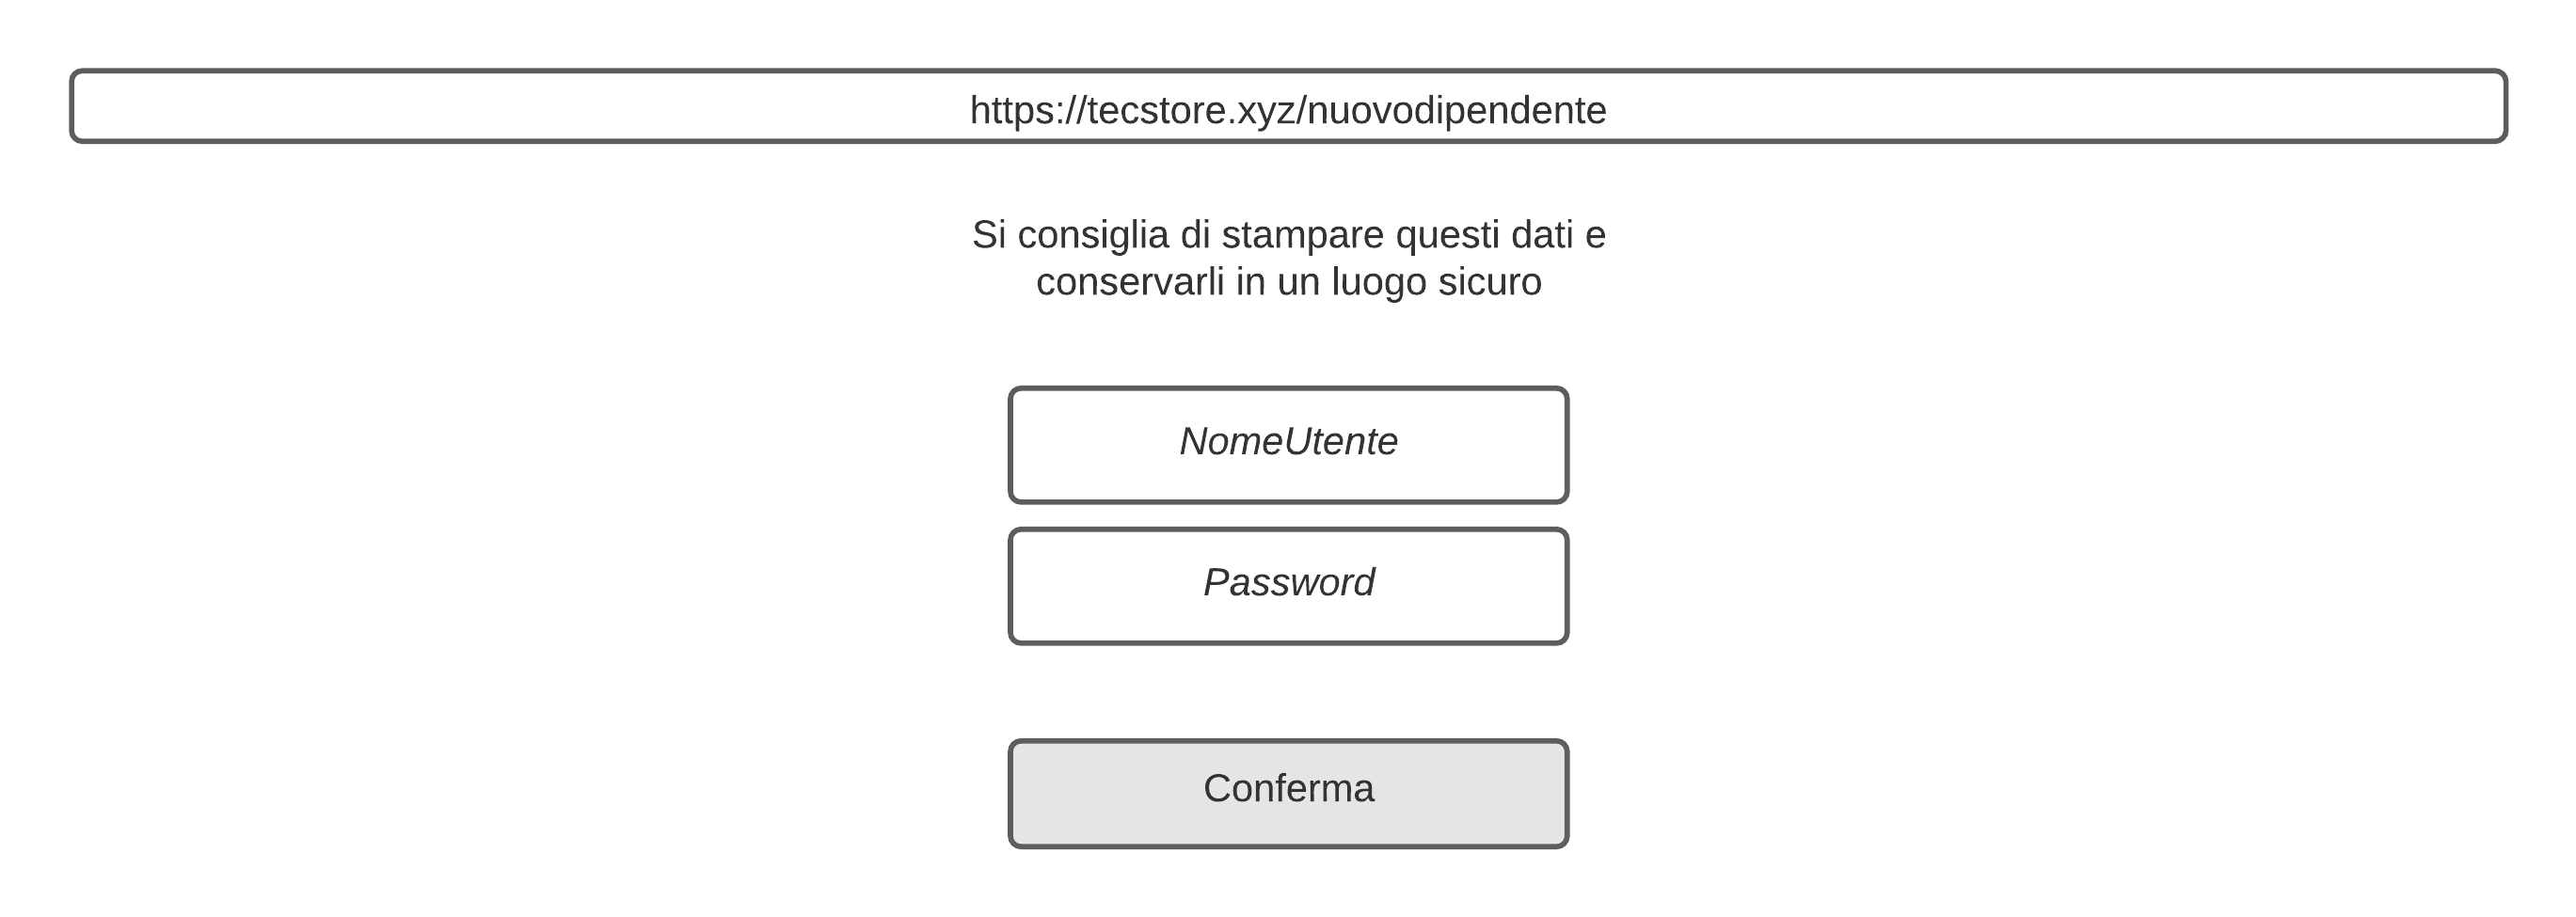
\includegraphics[width=\textwidth]{Mockup/nuovodipendente2}

\item Il lunedì successivo Matilde inizia il suo primo giorno di lavoro e utilizza le credenziali ricevute per accedere alla pagina del centralino.

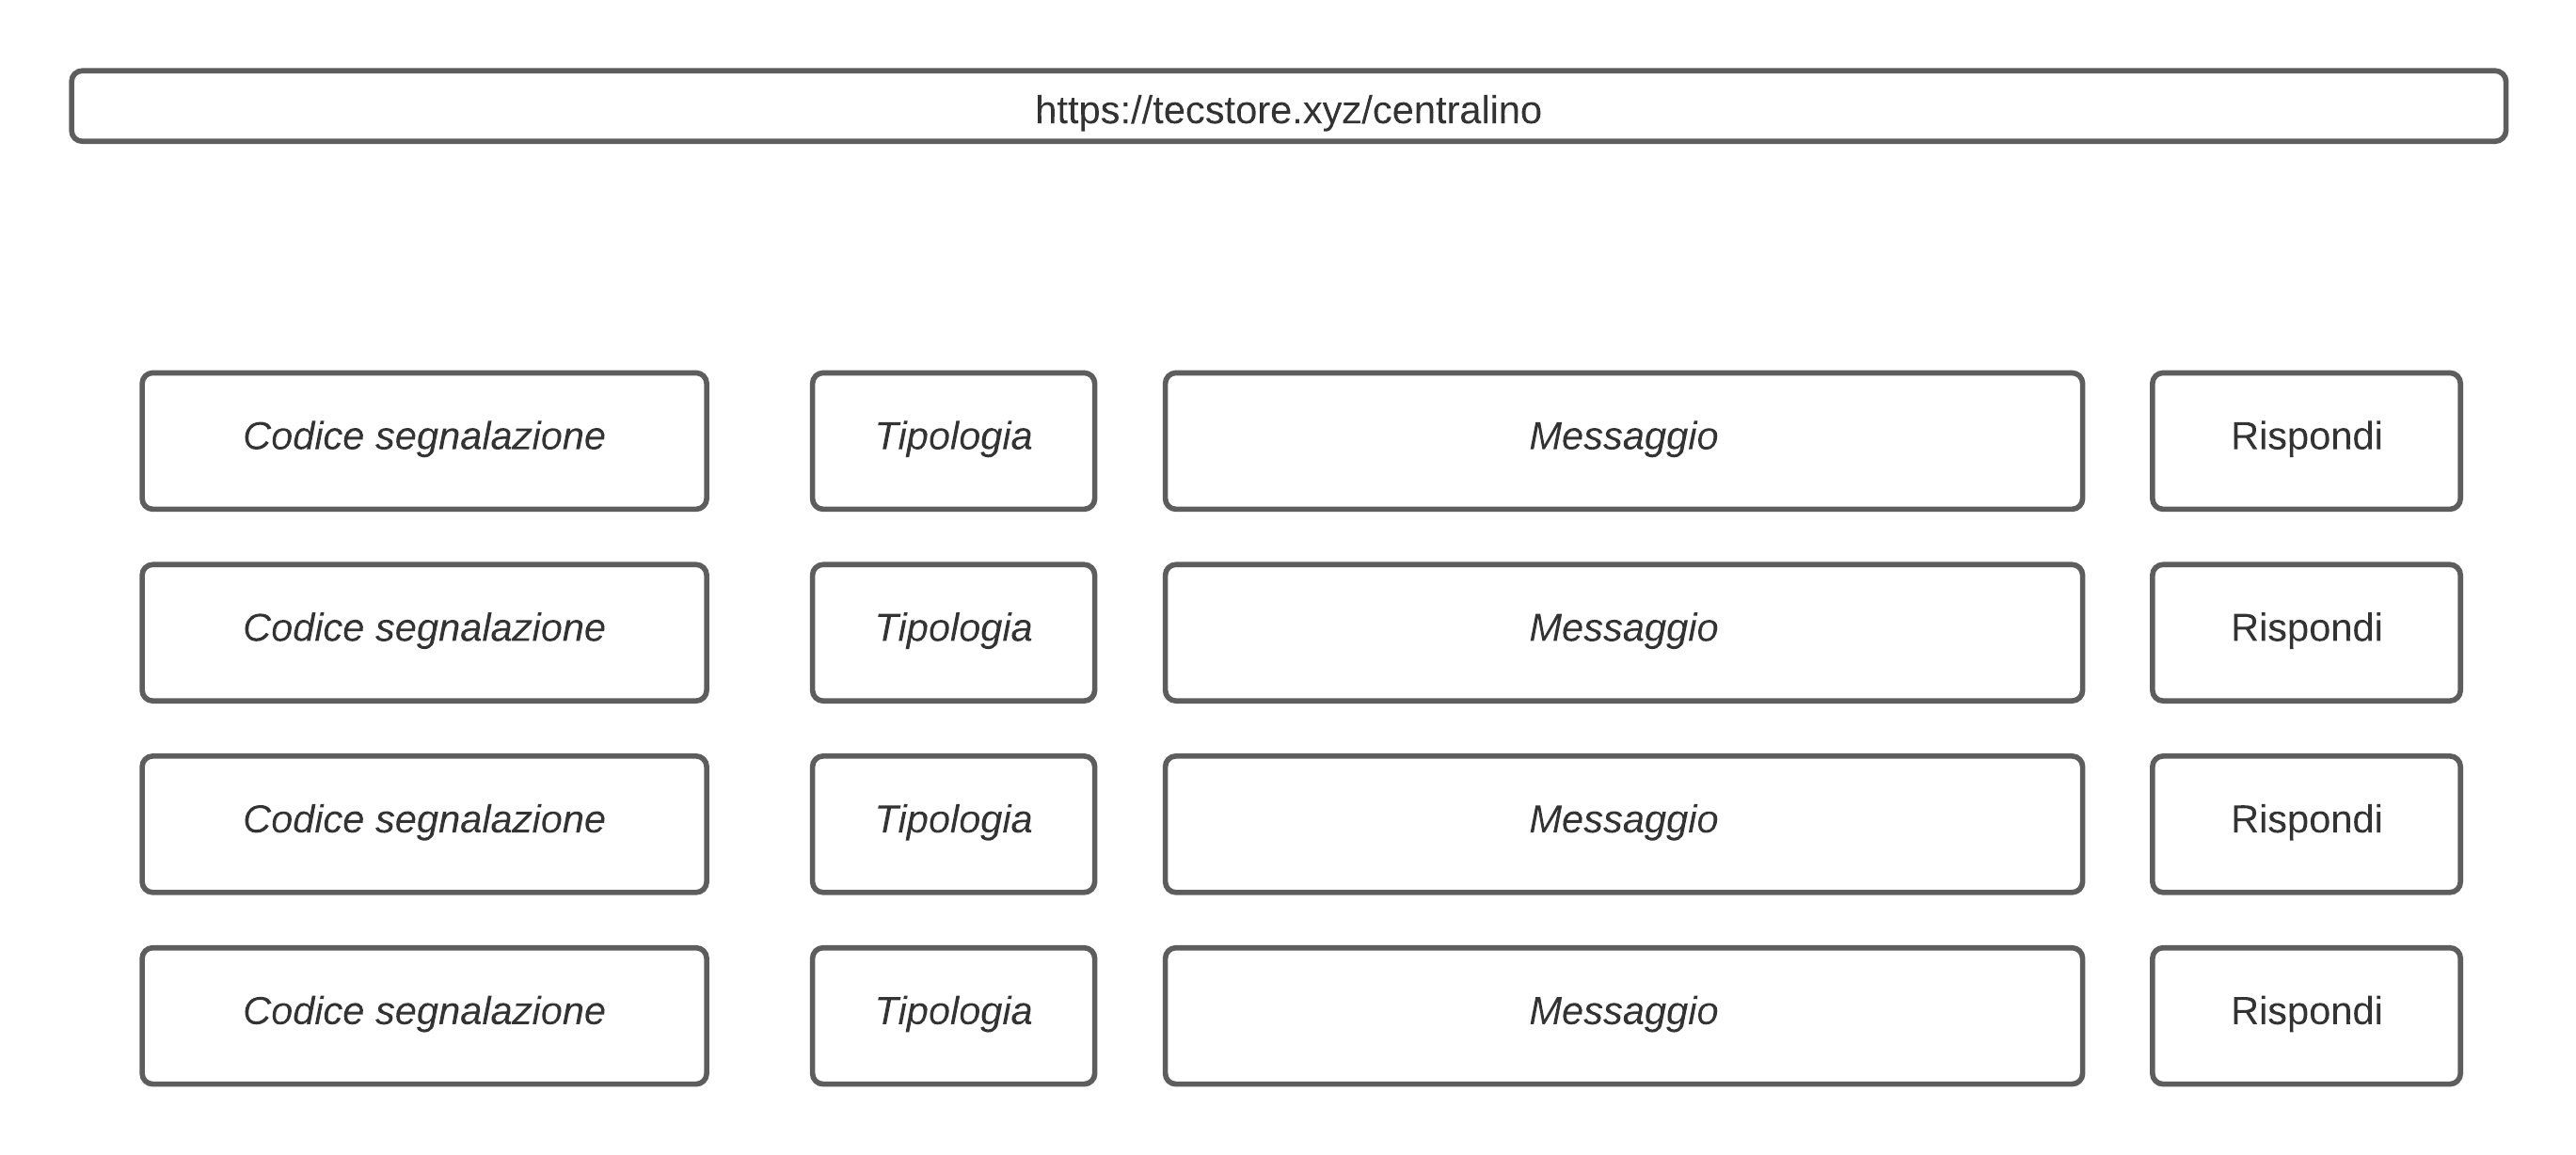
\includegraphics[width=\textwidth]{Mockup/centralino}

\end{enumerate}


\newpage
\section{Use case}
\subsection{Clienti}
\subsubsection{Registrazione di un cliente}
\label{UC:1}
\begin{tabular}{|>{\columncolor[gray]{0.8}}c|p{12cm}|}
\hline
\textbf{ID} & UC1 Registrazione \\
\hline
\textbf{Nome} & Registrazione di un nuovo cliente. \\
\hline
\textbf{Partecipanti} & Utente non registrato \\
\hline
\textbf{Condizione d'ingresso} & Un nuovo cliente visita il sito per la prima volta. \\
\hline
\textbf{Flusso di eventi} &
\begin{minipage}{12cm}
\begin{tabular}{p{5.5cm} p{5.5cm}}
\textbf{Cliente} & \textbf{Sistema} \\
Si collega al sito, nella homepage fa click sul tasto "Registrati" & \\
& Mostra al cliente il form per la registrazione in cui inserire tutti i dati personali, incluso nome, cognome, indirizzo, numero di carta di credito. \\
Inserisce tutti i suoi dati, fa click su "Registrati". & \\
& Se le credenziali sono corrette, invia al cliente una mail di conferma e chiede al cliente di utilizzare il link per confermare l'account. \\
\end{tabular}
\end{minipage} \\

\hline
\textbf{Condizione d'uscita} & Il cliente si registra. \\

\hline
\end{tabular}


\bigskip
\bigskip
\label{UC:1d}

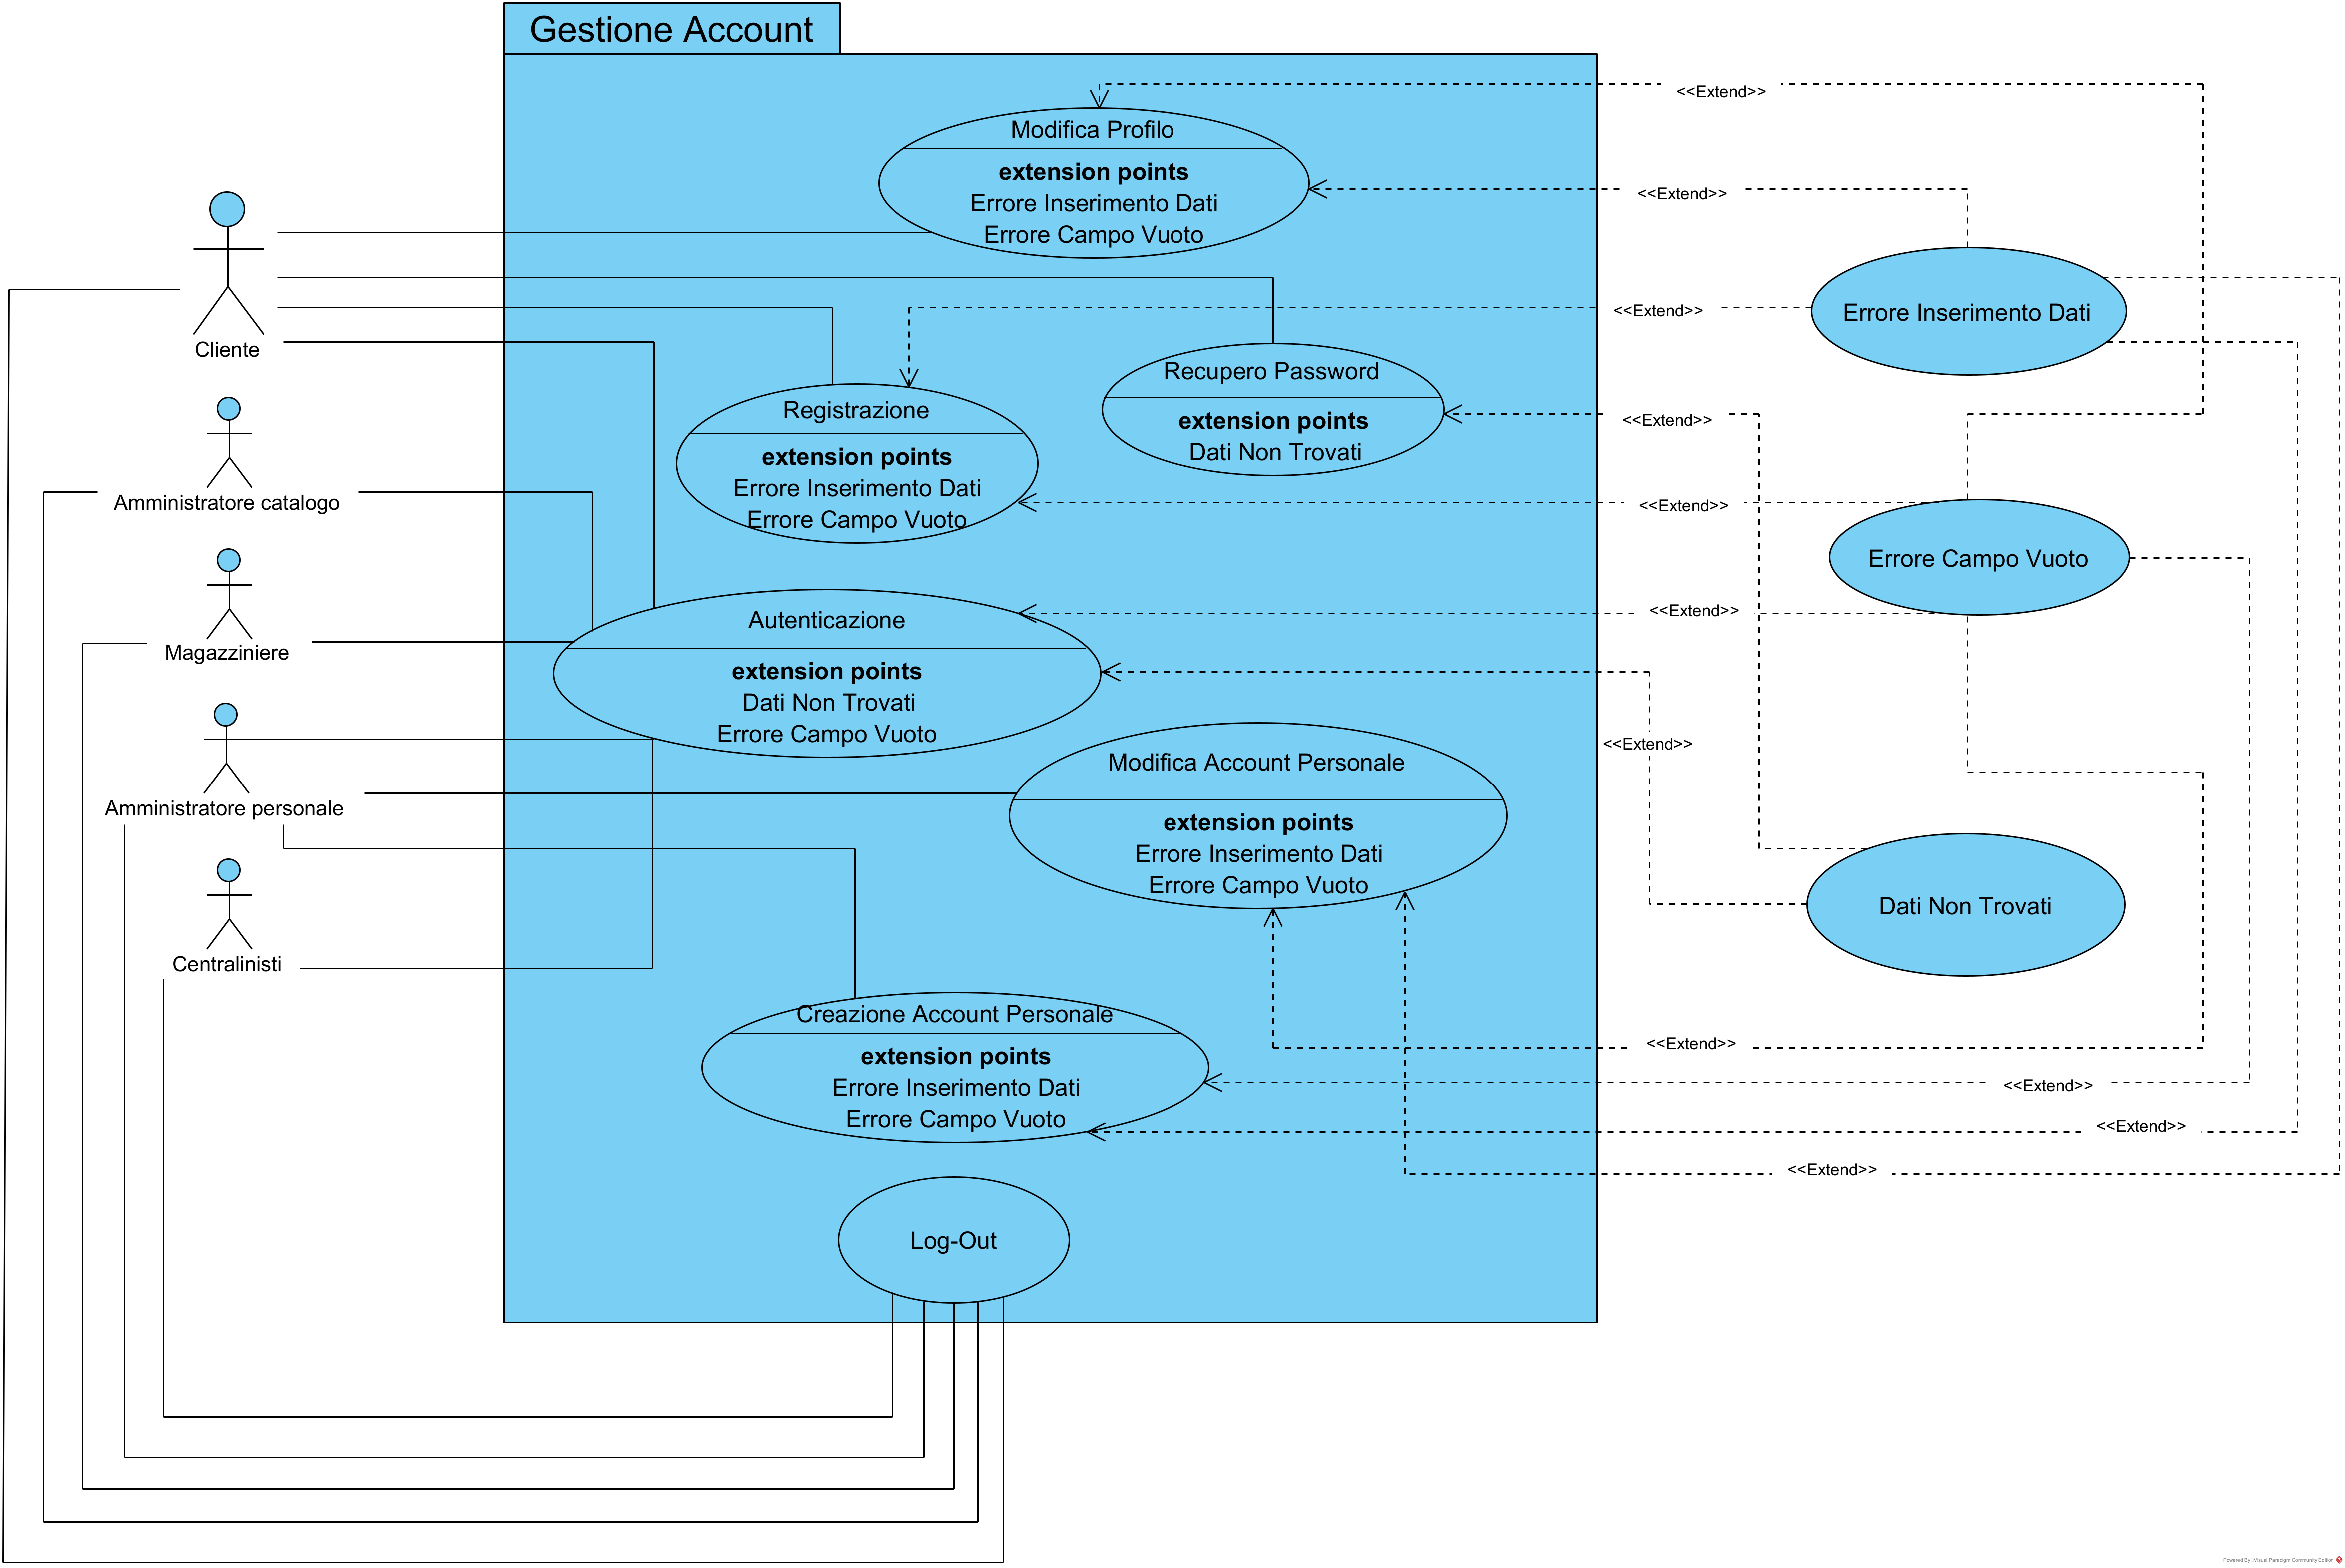
\includegraphics[width=\textwidth]{UseCase/GestioneAccount}

\subsubsection{Autenticazione di un cliente}
\label{UC:2}
\begin{tabular}{|>{\columncolor[gray]{0.8}}c|p{12cm}|}
\hline
\textbf{ID} & UC2 Autenticazione \\
\hline
\textbf{Nome} & Login di un cliente. \\
\hline
\textbf{Partecipanti} & Cliente registrato \\
\hline
\textbf{Condizione d'ingresso} & Un cliente della piattaforma visita il sito da un nuovo dispositivo. \\
\hline
\textbf{Flusso di eventi} &
\begin{minipage}{12cm}
\begin{tabular}{p{5.5cm} p{5.5cm}}
\textbf{Cliente} & \textbf{Sistema} \\
Si collega al sito, nella homepage fa click sul tasto "Login" & \\
& Mostra al cliente il form per il login, chiedendo email e password. \\
Inserisce tutti i suoi dati, fa click su "Login". & \\
& Se le credenziali sono corrette, reindirizza il cliente alla homepage. \\
\end{tabular}
\end{minipage} \\

\hline
\textbf{Condizione d'uscita} & Il cliente effettua il login. \\
\hline
\end{tabular}
\\ 

\bigskip
Fare riferimento alla tabella \ref{UC:1d}.

\subsubsection{Possibilità di aggiungere articoli al carrello}
\label{UC:3}
\begin{tabular}{|>{\columncolor[gray]{0.8}}c|p{12cm}|}
\hline
\textbf{ID} & UC3 AggiuntaCarrello \\
\hline
\textbf{Nome} & Inserimento di un articolo nel carrello. \\
\hline
\textbf{Partecipanti} & Cliente registrato \\
\hline
\textbf{Condizione d'ingresso} & Un cliente della piattaforma vuole aggiungere un articolo al carrello, intenzionato ad acquistarlo. \\
\hline
\textbf{Flusso di eventi} &
\begin{minipage}{12cm}
\begin{tabular}{p{5.5cm} p{5.5cm}}
\textbf{Cliente} & \textbf{Sistema} \\
Dopo aver effettuato il login (\ref{UC:1}), ricerca l'articolo desiderato dalla barra di ricerca. \\
& Reindirizza il cliente all'elenco degli articoli corrispondenti alla parola cercata. \\
Fa click su uno degli articoli. \\
& Reindirizza il cliente ad una pagina con i dettagli dell'articolo selezionato. \\
Fa click su ``Aggiungi al carrello". \\
& Mostra un messaggio di conferma. \\
\end{tabular}
\end{minipage} \\
\hline
\end{tabular}

\newpage

\subsubsection{Possibilità di acquisto per clienti registrati}
\label{UC:4}
\begin{tabular}{|>{\columncolor[gray]{0.8}}c|p{12cm}|}
\hline
\textbf{ID} & UC4 Acquisto \\
\hline
\textbf{Nome} & Possibilità di acquisto per utenti registrati. \\
\hline
\textbf{Partecipanti} & Cliente registrato \\
\hline
\textbf{Condizione d'ingresso} & Un cliente della piattaforma vuole acquistare un articolo già presente nel suo carrello. \\
\hline
\textbf{Flusso di eventi} &
\begin{minipage}{12cm}
\begin{tabular}{p{5.5cm} p{5.5cm}}
\textbf{Cliente} & \textbf{Sistema}\\
Fa click su ``Carrello" \\
& Reindirizza il cliente alla pagina del carrello. \\
Fa click sul tasto ``Acquista". \\
& Reindirizza il cliente alla pagina di conferma dell'ordine. \\
Fa click sul tasto ``Conferma". \\
& Invia una notifica di nuovo ordine ad un magazziniere. \\
& \begin{center} \vdots \end{center} \\
& Invia al cliente una conferma di spedizione dell'articolo. \\
\end{tabular}
\end{minipage} \\

\hline
\textbf{Condizione d'uscita} & Il cliente ha acquistato un articolo. \\

\hline
\end{tabular}


\label{UC:4d}
\bigskip
\bigskip
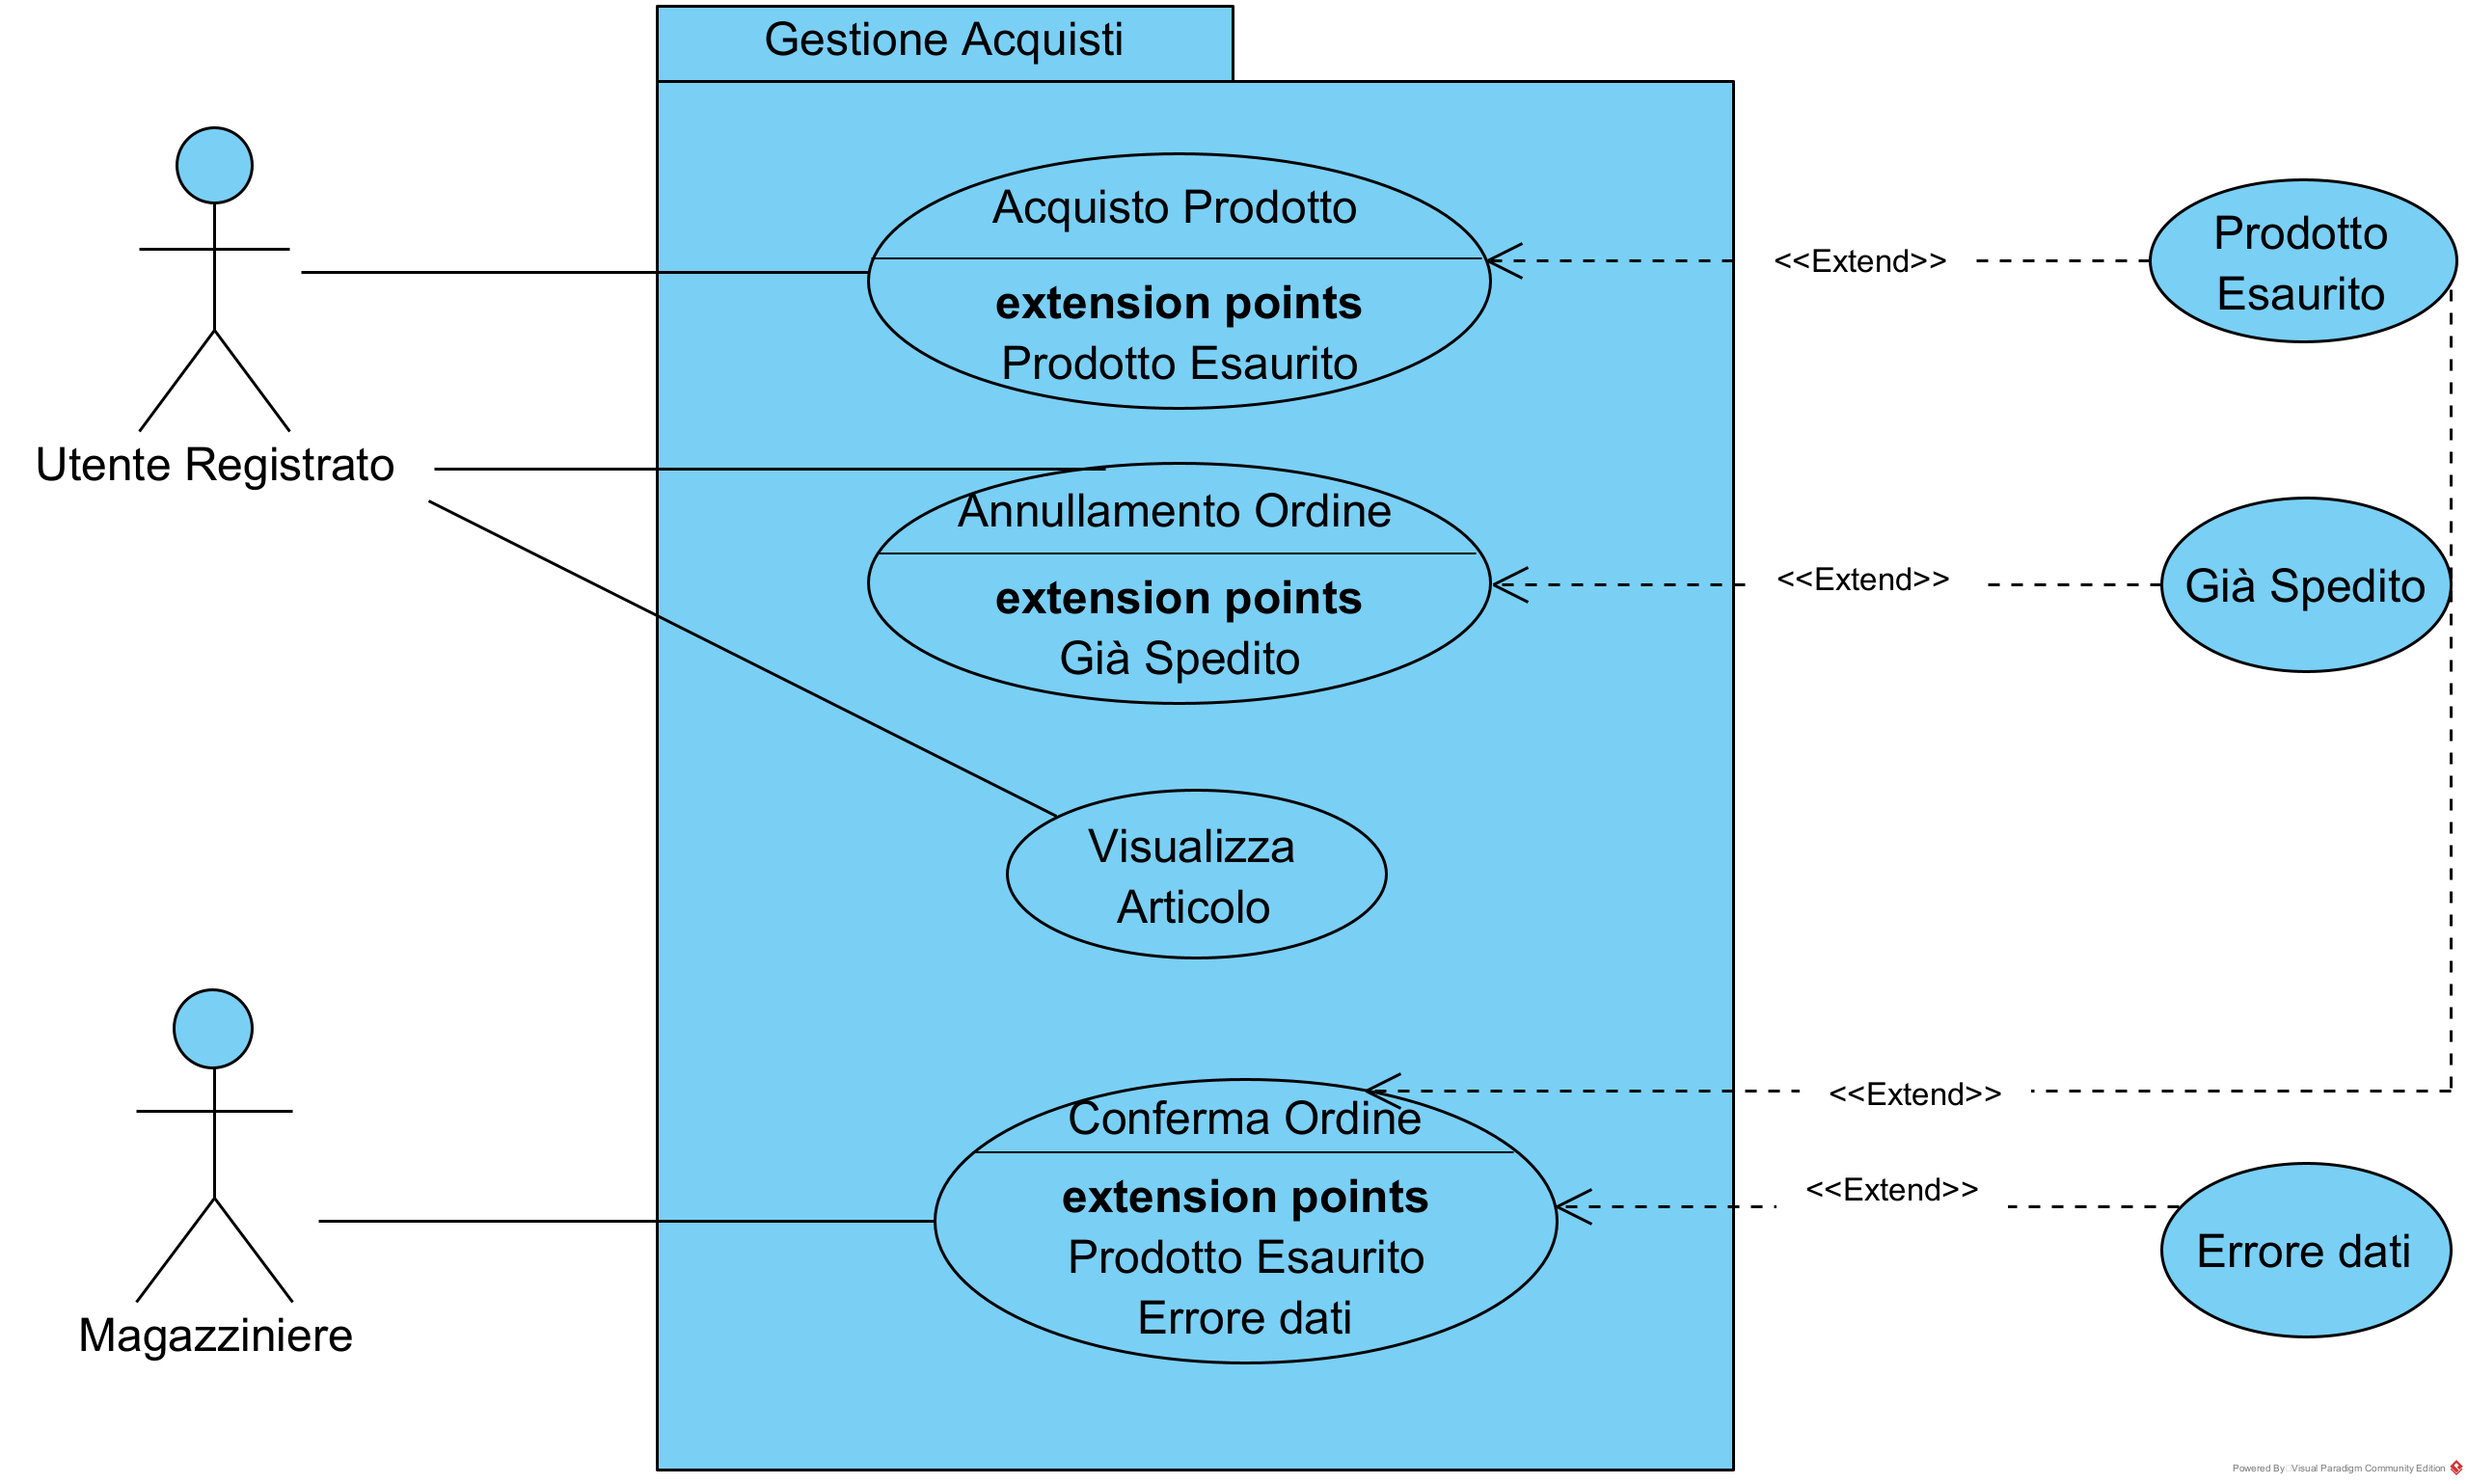
\includegraphics[height=250px]{UseCase/GestioneOrdini}

\newpage

\subsubsection{Possibilità di annullare un ordine prima che venga spedito}
\label{UC:5}
\begin{tabular}{|>{\columncolor[gray]{0.8}}c|p{12cm}|}
\hline
\textbf{ID} & UC5 Annullamento \\
\hline
\textbf{Nome} & Annullamento di un ordine. \\
\hline
\textbf{Partecipanti} & Cliente registrato \\
\hline
\textbf{Condizione d'ingresso} & Un cliente della piattaforma decide di annullare un ordine. \\
\hline
\textbf{Flusso di eventi} &
\begin{minipage}{12cm}
\begin{tabular}{p{5.5cm} p{5.5cm}}
\textbf{Cliente} & \textbf{Sistema} \\
Dopo aver effettuato un ordine (\ref{UC:4}), fa click sul tasto ``Storico ordini". \\
& Reindirizza il cliente all'elenco degli ordini effettuati. \\
Fa click su ``Annulla" in corrispondenza dell'articolo interessato. \\
& Reindirizza il cliente ad una pagina di conferma. \\
Conferma l'annullamento. \\
& Cancella l'articolo dall'elenco degli articoli da spedire. \\
& \vdots \\
& Invia un messaggio di conferma all'utente. \\
\end{tabular}
\end{minipage} \\

\hline
\textbf{Condizione d'uscita} & L'articolo non viene spedito e viene rimesso in vendita. \\
\hline
\end{tabular}

Fare riferimento al diagramma \ref{UC:4d}.

\subsubsection{Possibilità per ogni cliente di vendere articoli}
\label{UC:6}

Fare riferimento a \ref{UC:12}. \\

\begin{tabular}{|>{\columncolor[gray]{0.8}}c|p{12cm}|}
\hline
\textbf{ID} & UC6 Vendita \\
\hline
\textbf{Nome} & Un utente richiede di vendere un articolo sulla piattaforma. \\
\hline
\textbf{Partecipanti} & Cliente registrato \\
\hline
\textbf{Condizione d'ingresso} & Un cliente della piattaforma decide di vendere un articolo. \\
\hline
\textbf{Flusso di eventi} &
\begin{minipage}{12cm}
\begin{tabular}{p{5.5cm} p{5.5cm}}
\textbf{Cliente} & \textbf{Sistema} \\
Dopo aver effettuato il login (\ref{UC:1}), fa click sul tasto ``Vendi su TecStore". \\
& Reindirizza il cliente al form per l'inserimento dei dati dell'articolo da vendere. \\
Inserisce nome, prezzo, descrizione e foto dell'articolo. \\
& Reindirizza il cliente ad una pagina di conferma. \\
Conferma la vendita. \\
& Inoltra la richiesta ad un centralinista. \\
& \vdots \\
& Riceve una notifica dell'esito.
\end{tabular}
\end{minipage} \\

\hline
\textbf{Condizione d'uscita} & L'articolo viene messo in vendita sulla piattaforma. \\
\hline
\end{tabular}

\subsubsection{Possibilità di contatto del servizio clienti}
\label{UC:7}

Fare riferimento a \ref{UC:11}.\\

\begin{tabular}{|>{\columncolor[gray]{0.8}}c|p{12cm}|}
\hline
\textbf{ID} & UC7 CreazioneTicket \\
\hline
\textbf{Nome} & Contatto servizio clienti. \\
\hline
\textbf{Partecipanti} & Cliente registrato, centralinista \\
\hline
\textbf{Condizione d'ingresso} & Un cliente della piattaforma ha necessità di assistenza. \\
\hline
\textbf{Flusso di eventi} &
\begin{minipage}{12cm}
\begin{tabular}{p{5.5cm} p{5.5cm}}
\textbf{Cliente} & \textbf{Sistema}\\
Dopo aver effettuato il login (\ref{UC:1}), fa click sul tasto ``Assistenza clienti". \\
& Reindirizza il cliente al form per l'invio di un messaggio per l'assistenza clienti. \\
Scrive il messaggio.  \\
& Inoltra il messaggio ad un centralinista. \\
\vdots & \vdots \\
& Inoltra la risposta. \\
\vdots & \vdots \\
Risponde. \\
\vdots & \vdots \\
& Inoltra la risposta. \\
\vdots & \vdots \\
\vdots & \vdots \\
Chiude il ticket. \\
\end{tabular}
\end{minipage} \\

\hline
\textbf{Condizione d'uscita} & Il problema il cliente viene dichiarato risolto e il ticket viene chiuso. \\
\hline
\end{tabular}

\bigskip
\bigskip

\label{UC:7d}

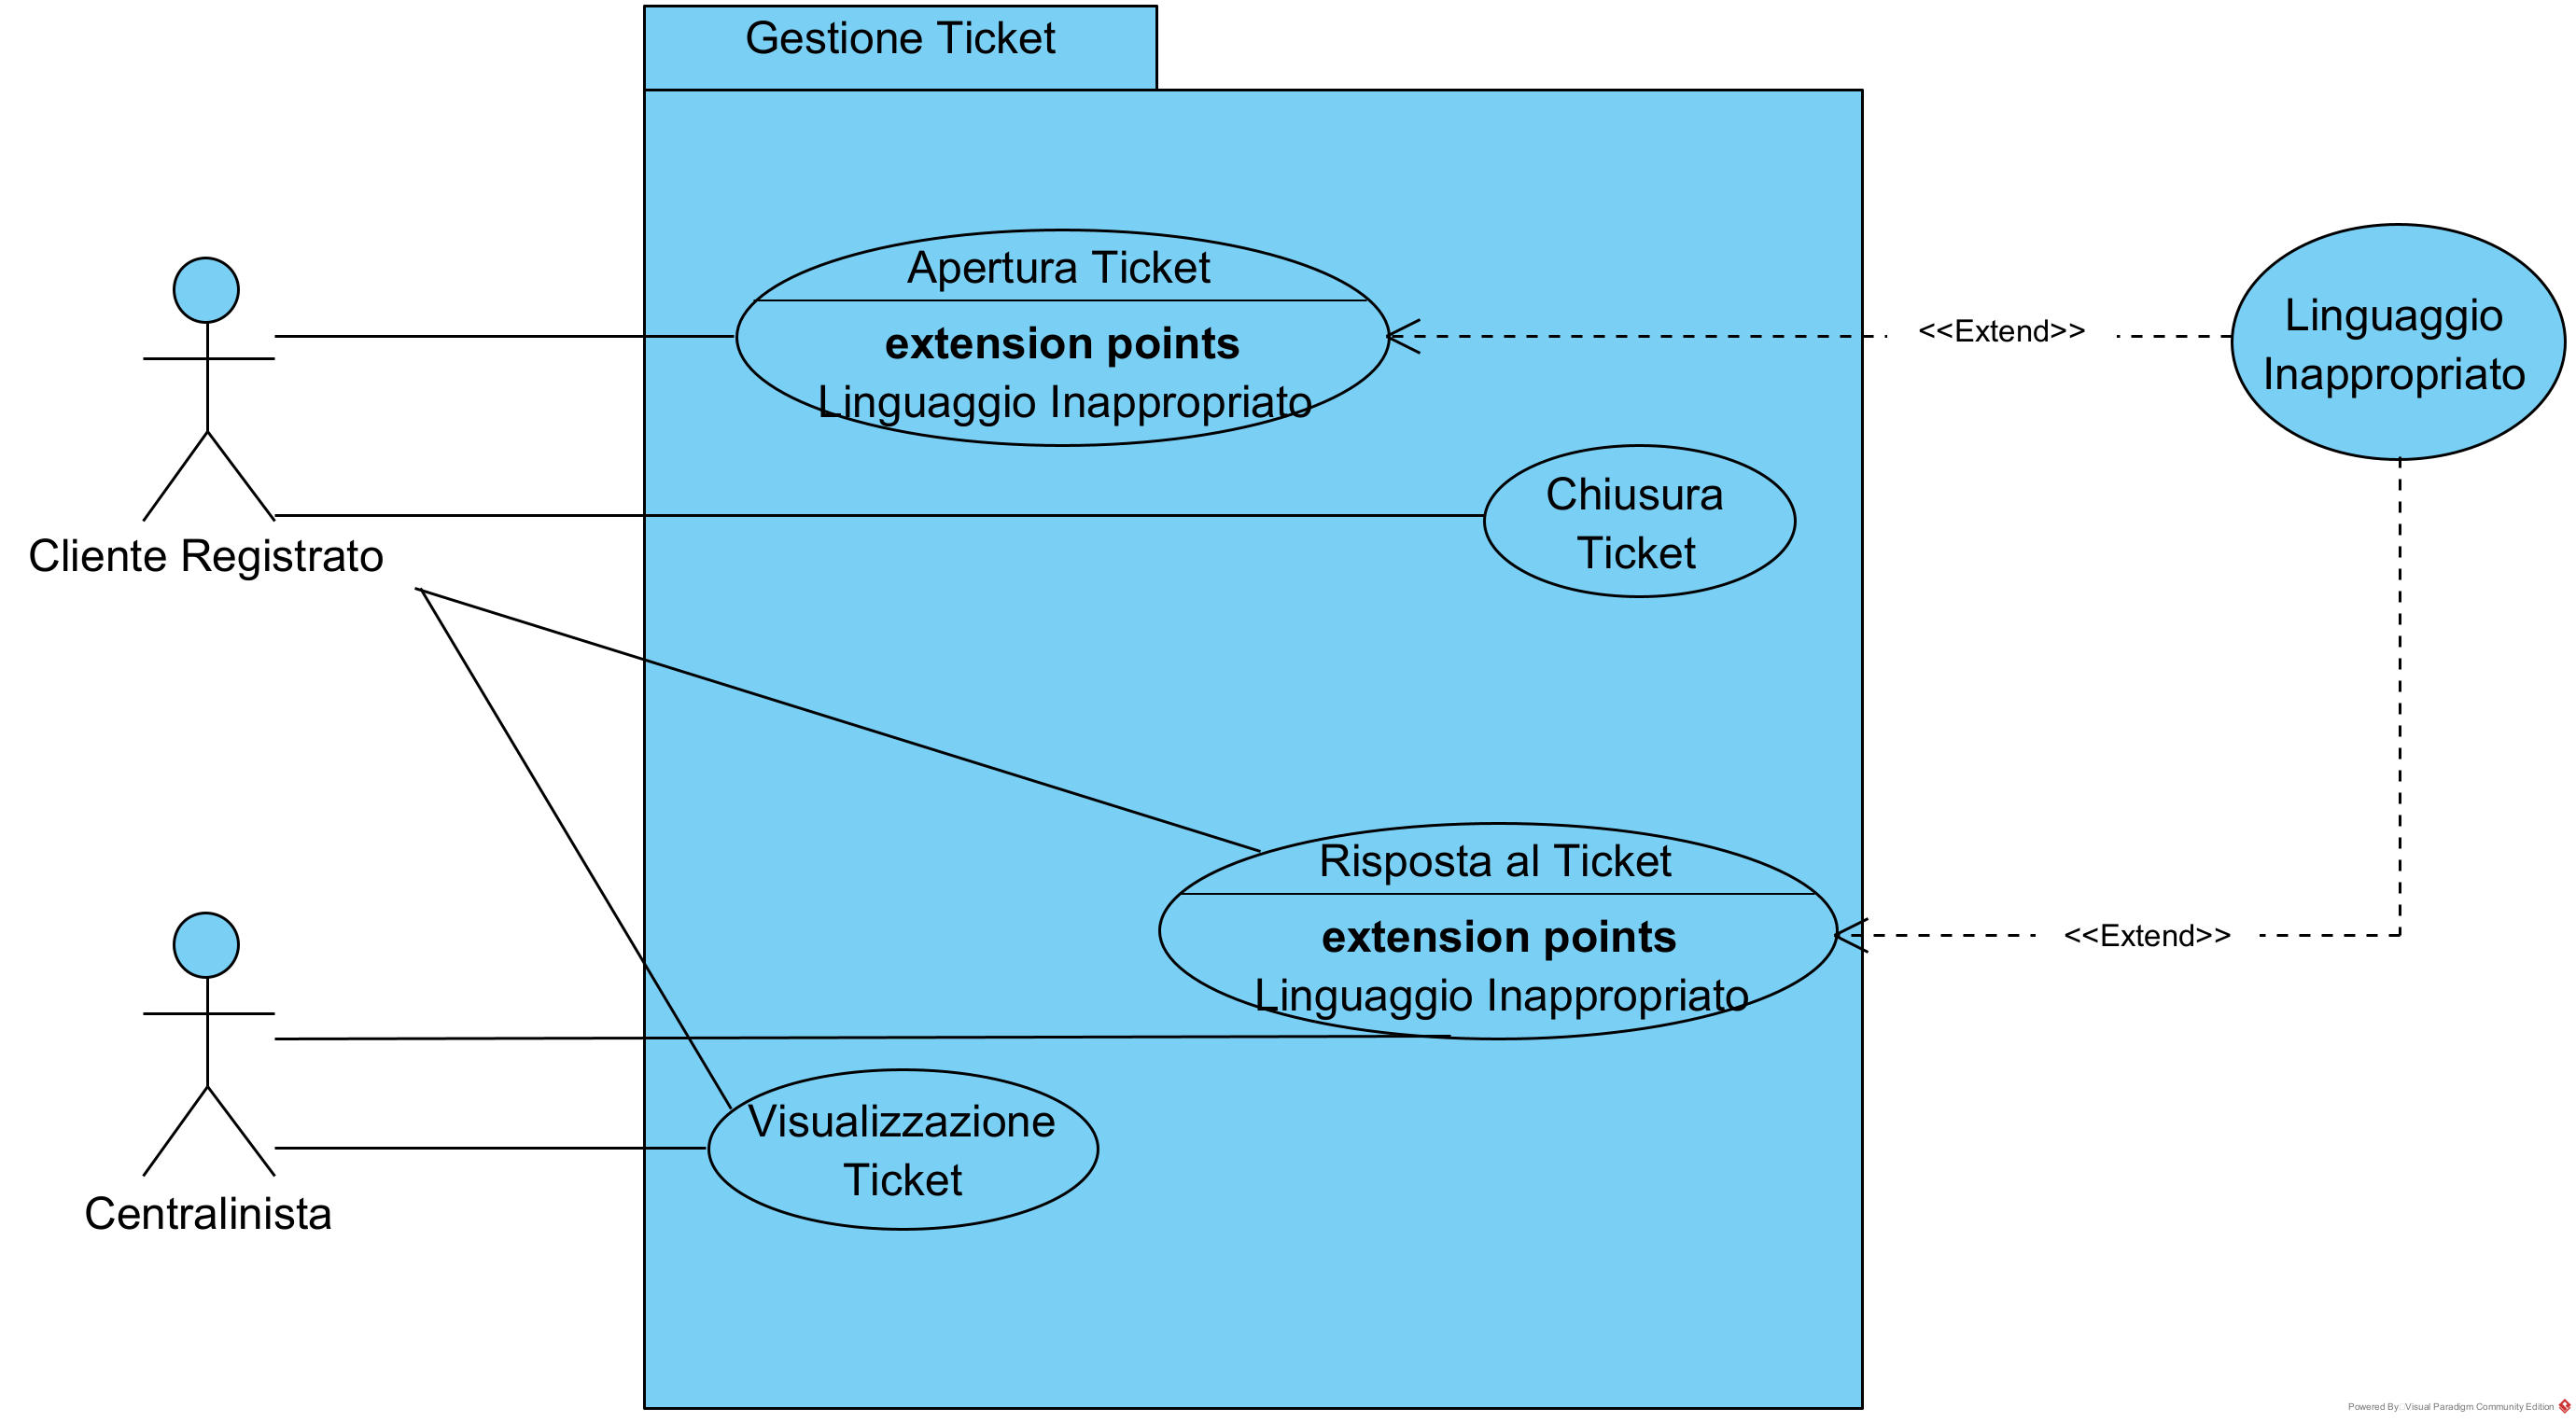
\includegraphics[height=200px]{UseCase/GestioneTicket}

\subsubsection{Modifica informazioni profilo}
\label{UC:8}
\begin{tabular}{|>{\columncolor[gray]{0.8}}c|p{12cm}|}
\hline
\textbf{ID} & UC8 ModificaProfilo \\
\hline
\textbf{Nome} & Modifica informazioni profilo. \\
\hline
\textbf{Partecipanti} & Cliente registrato \\
\hline
\textbf{Condizione d'ingresso} & Un cliente della piattaforma ha necessità di modificare le informazioni del suo profilo. \\
\hline
\textbf{Flusso di eventi} &
\begin{minipage}{12cm}
\begin{tabular}{p{5.5cm} p{5.5cm}}
\textbf{Utente} & \textbf{Sistema} \\
Dopo aver effettuato il login (\ref{UC:1}), fa click sul tasto ``Modifica profilo". \\
& Reindirizza il cliente alla contenente tutte le sue informazioni. \\
Fa click su ``Modifica".  \\
& Reindirizza il cliente ad una pagina con un form per la modifica dei dati personali. \\
Inserisce i dati modificati. \\
& Salva le modifiche. \\
\end{tabular}
\end{minipage} \\

\hline
\textbf{Condizione d'uscita} & Le vecchie informazioni vengono sovrascritte. \\
\hline
\end{tabular}

Fare riferimento alla tabella \ref{UC:1d}.

\subsubsection{Recupero password}
\label{UC:9}
\begin{tabular}{|>{\columncolor[gray]{0.8}}c|p{12cm}|}
\hline
\textbf{ID} & UC9 RecuperoPassword \\
\hline
\textbf{Nome} & Recupero password smarrita. \\
\hline
\textbf{Partecipanti} & Cliente registrato \\
\hline
\textbf{Condizione d'ingresso} & Un cliente della piattaforma ha dimenticato la sua password e vuole recuperarla. \\
\hline
\textbf{Flusso di eventi} &
\begin{minipage}{12cm}
\begin{tabular}{p{5.5cm} p{5.5cm}}
\textbf{Cliente} & \textbf{Sistema} \\
Dalla pagina del login (\ref{UC:1}), fa click su ``Password smarrita?". \\
& Reindirizza il cliente al form per l'inserimento della propria email. \\
Inserisce la propria email.  \\
& Invia un link per il recupero della password. \\
Apre la casella email e utilizza quel link. \\
&  Reindirizza il cliente ad un form per il ripristino della password. \\
Inserisce la nuova password. \\
& Reindirizza il cliente al form di login, con un messaggio che lo informa della modifica effettuata. \\
\end{tabular}
\end{minipage} \\

\hline
\textbf{Condizione d'uscita} & La password del cliente viene sovrascritta. \\
\hline
\end{tabular}

\newpage

\subsection{Gestione piattaforma}
\subsubsection{Spedizione ordini}
\label{UC:10}
Fare riferimento a \ref{UC:3} e \ref{UC:4}. \\

\begin{tabular}{|>{\columncolor[gray]{0.8}}c|p{12cm}|}
\hline
\textbf{ID} & UC10 SpedizioneOrdine \\
\hline
\textbf{Nome} & Un ordine viene spedito dal magazzino. \\
\hline
\textbf{Partecipanti} & Magazziniere \\
\hline
\textbf{Condizione d'ingresso} & Un cliente della piattaforma acquista un articolo che ora deve essere spedito. \\
\hline
\textbf{Flusso di eventi} &
\begin{minipage}{12cm}
\begin{tabular}{p{5.5cm} p{5.5cm}}
\textbf{Magazziniere} & \textbf{Sistema} \\
Dopo aver effettuato il login (\ref{UC:1}), fa click su ``Visualizza ordini" per visualizzare l'elenco degli ordini da spedire. \\
& Mostra l'elenco degli ordini. \\
Procura l'articolo dal magazzino, lo imballa, stampa la bolla di spedizione e prenota il ritiro del corriere. \\
\vdots & \vdots \\
Fa click su ``\checkmark". \\
& Reindirizza il magazziniere ad una pagina di conferma. \\
Fa click su ``Conferma". \\
& Invia una notifica al cliente. \\
\end{tabular}
\end{minipage} \\
\hline
\textbf{Condizione d'uscita} & L'articolo viene spedito. \\
\hline
\end{tabular}

\subsubsection{Gestione ticket}
\label{UC:11}
Fare riferimento a \ref{UC:7}. \\

\begin{tabular}{|>{\columncolor[gray]{0.8}}c|p{12cm}|}
\hline
\textbf{ID} & UC11 RispostaTicket \\
\hline
\textbf{Nome} & Un cliente apre un ticket. \\
\hline
\textbf{Partecipanti} & Centralinista \\
\hline
\textbf{Condizione d'ingresso} & Un cliente della piattaforma segnala un problema e un centralinista cerca di aiutarlo. \\
\hline
\textbf{Flusso di eventi} &
\begin{minipage}{12cm}
\begin{tabular}{p{5.5cm} p{5.5cm}}
\textbf{Centralinista} & \textbf{Sistema} \\
Dopo aver effettuato il login (\ref{UC:1}), fa click su ``Visualizza ticket" per visualizzare l'elenco dei ticket in attesa di risposta. \\
& Mostra l'elenco dei ticket. \\
Fa click su uno dei ticket. \\
& Mostra lo storico dei messaggi per quel ticket. \\
Scrive una risposta e preme su ``Invia". \\
& Inoltra il messaggio. \\
\vdots & \vdots \\
\end{tabular}
\end{minipage} \\
\hline
\textbf{Condizione d'uscita} & Il cliente chiude il ticket e dichiara il problema risolto. \\
\hline
\end{tabular}
\bigskip
\bigskip

Fare riferimento al diagramma \ref{UC:7d}.


\subsubsection{Controllo di ogni articolo introdotto dall'utenza}
\label{UC:12}
Fare riferimento a \ref{UC:6}. \\

\begin{tabular}{|>{\columncolor[gray]{0.8}}c|p{12cm}|}
\hline
\textbf{ID} & UC12 AutorizzazioneVendita \\
\hline
\textbf{Nome} & Un centralinista approva la vendita di un articolo. \\
\hline
\textbf{Partecipanti} & Centralinista \\
\hline
\textbf{Condizione d'ingresso} & Un cliente della piattaforma richiede di vendere una articolo. \\
\hline
\textbf{Flusso di eventi} &
\begin{minipage}{12cm}
\begin{tabular}{p{5.5cm} p{5.5cm}}
\textbf{Centralinista} & \textbf{Sistema} \\
Dopo aver effettuato il login (\ref{UC:1}), fa click su ``Visualizza vendite" per visualizzare l'elenco delle vendite in attesa di autorizzazione. \\
& Mostra l'elenco delle vendite in attesa. \\
Fa click su una delle vendite. \\
& Mostra i dettagli della vendita. \\
Fa click su \checkmark. \\
& Inoltra invia una notifica al cliente. \\
\end{tabular}
\end{minipage} \\
\hline
\textbf{Condizione d'uscita} & Il cliente chiude il ticket e dichiara il problema risolto. \\
\hline
\end{tabular}


\subsubsection{Gestione del personale da un account dedicato}
\label{UC:13}
\begin{tabular}{|>{\columncolor[gray]{0.8}}c|p{12cm}|}
\hline
\textbf{ID} & UC12 GestionePersonale \\
\hline
\textbf{Nome} & Modifica di informazioni relative al personale. \\
\hline
\textbf{Partecipanti} & Amministratore personale \\
\hline
\textbf{Condizione d'ingresso} & I dati di un dipendente devono essere modificati o deve essere aggiunto o rimosso un nuovo dipendente. \\
\hline
\textbf{Flusso di eventi} &
\begin{minipage}{12cm}
\begin{tabular}{p{5.5cm} p{5.5cm}}
\textbf{Amministratore} & \textbf{Sistema} \\
Dopo aver effettuato il login (\ref{UC:1}), fa click sul tasto opportuno per l'operazione da effettuare. \\
& Reindirizza l'amministratore alla pagina opportuna. \\
Inserisce i dati richiesti. \\
& Chiede conferma dell'operazione. \\
Conferma l'operazione. \\
\end{tabular}
\end{minipage} \\

\hline
\textbf{Condizione d'uscita} & La modifica delle informazioni del personale viene memorizzata. \\
\hline
\end{tabular}

Fare riferimento alla tabella \ref{UC:1d}.

\subsubsection{Gestione del catalogo da un account dedicato}
\label{UC:14}
\begin{tabular}{|>{\columncolor[gray]{0.8}}c|p{12cm}|}
\hline
\textbf{ID} & UC14 GestioneCatalogo \\
\hline
\textbf{Nome} & Modifica di informazioni relative al catalogo. \\
\hline
\textbf{Partecipanti} & Amministratore catalogo \\
\hline
\textbf{Condizione d'ingresso} & I dati di un dipendente devono essere modificati o deve essere aggiunto o rimosso un nuovo dipendente. \\
\hline
\textbf{Flusso di eventi} &
\begin{minipage}{12cm}
\begin{tabular}{p{5.5cm} p{5.5cm}}
\textbf{Amministratore} & \textbf{Sistema} \\
Dopo aver effettuato il login (\ref{UC:1}), fa click sul tasto opportuno per l'operazione da effettuare. \\
& Reindirizza l'amministratore alla pagina opportuna. \\
Inserisce i dati richiesti. \\
& Chiede conferma dell'operazione. \\
Conferma l'operazione. \\
\end{tabular}
\end{minipage} \\

\hline
\textbf{Condizione d'uscita} & La modifica delle informazioni del catalogo viene memorizzata. \\
\hline
\end{tabular}

\section{Class Diagram}
e\includegraphics[width=\textwidth]{diagrammadiclasse}

\newpage
\section{Sequence Diagram}
\subsection{Registrazione di un cliente}

Fare riferimento a \ref{UC:1}.

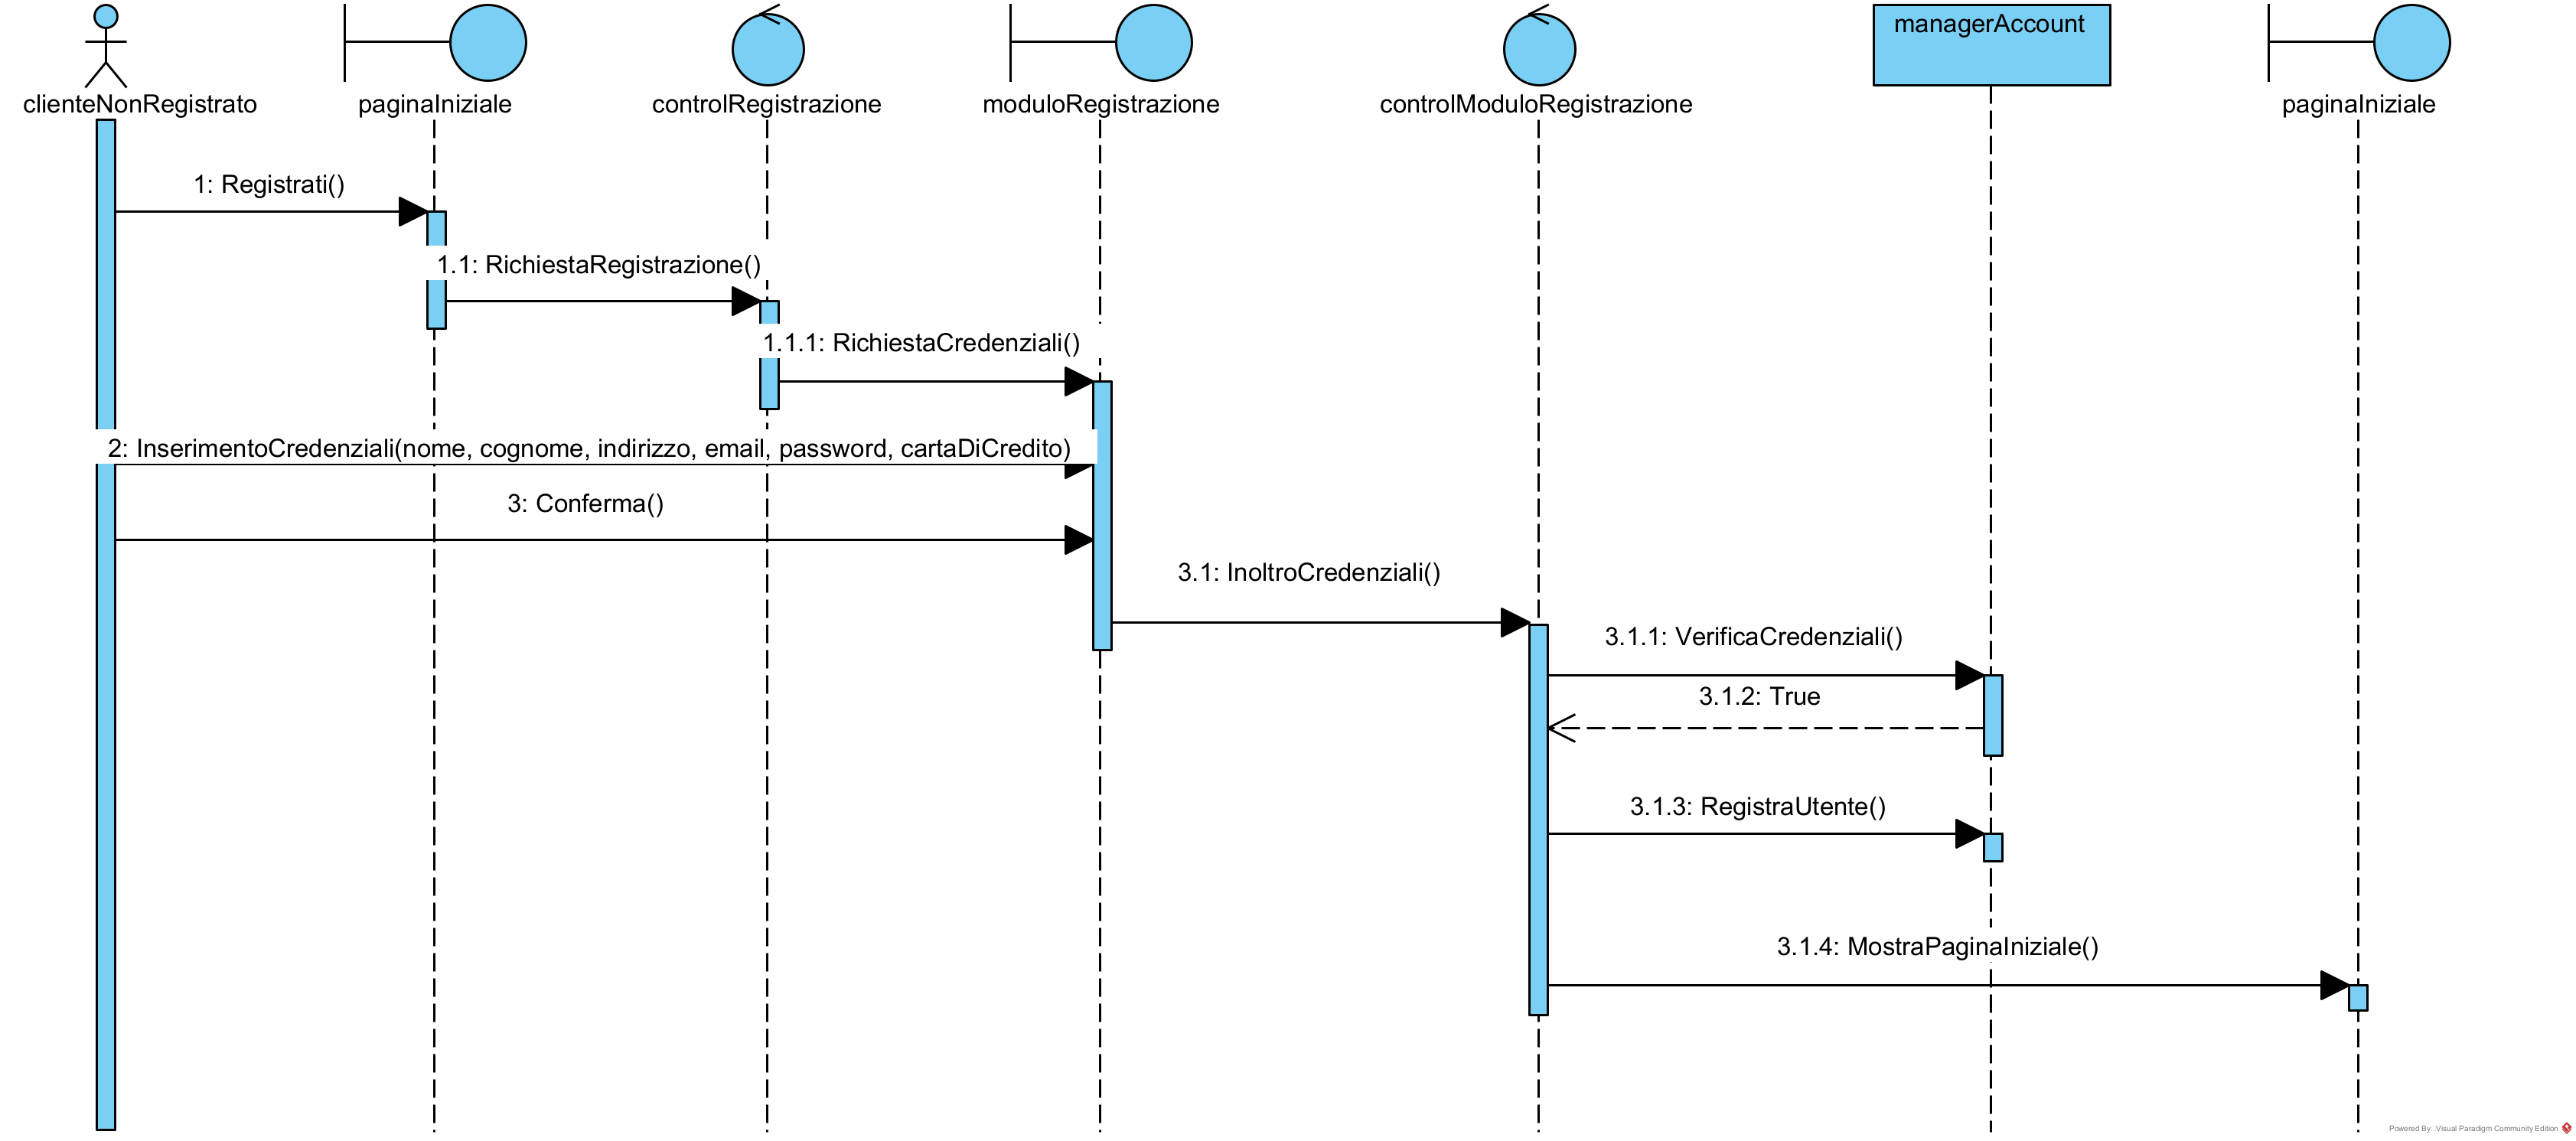
\includegraphics[height=200px]{SequenceDiagram/Registrazione}

\begin{enumerate}
\item Un nuovo cliente della piattaforma desidera registrarsi al sito e fa click sul tasto ``Registrati".
\item Il boundary ``Pagina Iniziale" inoltra la richiesta al control Registrazione, che reindirizza l'utente al boundary con il modulo per la registrazione.
\item L'utente inserisce i dati richiesti e conferma la registrazione.
\item Il ``controlModuloRegistrazione" inoltra i dati al ``managerAccount" per verificare che i dati siano corretti e non duplicati.
\item Se i dati sono corretti, chiede al manager di registrare l'utente.
\item Il control effettua il login per l'utente e lo reindirizza alla pagina iniziale.
\end{enumerate}

\newpage

\subsection{Acquisto}

Fare riferimento a \ref{UC:4}.

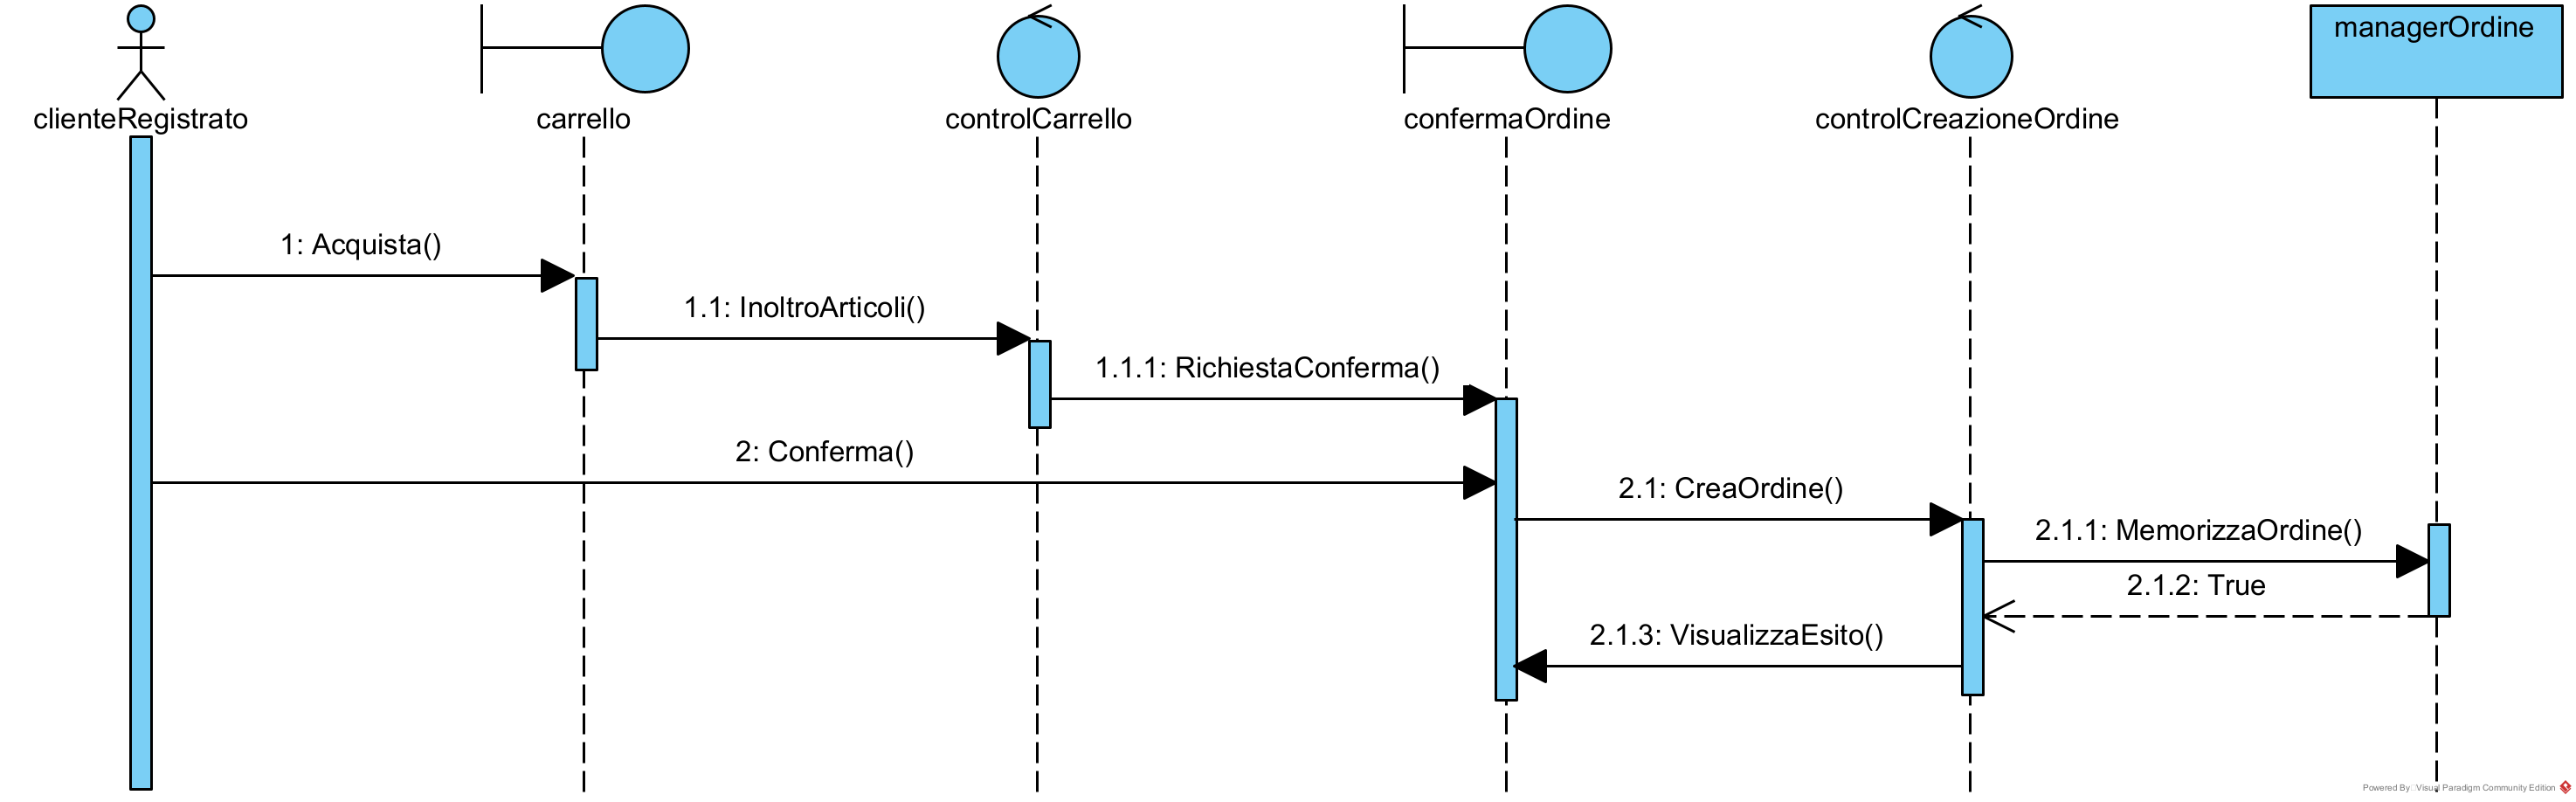
\includegraphics[width=\textwidth]{SequenceDiagram/Acquisto}

\begin{enumerate}
\item Un utente ha precedentemente aggiunto un articolo al carrello ed ha deciso di effettuare l'ordine. Dal boundary ``Carrello" fa click su ``Acquista".
\item Il contenuto del carrello viene inoltrato al controlCarrello, che reindirizza l'utente ad un boundary in cui viene chiesto all'utente di confermare i dati dell'acquisto.
\item Se l'utente conferma, l'elenco viene inoltrato al controlCreazioneOrdine che comunica al managerOrdine di memorizzare gli articoli richiesti.
\item All'utente viene mostrato l'esito della creazione dell'ordine.
\end{enumerate}

\newpage

\subsection{Annullamento}

Fare riferimento a \ref{UC:5}.

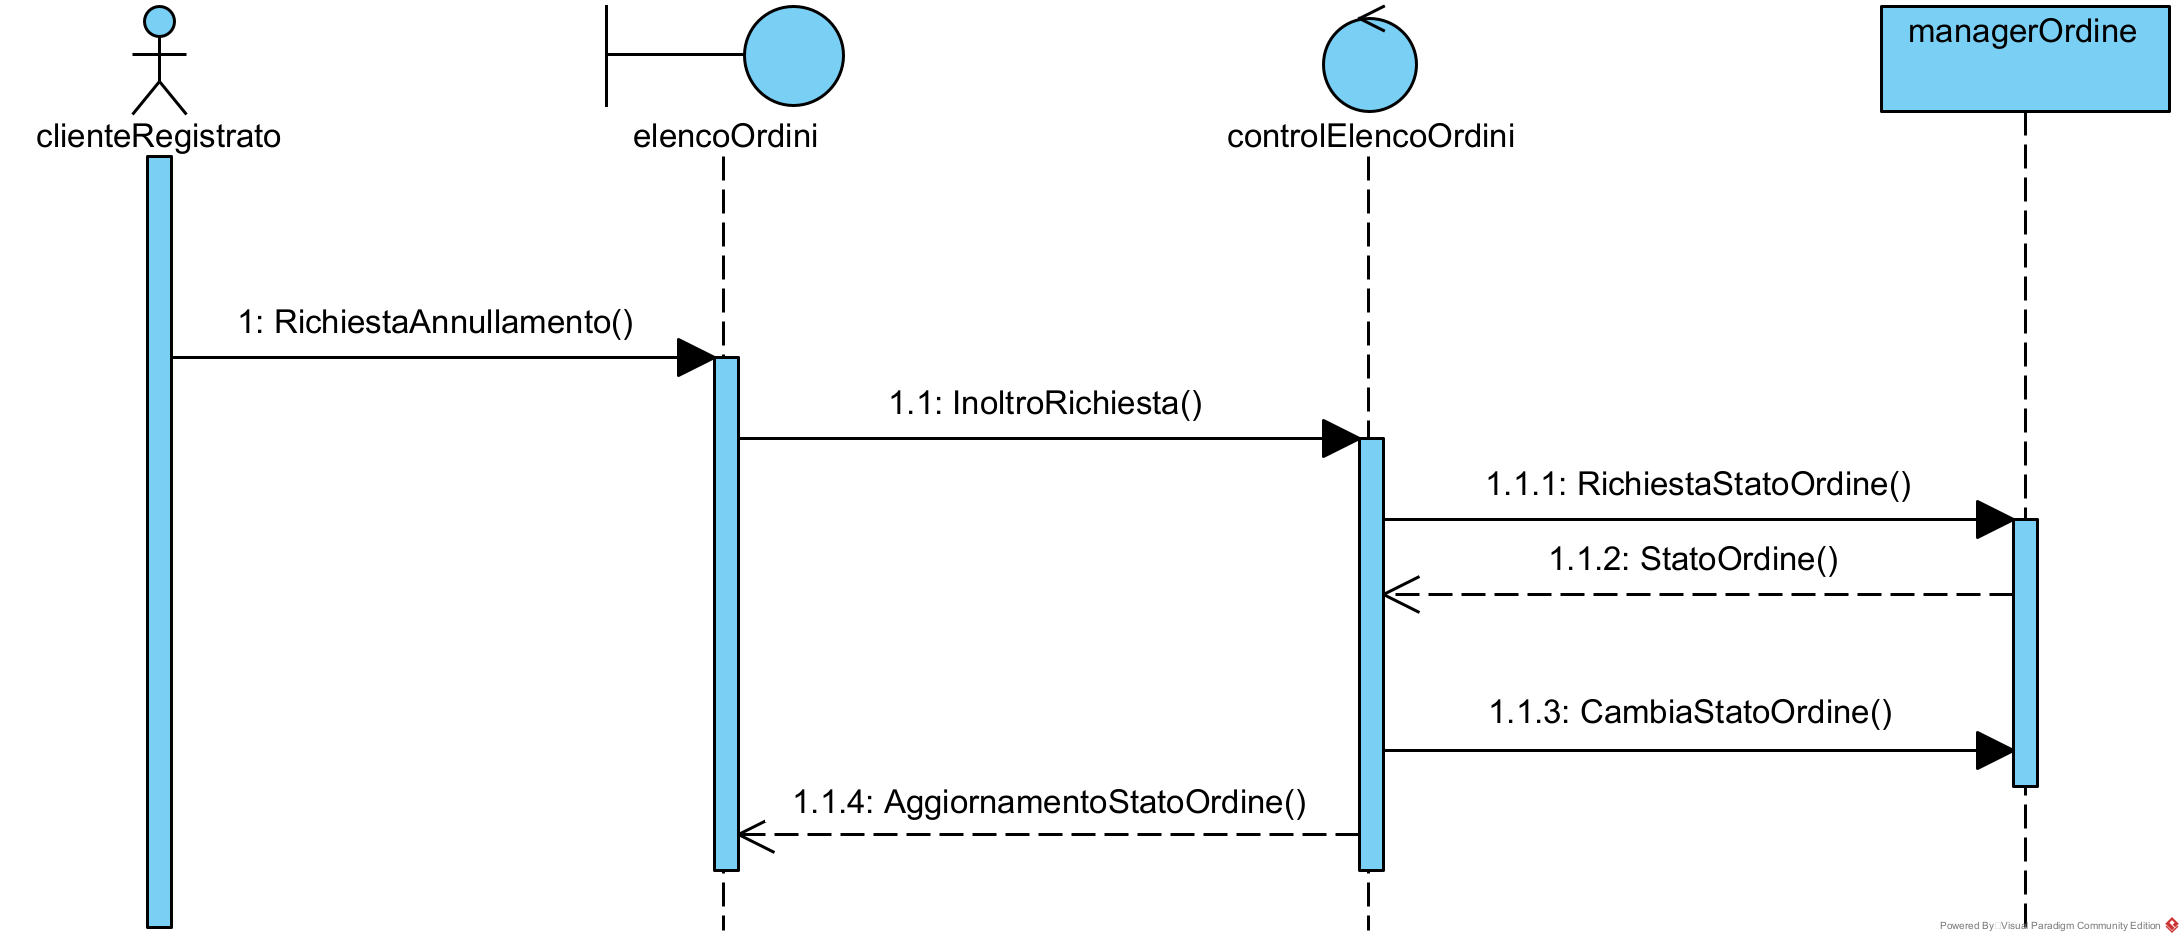
\includegraphics[height=200px]{SequenceDiagram/Annullamento}

\begin{enumerate}
\item Dalla pagina dello storico degli ordini, il cliente fa click sul tasto ``Annulla" per l'ordine interessato.
\item La richiesta viene inoltrata al controlElencoOrdini che verifica che l'ordine non sia stato già spedito. Se non lo è, cambia lo stato dell'ordine.
\item Il controlElencoOrdini visualizza una conferma all'utente.
\end{enumerate}

\subsection{Vendita}

Fare riferimento a \ref{UC:6}.

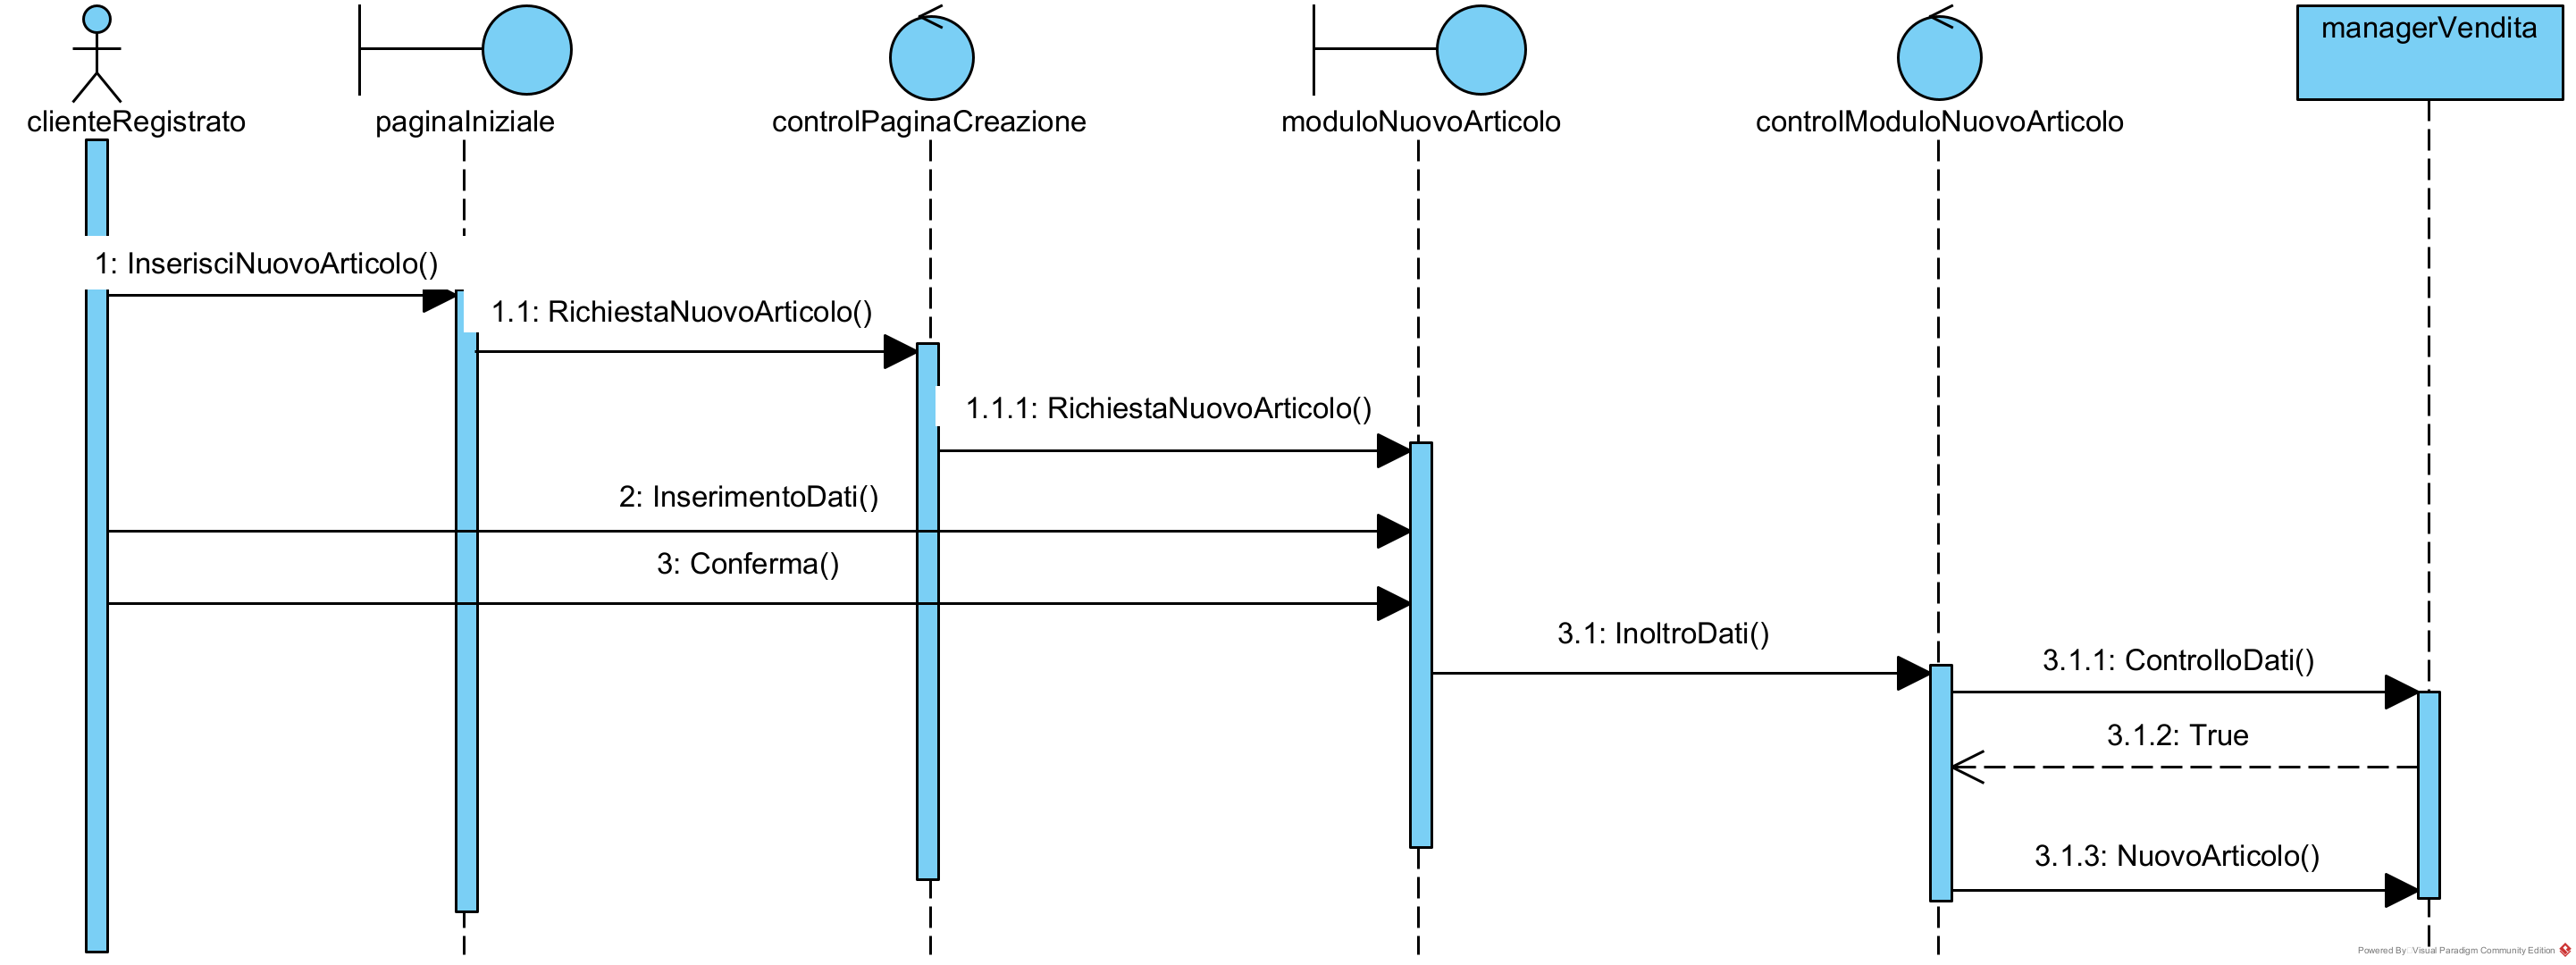
\includegraphics[height=180px]{SequenceDiagram/Vendita}

\begin{enumerate}
\item Un utente vuole vendere un articolo. Dalla pagina iniziale fa click sul tasto per creare una nuova vendita.
\item Il controlPaginaCreazione reindirizza l'utente al modulo per l'inserimento dei dati necessari.
\item L'utente inserisce i dati e conferma.
\item I dati vengono inoltrato al controlModuloNuovoArticolo che, dopo aver verificato che non ci siano problemi coi dati, chiede al manager di memorizzare il nuovo ordine.
\item L'ordine rimarrà nello stato "In attesa" finché un centralinista non effettua un'ulteriore verifica manuale.
\end{enumerate}

\subsection{Creazione ticket}

Fare riferimento a \ref{UC:7}.

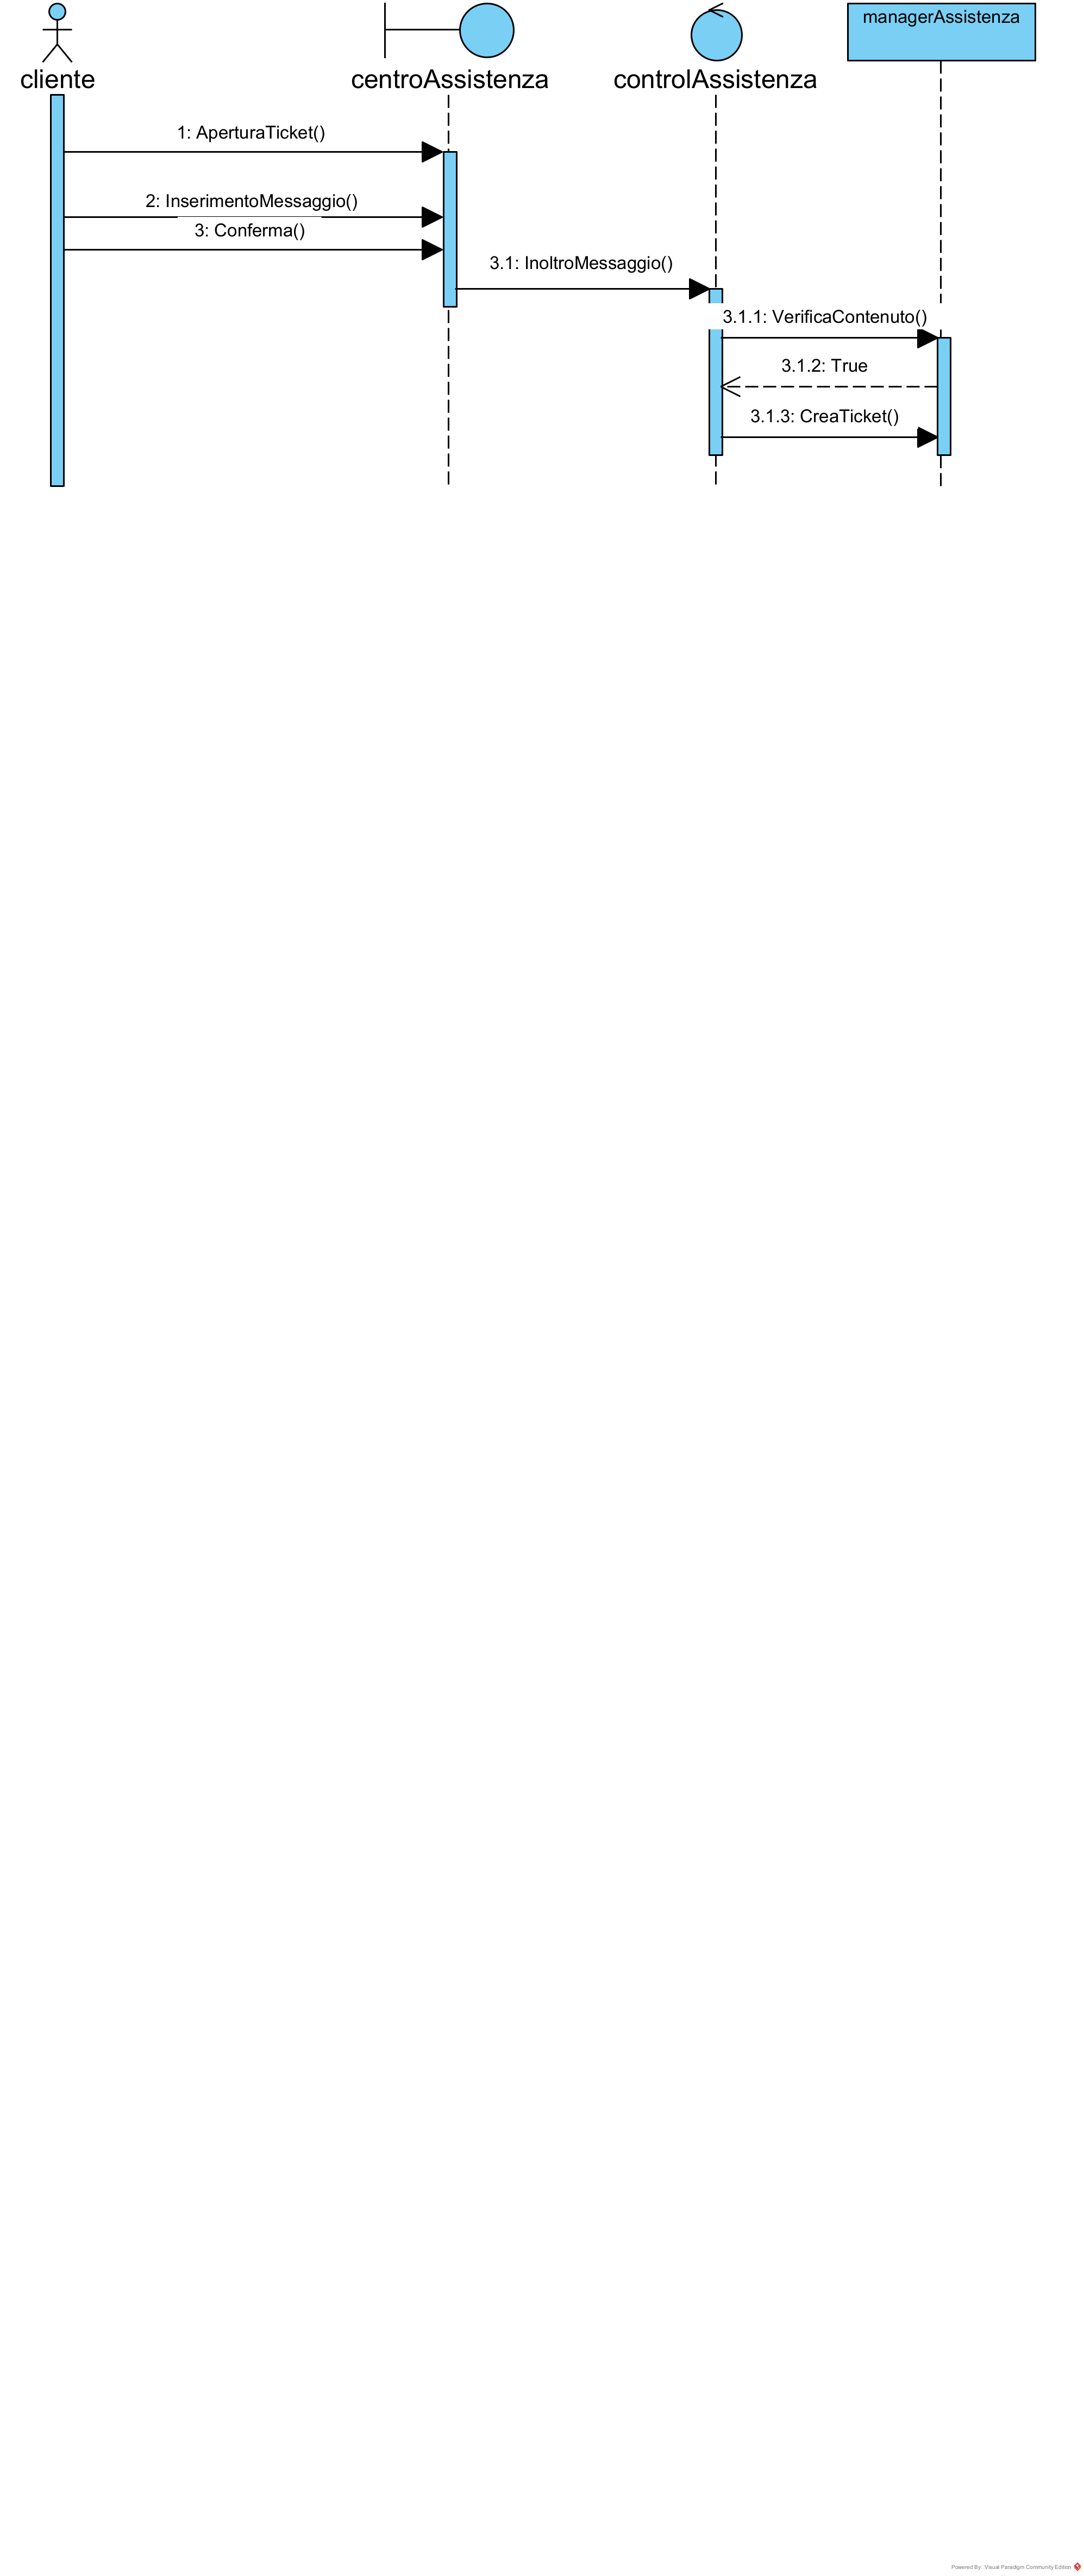
\includegraphics[height=200px]{SequenceDiagram/CreazioneTicket}

\begin{enumerate}
\item Un cliente che ha necessità di comunicare con il centro assistenza visita la pagina dedicata e fa click su ``Nuovo ticket".
\item Scrive il messaggio e fa click su ``Conferma".
\item Il messaggio viene inoltrato attraverso il controlAssistenza al managerAssistenza che verifica che il contenuto del messaggio non sia volgare o offensivo.
\item Se non lo è, memorizza il nuovo messaggio nel database.
\end{enumerate}

\subsection{Spedizione ordine}

Fare riferimento a \ref{UC:10}.

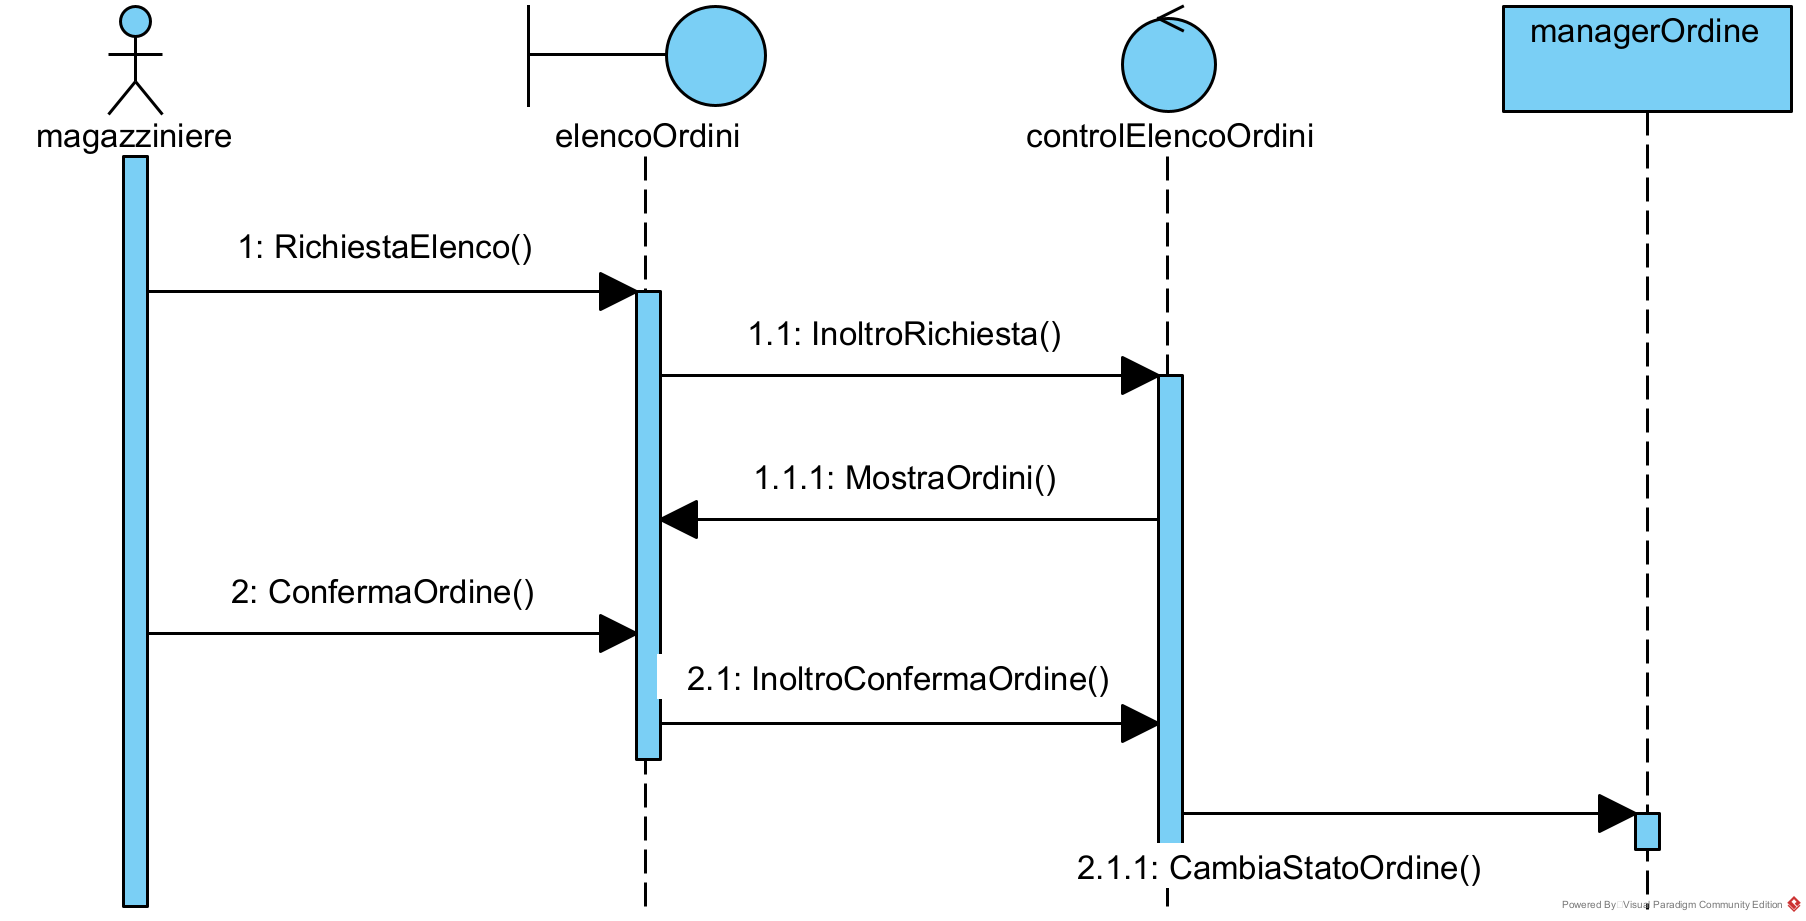
\includegraphics[height=200px]{SequenceDiagram/SpedizioneOrdine}

\begin{enumerate}
\item Dall'elenco degli ordini, il magazziniere vede un nuovo ordine da spedire.
\item Dopo aver effettuato le dovute procedure, come imballaggio, prenotazione corriere, stampa dell'etichetta, conferma la spedizione.
\item Il controlElencoOrdini inoltra il cambio di stato al managerOrdine.
\end{enumerate}

\subsection{Autorizzazione vendita}

Fare riferimento a \ref{UC:12}.

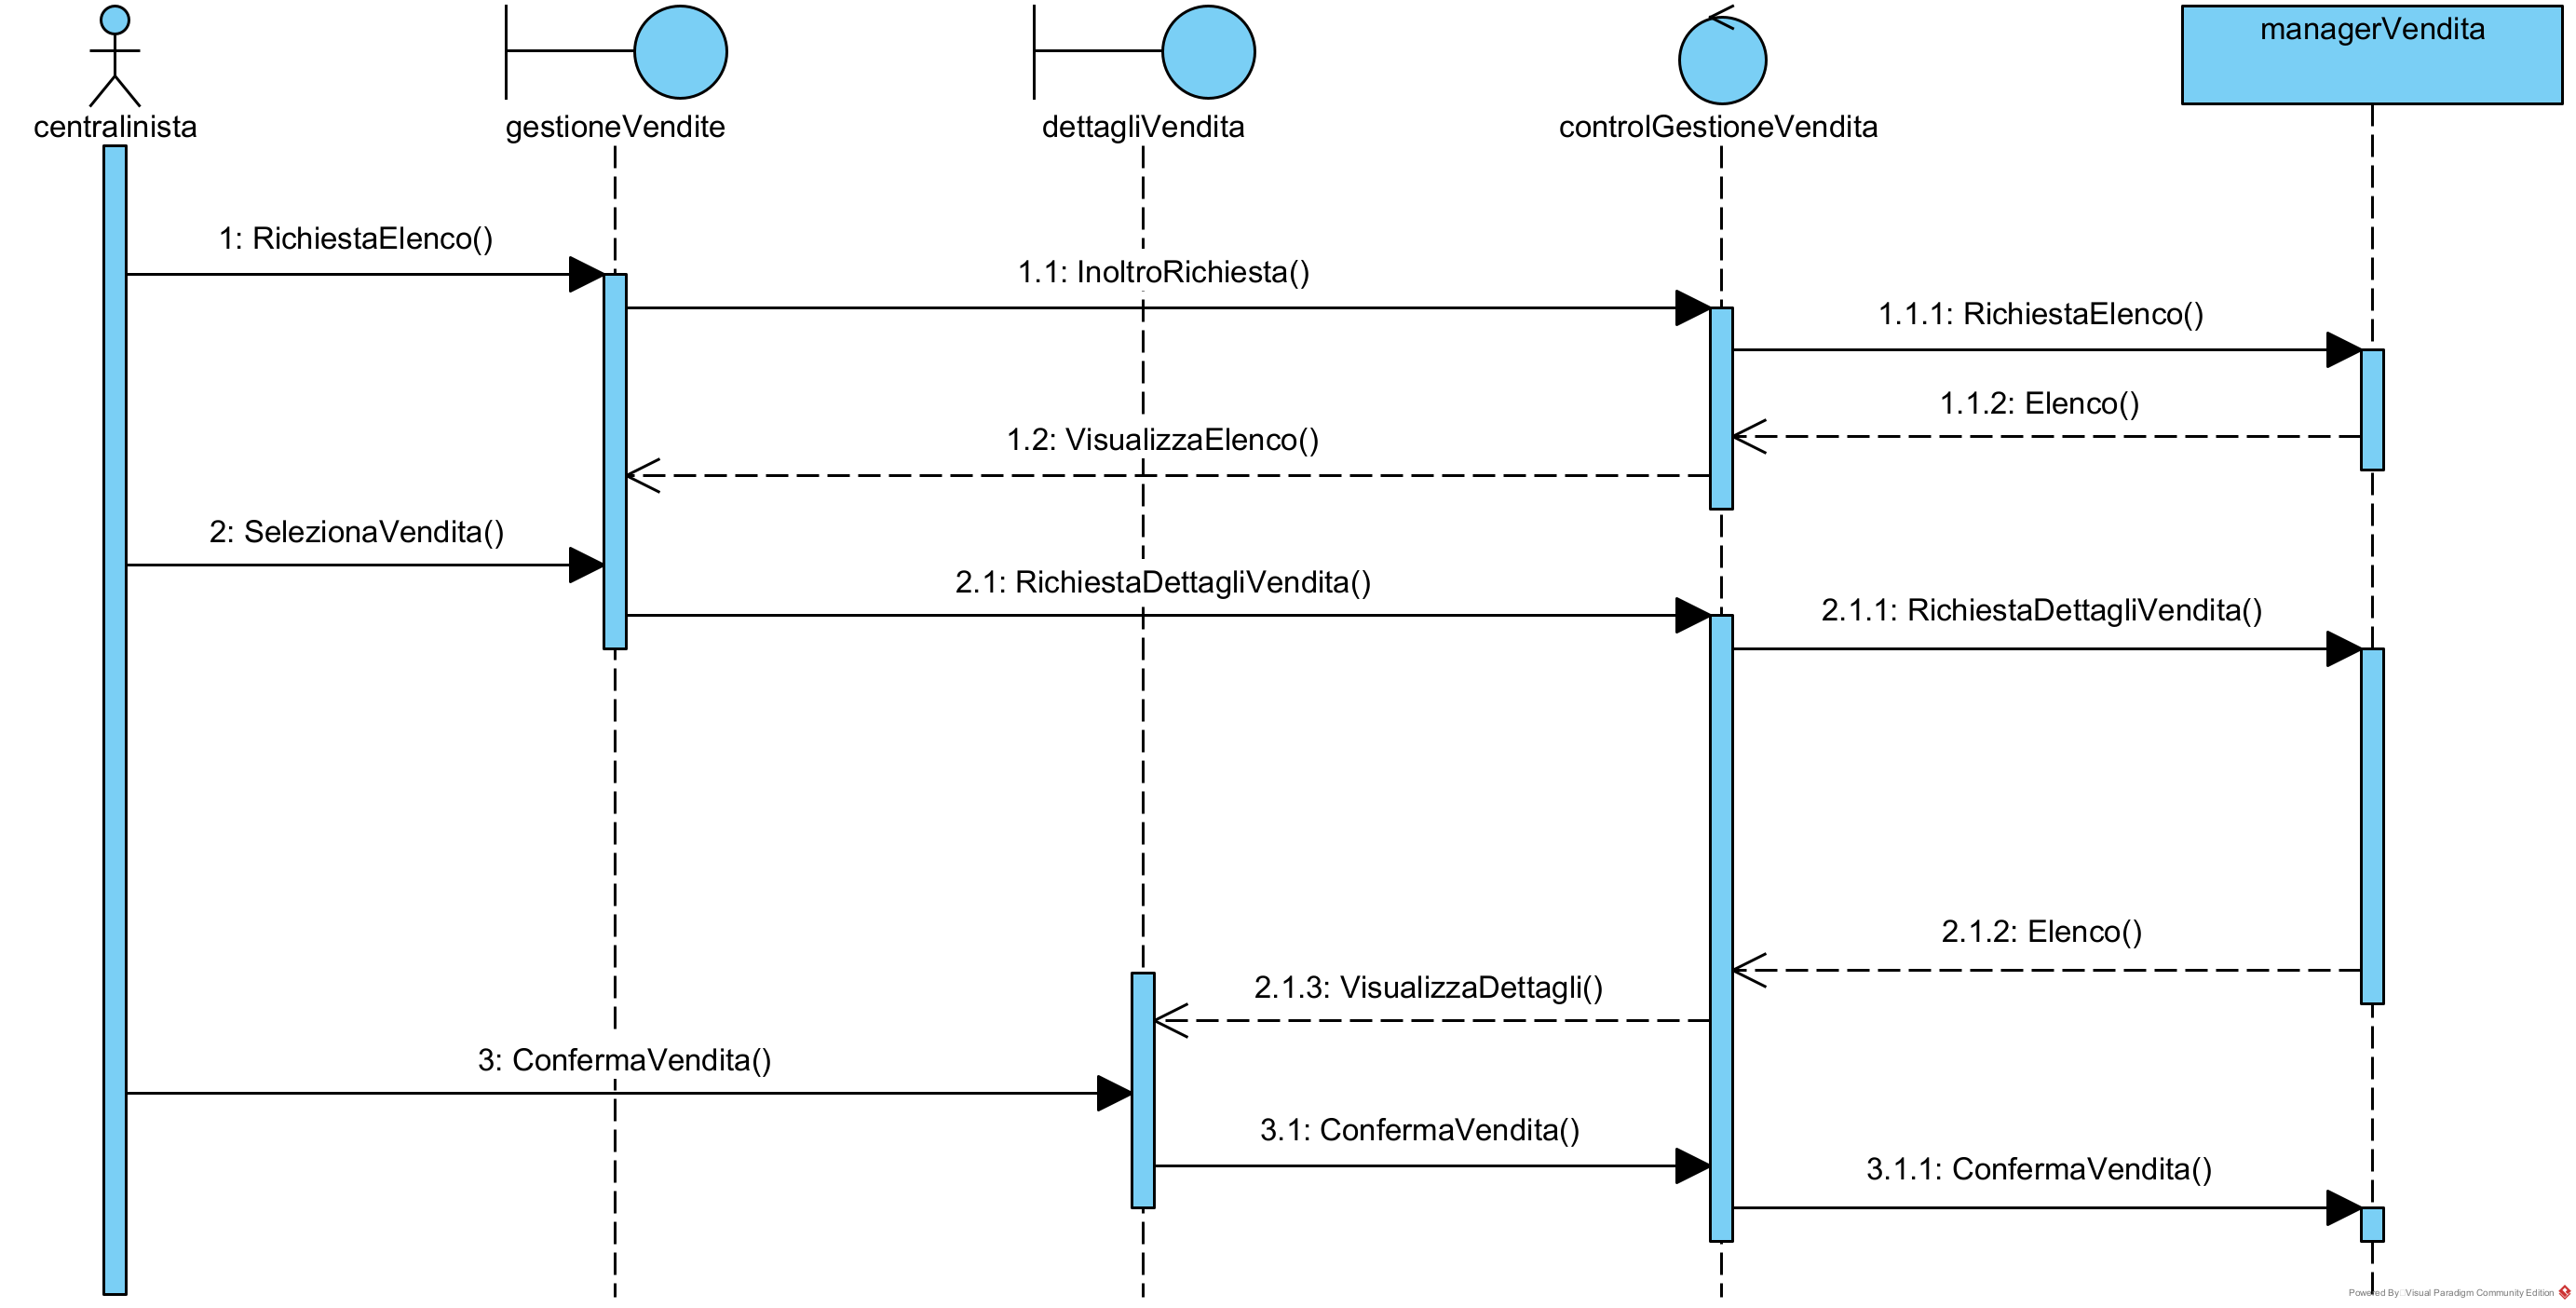
\includegraphics[height=250px]{SequenceDiagram/AutorizzazioneVendita}

\begin{enumerate}
\item Dall'elenco degli articoli in attesa di conferma, un centralinista sceglie uno degli articoli.
\item Il centralinista viene reindirizzato ad una pagina con i dettagli della vendita.
\item Se tutto risulta in regola, il centralinista conferma la vendita e il controlGestioneVendita inoltra la richiesta al managerVendita.
\end{enumerate}

\newpage

\subsection{Gestione del personale}

Fare riferimento a \ref{UC:13}.

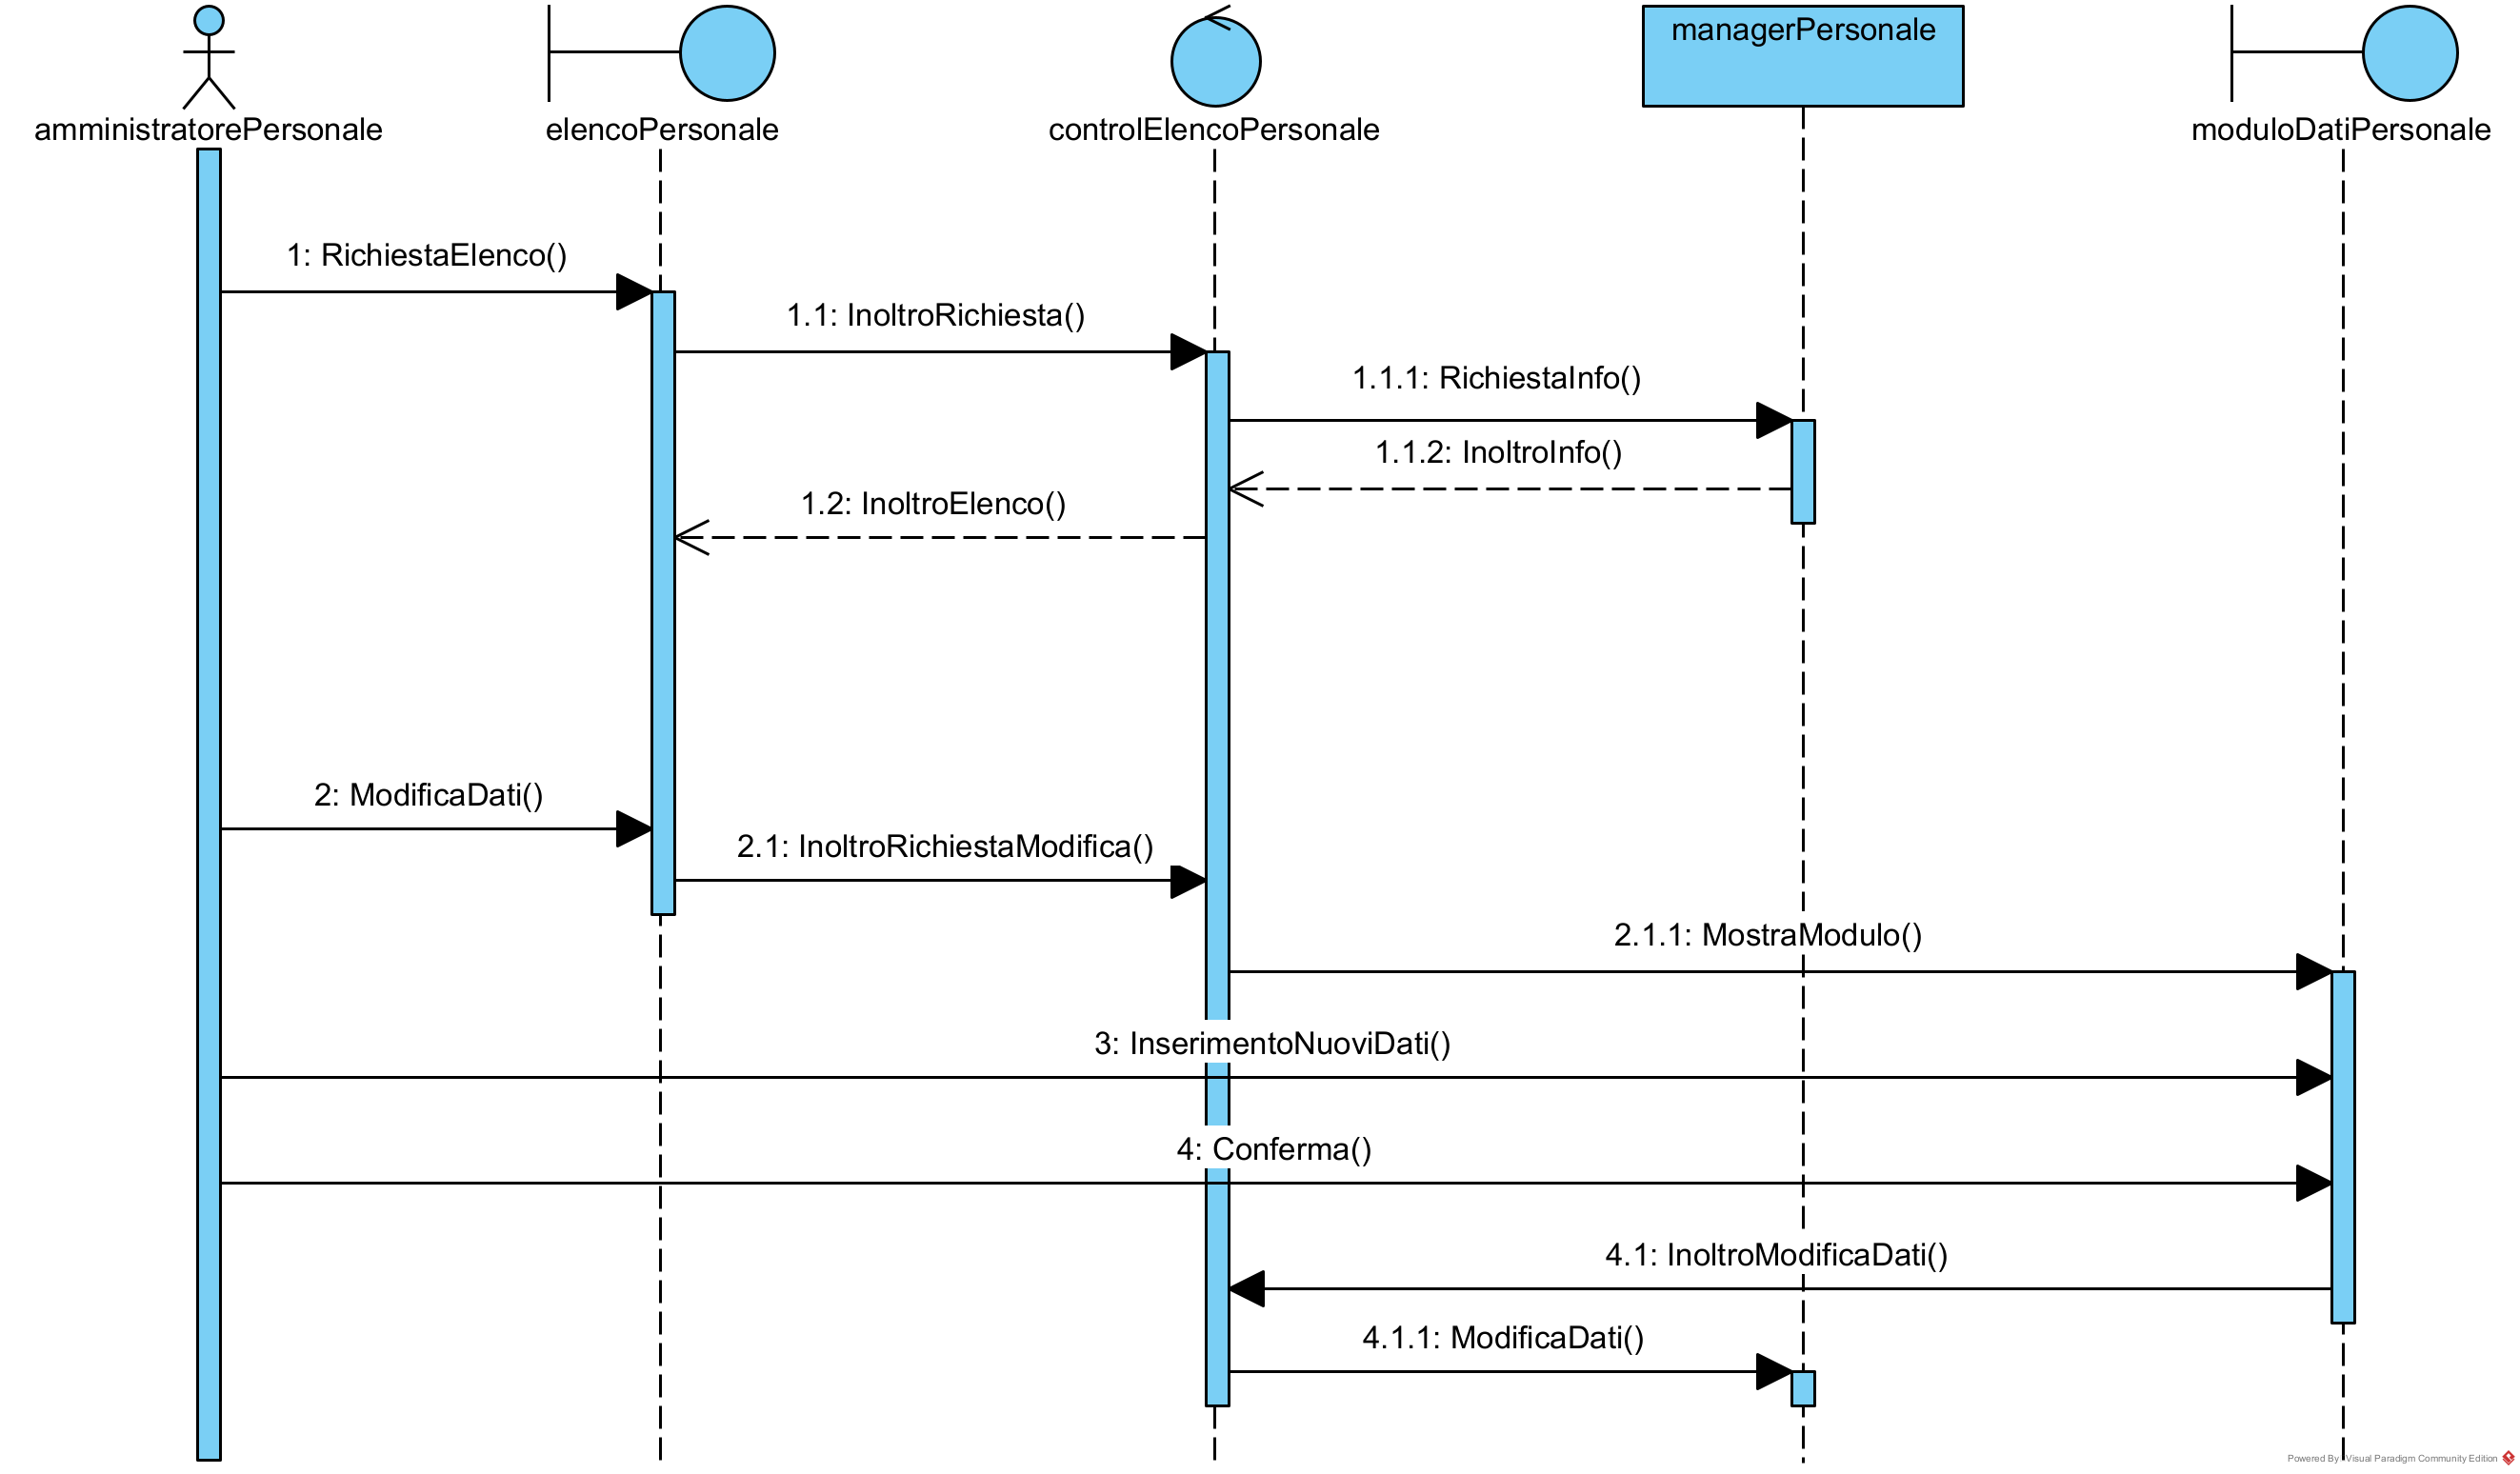
\includegraphics[height=250px]{SequenceDiagram/GestionePersonale}

\begin{enumerate}
\item Dall'elenco dei dipendenti, un amministratore fa click sul dipendente di cui vuole modificare i dati.
\item Attraverso il controlElencoPersonale, l'amministratore viene reindirizzato ad un modulo in cui modificare i dati.
\item Una volta confermati i dati, il controlElencoPersonale inoltra la richiesta di modifica al managerPersonale, che salva le nuove informazioni nel database.
\end{enumerate}

\newpage

\subsection{Gestione del catalogo}

Fare riferimento a \ref{UC:14}.

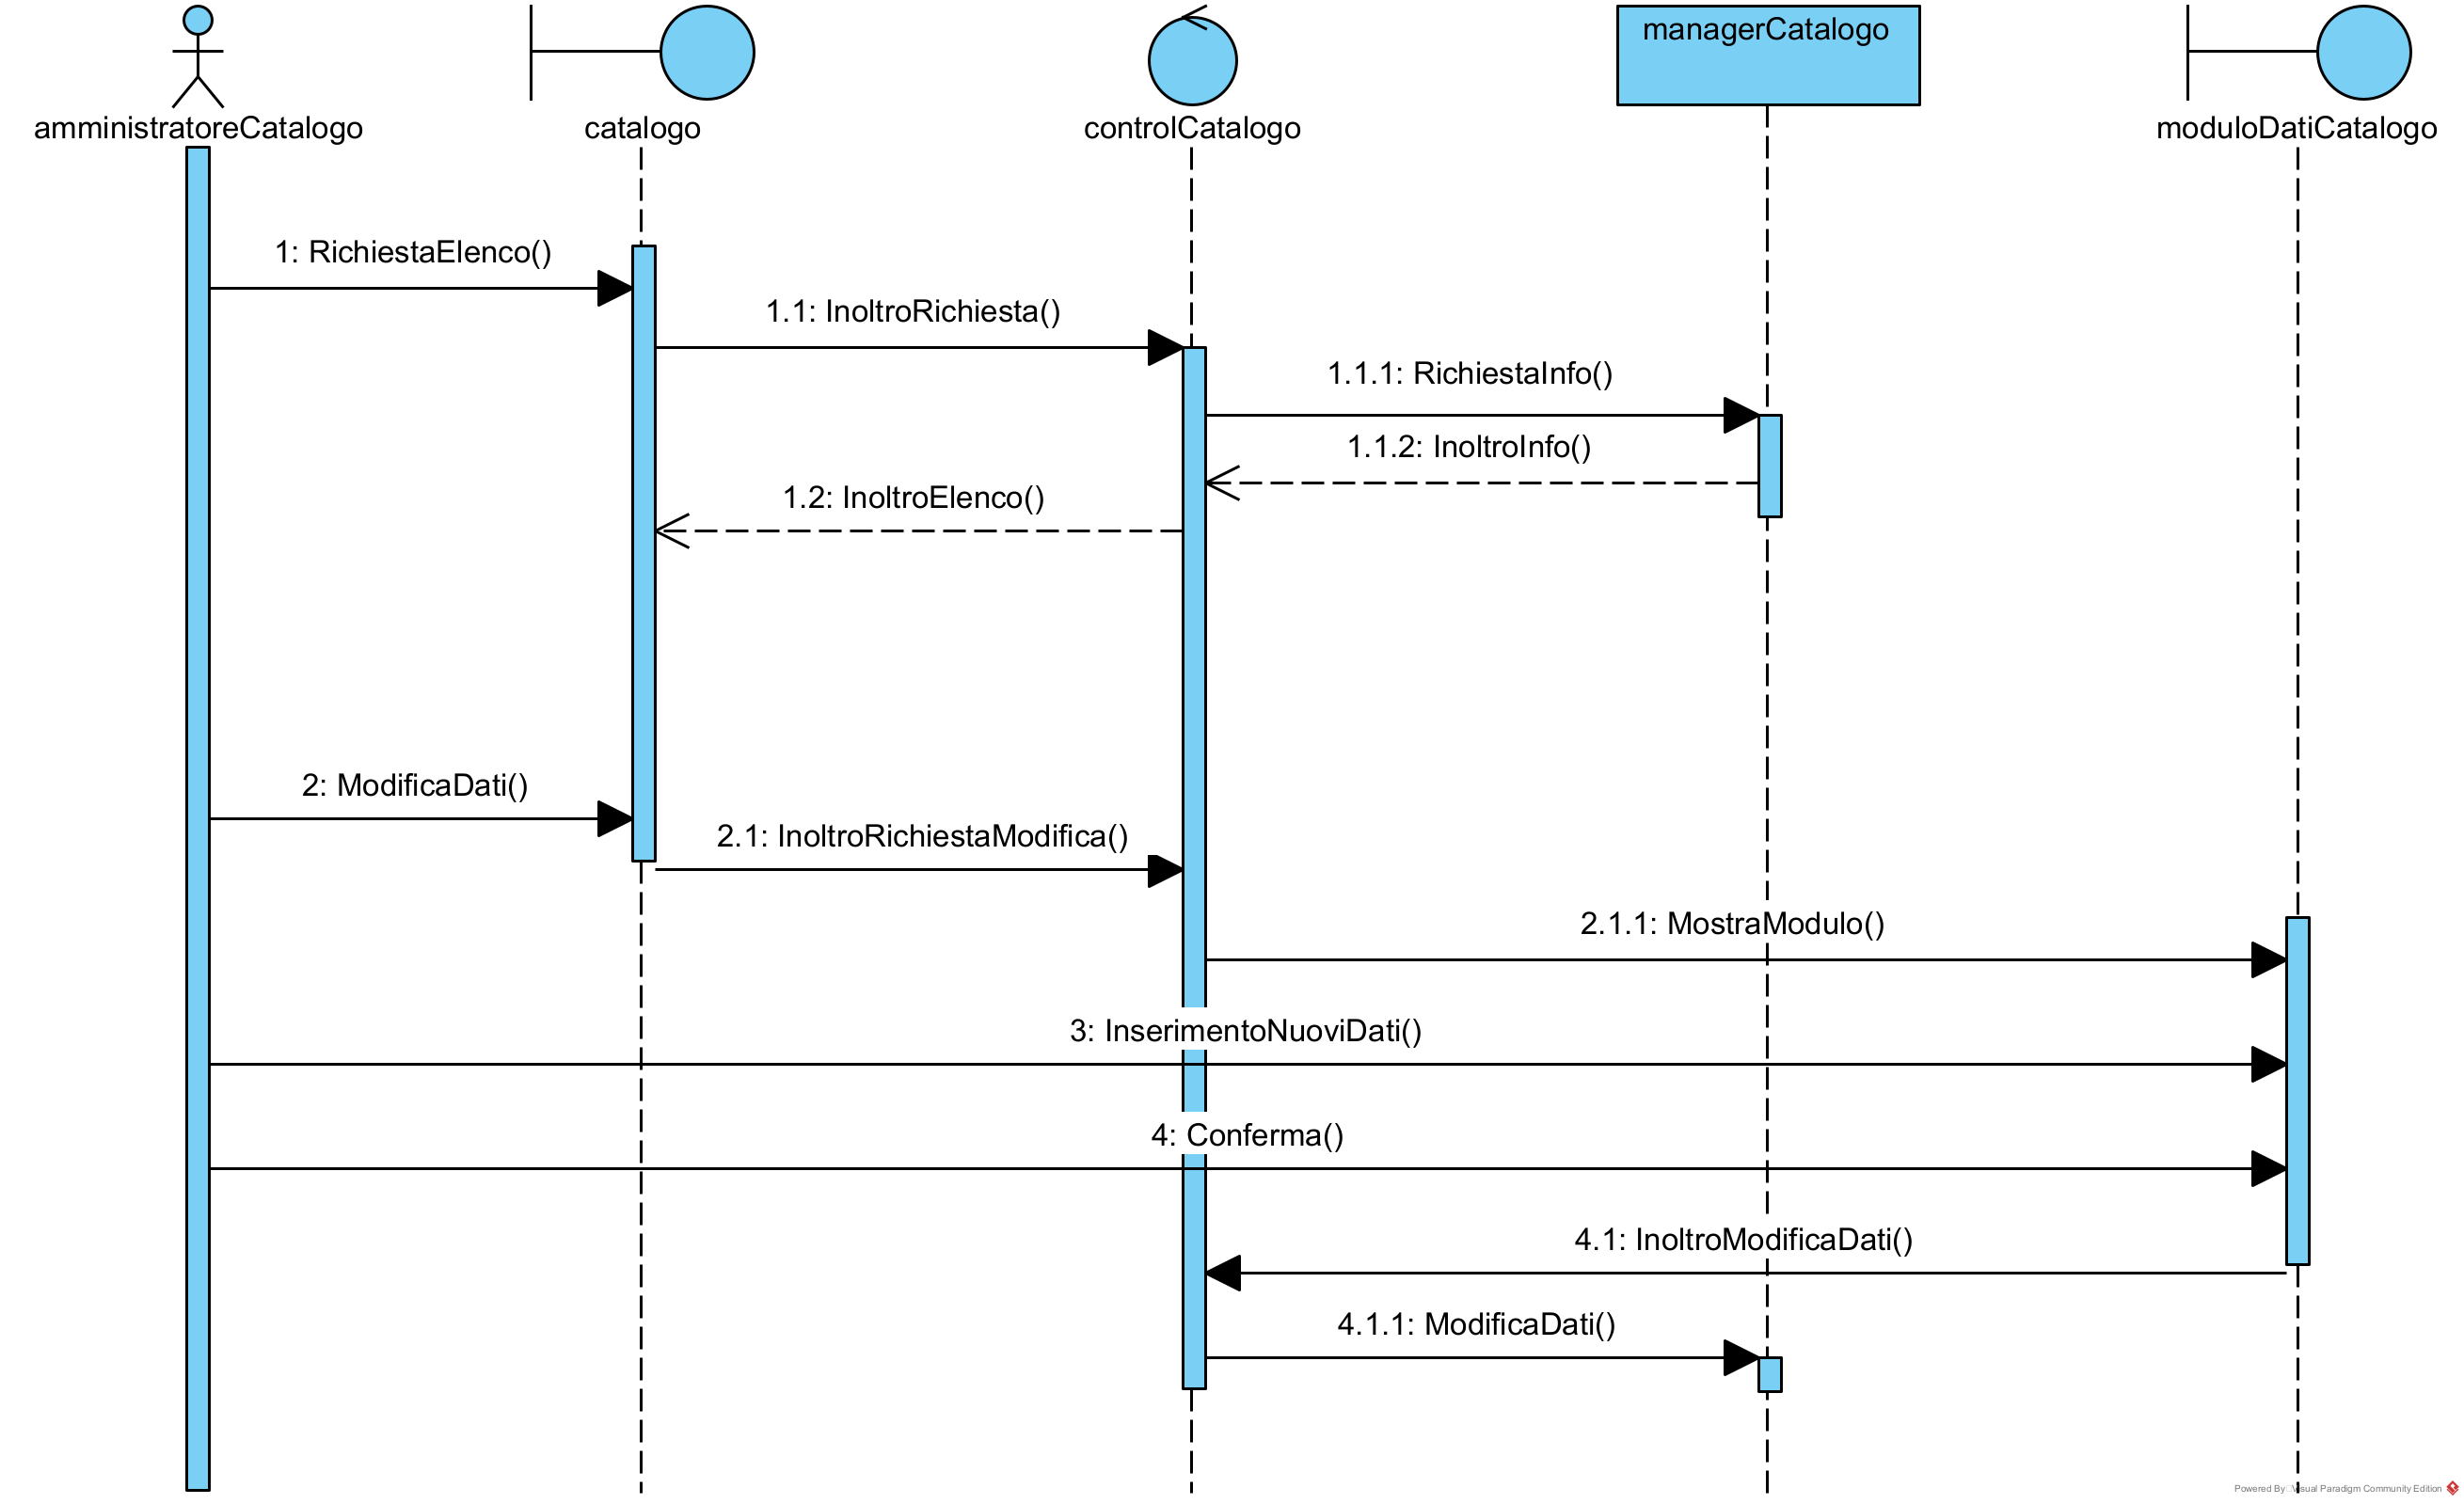
\includegraphics[height=250px]{SequenceDiagram/GestioneCatalogo}

\begin{enumerate}
\item Dall'elenco degli articoli, un amministratore fa click su quello di cui vuole modificare i dati.
\item Attraverso il controlCatalogo, l'amministratore viene reindirizzato ad un modulo in cui modificare i dati.
\item Una volta confermati i dati, il controlCatalogo inoltra la richiesta di modifica al managerCatalogo, che salva le nuove informazioni nel database.
\end{enumerate}

\section{Statechart Diagram}

\section{Activity Diagram}

\section{Navigational Path}

\section{Mock up}

\end{document}
